% !Mode:: "TeX:UTF-8"
%%%%%%%%%%%%%%%%%%%%%%%%%%%%%%%%%%%%%%%%%%%%%%%%%%%%%%%%%%%%%%%%%%%%%%%%%%%%%%%%
%          ,
%      /\^/`\
%     | \/   |                CONGRATULATIONS!
%     | |    |             SPRING IS IN THE AIR!
%     \ \    /                                                _ _
%      '\\//'                                               _{ ' }_
%        ||                     hithesis v3                { `.!.` }
%        ||                                                ',_/Y\_,'
%        ||  ,                   dustincys                   {_,_}
%    |\  ||  |\          Email: yanshuoc@gmail.com             |
%    | | ||  | |            https://yanshuo.site             (\|  /)
%    | | || / /                                               \| //
%    \ \||/ /       https://github.com/dustincys/hithesis      |//
%      `\\//`   \\   \./    \\ /     //    \\./   \\   //   \\ |/ /
%     ^^^^^^^^^^^^^^^^^^^^^^^^^^^^^^^^^^^^^^^^^^^^^^^^^^^^^^^^^^^^^^
%%%%%%%%%%%%%%%%%%%%%%%%%%%%%%%%%%%%%%%%%%%%%%%%%%%%%%%%%%%%%%%%%%%%%%%%%%%%%%%%
\documentclass[fontset=mac,type=master,campus=harbin]{hithesisbook}
% 此处选项中不要有空格
%%%%%%%%%%%%%%%%%%%%%%%%%%%%%%%%%%%%%%%%%%%%%%%%%%%%%%%%%%%%%%%%%%%%%%%%%%%%%%%%
% 必填选项
% type=doctor|master|bachelor|postdoc
%%%%%%%%%%%%%%%%%%%%%%%%%%%%%%%%%%%%%%%%%%%%%%%%%%%%%%%%%%%%%%%%%%%%%%%%%%%%%%%%
% 选填选项(选填选项的缺省值已经尽可能满足了大多数需求,除非明确知道自己有什么
% 需求)
% campus=shenzhen|weihai|harbin
%   含义:校区选项,默认harbin
% glue=true|false
%   含义:由于我工规范中要求字体行距在一个闭区间内,这个选项为true表示tex自
%   动选择,为false表示区间内一个最接近版心要求行数的要求的默认值,缺省值为
%   false。
% tocfour=true|false
%   含义:是否添加第四级目录,只对本科文科个别要求四级目录有效,缺省值为
%   false
% fontset=windows|mac|ubuntu|fandol|adobe
%   含义:设置字体,若不指定会自动识别系统,然后设置字体。fandol是开源字体,自行
%   下载安装后设置使用。windows是中易字库,窝工默认常用字体,绝对没毛病。mac和
%   ubuntu 默认分别是华文和思源字库,理论上用什么字库都行。后两种字库的安装方法
%   到谷歌上百度一下什么都有了。Linux非ubuntu发行版、非x86架构机器等如何运行可到
%   github issue上讨论。
% tocblank=true|false
%   含义:目录中第一章之前,是否加一行空白。缺省值为true。
% chapterhang=true|false
%   含义:目录的章标题是否悬挂居中,规范中要求章标题少于15字,所以这个选项
%   有无没什么用,除了特殊需求。缺省值为true。
% fulltime=true|false
%   含义:是否全日制,缺省值为true。非全日制如同等学力等,要在cover中设置类
%   型,封面中不同格式
% subtitle=true|false
%   含义:论文题目是否含有副标题,缺省值为false,如果有要在cover中设置副标
%   题内容,封面中显示。
% newgeometry=one|two|no
%   含义:规范中的自相矛盾之处,版芯是否包含页眉页脚,旧方法是按照包含页眉
%   页脚来设置。该选项是多选选项,如果设置为no,则版新为旧模板的版芯设置方法,
%   如果设置该选项one或two,分别对应两种页眉页码对应版芯线的相对位置。第一种
%   是严格按照规范要求,难看。第二种微调了页眉页码位置,好一点。默认two。
% debug=true|false
%   含义:是否显示版芯框和行号,用来调试。默认否。
% openright=true|false
%   含义:博士论文是否要求章节首页必须在奇数页,此选项不在规范要求中,按个
%   人喜好自行决定。 默认否。注意,窝工的默认情况是打印版博士论文要求右翻页
%   ,电子版要求非右翻页且无空白页。如果想DIY(或身不由己DIY)在什么地方右
%   翻页,将这个选项设置为false,然后在目标位置添加`\cleardoublepage`命令即
%   可。
% library=true|false
%   含义:是否为提交到图书馆的电子版。默认否。注意:如果设置成true,那么
%   openright选项将被强制转换为false。
% capcenterlast=true|false
%   含义:图题、表题最后一行是否居中对齐(我工规范要求居中,但不要求居中对
%   齐),此选项不在规范要求中,按个人喜好自行决定。默认否。
% subcapcenterlast=true|false
%   含义:子图图题最后一行是否居中对齐(我工规范要求居中,但不要求居中对齐
%   ),此选项不在规范要求中,按个人喜好自行决定。默认否。
% absupper=true|false
%   含义:中文目录中的英文摘要在中文目录中的大小写样式歧义,在规范中要求首
%   字母大写,在work样例中是全大写。该选项控制是否全大写。默认否。
% bsmainpagenumberline=true|false
%   含义:由于本科生论文官方模板的页码和页眉格式混乱,提供这个选项自定义设
%   置是否在正文中显示页码横线,默认显示。
% bsfrontpagenumberline=true|false
%   含义:由于本科生论文官方模板的页码和页眉格式混乱,提供这个选项自定义设
%   置是否在前文中显示页码横线,默认显示。
% bsheadrule=true|false
%   含义:由于本科生论文官方模板的页码和页眉格式混乱,提供这个选项自定义设
%   置是否显示页眉横线,默认显示。
% splitbibitem=true|false
%   含义:参考文献每一个条目内能不能断页,应广大刀客要求添加。默认否。
% newtxmath=true|false
%   含义:数学字体是否使用新罗马。默认是。
% chapterbold=true|false
%   含义:本科生章标题在目录和正文中是否加粗
% engtoc=true|false
%   含义:非博士生需要添加英文目录的,手动添加,如果是博士,此开关无效
% zijv=word|regu
%   含义:字距设置为规范规定33个字还是word中34个字。默认regu。
% citetwo=comma|endash
%   含义:相邻两个参考文献中的连接符是由逗号:[1,2]还是短线[1-2]。默认endash
%%%%%%%%%%%%%%%%%%%%%%%%%%%%%%%%%%%%%%%%%%%%%%%%%%%%%%%%%%%%%%%%%%%%%%%%%%%%%%%%
\usepackage{hithesis}

\usepackage{tcolorbox} % 颜色box
\newtcolorbox{promptbox}[1]{colback=cyan!5!white,colframe=cyan!75!black,title=#1}

\graphicspath{{figures/}}

\begin{document}
\frontmatter
% !Mode:: "TeX:UTF-8"

\hitsetup{
  %******************************
  % 注意:
  %   1. 配置里面不要出现空行
  %   2. 不需要的配置信息可以删除
  %******************************
  %
  %=====
  % 秘级
  %=====
  statesecrets={公开},
  natclassifiedindex={TP311},
  intclassifiedindex={004.02},
  %
  %=========
  % 中文信息
  %=========
  % ctitleone={局部多孔质气体静压},%本科生封面使用
  % ctitletwo={轴承关键技术的研究},%本科生封面使用
  ctitlecover={面向质量评估的代码变更影响分析及其可视化研究},%放在封面中使用,自由断行
  ctitle={面向质量评估的代码变更影响分析及其可视化研究},%放在原创性声明中使用
  % csubtitle={一条副标题}, %一般情况没有,可以注释掉
  cxueke={工学},
  csubject={软件工程},
  caffil={计算学部},
  cauthor={李美娜},
  csupervisor={苏小红教授},
  % cassosupervisor={蒋远}, % 副指导老师
  % ccosupervisor={某某某教授}, % 联合指导老师
  % 如果是深圳本科毕业论文,需要取消注释下一行,并将内容改为“规范”中要求的封面第一页最下方的日期
  szshortcdate={2022年6月},
  % 日期自动使用当前时间,若需指定按如下方式修改:
  %cdate={超新星纪元},
  cstudentid={9527},
  cstudenttype={学术学位论文}, %非全日制教育申请学位者
  cnumber={no9527}, %编号
  cpositionname={哈铁西站}, %博士后站名称
  cfinishdate={20XX年X月---20XX年X月}, %到站日期
  csubmitdate={20XX年X月}, %出站日期
  cstartdate={3050年9月10日}, %到站日期
  cenddate={3090年10月10日}, %出站日期
  %(同等学力人员)、(工程硕士)、(工商管理硕士)、
  %(高级管理人员工商管理硕士)、(公共管理硕士)、(中职教师)、(高校教师)等
  %
  %
  %=========
  % 英文信息
  %=========
  etitle={Code Impact Change Analysis and Visualization for Quality Evaluation},
  % esubtitle={This is the sub title},
  exueke={Engineering},
  esubject={Software Engineering},
  eaffil={\emultiline[t]{Faculty of Computer}},
  eauthor={Li Meina},
  esupervisor={Prof. Su Xiaohong},
  % eassosupervisor={XXX},
  % 日期自动生成,若需指定按如下方式修改:
  edate={December, 2017},
  estudenttype={Master of Art},
  %
  % 关键词用“英文逗号”分割
  ckeywords={代码审查, 代码质量评估, 变更影响分析, 代码度量},
  ekeywords={code review, code quality assessment, change impact analysis, Code Metrics},
}

\begin{cabstract}

  随着软件系统规模和复杂性不断增加,传统依赖经验丰富的专家进行人工代码审查的方法,已难以满足日益复杂的需求。由于代码审查的主要目的是确保代码质量符合项目要求,因此,自动化代码质量评估方法的重要性愈加凸显。特别是在大型软件系统中,随着开发团队的不断扩大和系统复杂度的提升,代码结构往往在漫长的维护过程中逐渐退化,模块化设计逐步被复杂的代码结构所取代,导致系统的维护和管理变得愈加困难。在软件系统的维护过程中,代码变更几乎是不可避免的,而这些变更可能对现有代码的质量和系统整体结构产生深远的负面影响,从而加剧系统的维护难度。

  本文面向代码质量评估,深入研究代码变更影响分析方法,并结合质量评估度量,通过代码审查图的方式展示C/C++项目的质量评估结果,方便开发人员从宏观的角度理解软件架构和代码质量。

  首先,本文基于代码中间表示对软件质量度量指标进行计算,基于clang提取软件项目代码的抽象语法树,进一步从抽象语法树中提取方法摘要表和全局变量信息表。这些代码中间表示蕴含了代码调用等互相依赖的特征,基于这些中间表示,本文从内聚度、耦合性、代码复杂度和代码缺陷四个角度,提取了相关的代码质量评估度量和信息。这些度量不仅帮助开发人员深入洞察了代码质量,也为后续的代码优化和维护决策提供了优化角度。

  其次,本文进一步研究了代码变更影响分析方法,以帮助开发人员更好地了解软件项目在维护过程中可能出现的相互影响的情况。变更影响分析方法能够预测代码变更可能带来的影响,帮助开发人员做出更加合理的设计和优化决策,减少变更带来的风险。本文首先实现了基于传统依赖关系闭包的变更影响分析方法,随后提出了三种新的变更影响分析方法,分别基于代码克隆、数据挖掘和深度学习技术。实验结果表明,这三种新方法均在不同的角度优于传统的依赖关系闭包方法,并能够弥补传统方法的不足之处。

  最后,为了便于开发人员和审查人员从宏观角度全面了解软件项目的架构和代码质量,本文将代码质量分析结果通过代码审查图的形式展示给用户,此外,还生成了详细的代码质量检测报告。研究表明,代码审查图能够帮助开发人员快速聚焦于特定开发模块,使其在不需要掌握过多代码上下文的情况下,便能了解代码的整体架构。同时,代码质量检测报告以清单形式展示了项目中各项质量度量,为开发人员提供了清晰的项目质量状况概览。
\end{cabstract}

\begin{eabstract}
  As the scale and complexity of software systems continue to increase, the traditional method of relying on experienced experts for manual code reviews has become inadequate to handle the increasingly complex code review demands. As a result, the importance of automated code quality assessment methods has become more prominent. In large software systems, as development teams expand and system complexity increases, the code structure often deteriorates over time during maintenance, with modular design being gradually replaced by complex code structures. This leads to greater difficulty in maintaining and managing the system. Furthermore, code changes are almost inevitable during the maintenance of software systems, and these changes can have a profound impact on the quality of the existing code and the overall system structure, thus exacerbating the difficulty of system maintenance.

  This paper focuses on code quality assessment, conducting in-depth research on change impact analysis methods, and combines quality assessment metrics to present the quality evaluation results of C/C++ projects in the form of code review graphs. This approach allows developers to better understand the software architecture and code quality from a macro perspective.
  
  First, this paper calculates software quality metrics based on intermediate code representations, extracting the abstract syntax tree of software projects using Clang, and further extracting method summary tables and global variable information tables from the abstract syntax tree. These intermediate code representations capture dependencies such as code calls, and based on these representations, this paper extracts relevant code quality metrics and information from the perspectives of cohesion, coupling, code complexity, and code defects. These metrics provide developers with deep insights into code quality and offer optimization directions for subsequent code optimization and maintenance decisions.
  
  Second, this paper further explores change impact analysis methods to help developers better understand the potential interdependencies that may arise during the maintenance of software projects. Change impact analysis methods can predict the possible effects of code changes, helping developers make more reasonable design and optimization decisions, thereby reducing the risks brought by changes. The paper first implements the traditional change impact analysis method based on dependency closure, and then proposes three new change impact analysis methods based on code cloning, data mining, and deep learning techniques. Experimental results show that these three new methods outperform the traditional dependency closure approach and effectively address its shortcomings.
  
  Finally, to help developers and reviewers gain a comprehensive understanding of the software project's architecture from a macro perspective, this paper presents the results of code quality analysis in the form of code review graphs. Additionally, detailed code quality inspection reports are generated. The study shows that code review graphs can help developers quickly focus on specific development modules, enabling them to understand the overall code architecture without needing to grasp excessive code context. Meanwhile, the code quality inspection report presents project quality indicators in a checklist format, providing developers with a clear overview of the project's quality status.
\end{eabstract}
 % 封面
\makecover
% \begin{denotation}
\begin{table}[h]%此处最好是h
\caption{国际单位制中具有专门名称的导出单位}
\vspace{0.5em}\centering\wuhao
\begin{tabular}{ccccc}
\toprule
量的名称&单位名称&单位符号&其它表示实例\\
\midrule
频率&赫[兹]&Hz&s-1\\
\bottomrule
\end{tabular}
\end{table}
\end{denotation}
%物理量名称表,符合规范为主,有要求添加
\tableofcontents %目录
\mainmatter
% !Mode:: "TeX:UTF-8"

\chapter{绪论}

\section{课题研究的背景和意义}

在软件的生命周期中,持续的代码维护是保证系统长期稳定发展的关键环节。研究表明,软件系统的维护成本在长期的项目预算中占据了60\%至80\%的比例\cite{2012Maintenance}。维护过程中,开发人员不仅要对现有代码进行修改,还要确保新增功能或修复的缺陷不会影响系统原有的稳定性和性能。为了确保软件质量,维护工作通常依赖于系统的回归测试和代码审查。具体来说,标准的代码开发流程通常包括以下三个主要步骤,如图1-1所示。

\begin{figure}[h]
\centering
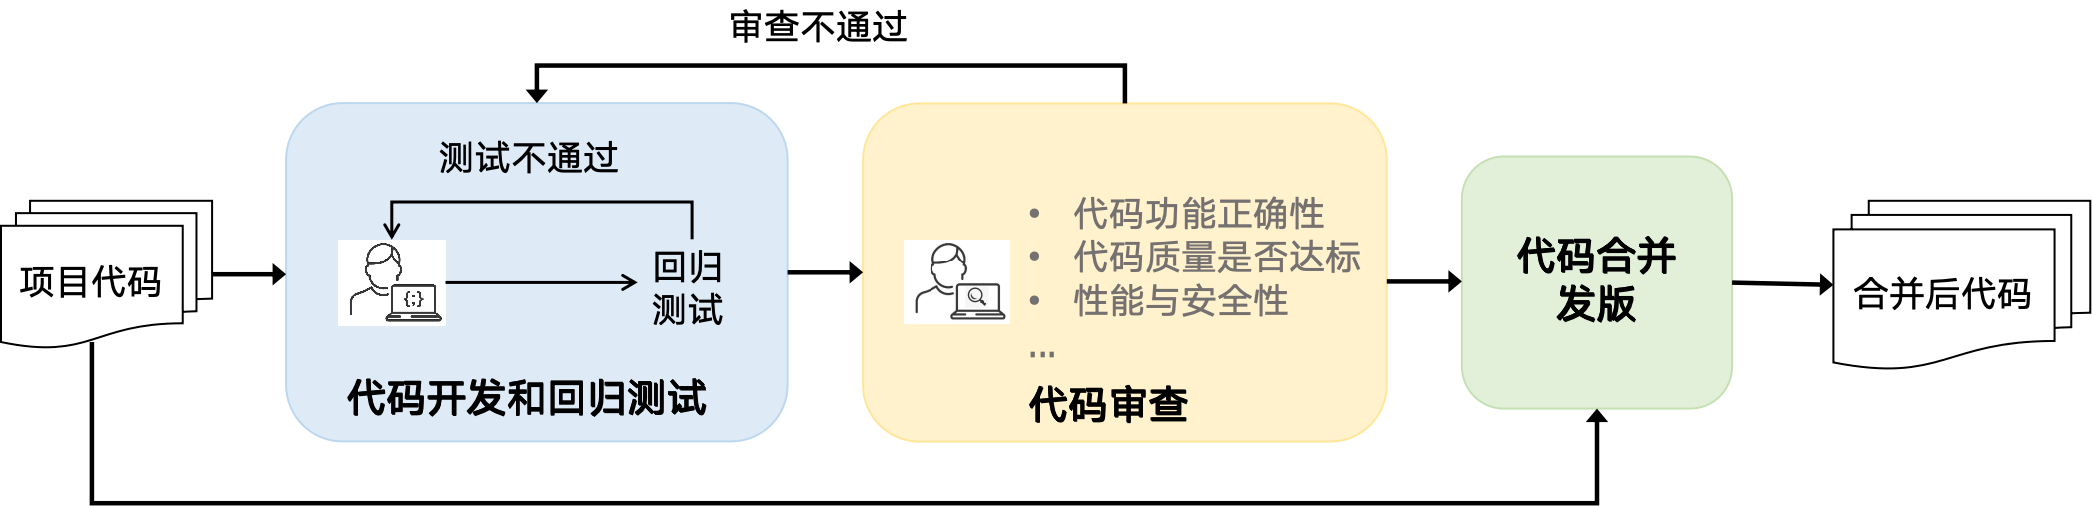
\includegraphics[width = 1.0\textwidth]{代码开发流程.png}
\caption{标准代码开发流程}
\end{figure}

(1)代码开发与回归测试:开发人员在对项目代码进行修改后,首先对修改部分进行回归测试,验证新功能是否符合需求并避免新缺陷的引入。

(2)代码审查:当测试通过后,代码将提交给审查人员进行审查。代码审查不仅仅是对代码逻辑正确性的检查,更是一个确保代码质量的重要环节。通过代码审查可以识别潜在的错误,提出代码优化建议,并统一开发团队的编码风格,从而提高代码的可维护性和可靠性。

(3)代码合并:审查通过后,修改的代码可以与原始项目进行合并,进入下一个开发周期。在此过程中,确保代码的正确性和稳定性是至关重要的,避免因合并而引入新的问题。

不论在哪一个环节,代码质量都是最重要的主题之一。而代码质量评估则是确保软件项目高效、可维护和可扩展的基础手段。随着软件系统的规模和复杂性的不断增长,代码质量直接影响到系统的稳定性、可维护性以及开发过程中的效率。尤其对于遗留系统等大型系统来讲,复杂庞大的结构和长期维护导致的系统架构腐化会让开发者在进行软件维护的时候非常困扰,常常有“牵一发而动全身”的效应,担心代码变更对系统功能的潜在不良影响。

变更影响分析(Change Impact Analysis,CIA)作为一种有效方法,能够在代码变更发生时预测变更可能带来的影响,帮助开发人员更好地理解变更对其他模块或代码的潜在影响,从而做出更加合理的设计和优化决策。因此,从代码变更影响分析的角度出发,不仅能深入理解代码变更对系统整体和各个子模块的潜在影响,还能够提高维护项目的效率\cite{2022An}。而现有的变更影响分析方法通常只关注基于静态依赖关系的影响,然而软件系统中最难以被用户察觉到,也是最容易导致功能上变更问题的是逻辑上的变更影响关系,正是因为这一类影响关系,才导致大型系统的变更如此棘手,因此如何挖掘这类关系,分析这类关系导致的质量问题成为亟待解决的难题。

在大型软件系统中,开发者在阅读代码、掌握系统架构及模块间的关系时,常常缺乏一种与代码结构深度结合的直观展示方式。通常,开发者只能依赖于肉眼阅读代码或通过开发工具生成的类图等工具进行分析,然而这些方法所提供的信息往往是碎片化的,难以呈现系统整体的架构和模块间的依赖关系。此外,在进行代码变更时,开发者也面临着难以全面、准确地评估变更影响范围的问题,尤其是在大型系统中,单一变更可能对多个模块产生深远影响。现有的分析工具虽然能揭示代码结构或潜在问题,但难以提供系统化的、直观的质量评估。

本文从代码变更影响分析入手,提出了基于代码预训练模型和基于检索增强生成的变更影响分析方法,弥补传统方法只关注依赖型影响的不足,帮助开发者更全面、安全地进行代码维护工作。同时提出了代码审查图的软件结构和质量信息可视化方式,将分析结果结合软件代码架构直观地展示给用户,帮助开发者和审查人员更直观地理解整个项目的质量情况和代码结构,优化项目的持续维护过程,提高代码维护过程的安全性和效率。


\section{国内外研究现状及分析}

变更影响分析(Change Impact Analysis,CIA)是软件工程中用于分析代码变更对系统其他部分可能产生的影响的一种技术。研究表明,代码变更对代码质量的影响在大规模软件中尤为显著。Wenchen 等人的研究指出\cite{2013Large},在大型系统中,每个版本的补丁可能影响约 2\% 的代码,这对全面的程序回归测试提出了巨大挑战。因此,针对受变更影响的代码区域进行精确测试则是一种既高效又安全的测试方案。此方法不仅能够有效降低时间和资源成本,还能在不牺牲系统质量的前提下,减少因回归测试覆盖不足而引发的潜在漏洞或故障风险。这一策略强调了将代码变更范围与回归测试策略精细化结合的重要性,为提升软件开发和维护阶段的代码质量提供了有力支持。

自Arnold等人\cite{Arnold1996}提出变更影响分析的概念以来,它一直是代码审查的重要组成部分之一。该方法支持用户在代码变更之前对其影响进行分析,从而估计变更可能造成的负面影响,其优势可总结如下:(1)能提升代码的稳定性和可靠性\cite{KRETSOU2021110892}。通过分析代码变更对相关模块的影响,开发者可以识别潜在的故障或不一致之处,在变更合入前发现问题,避免引入新的缺陷,从而提高系统的稳定性和可靠性。(2)有助于模块化设计和低耦合。变更影响分析能够反映出代码模块之间的依赖关系和耦合程度,通过减少不必要的耦合,增强代码的模块化特性,从而提升代码的可维护性和可扩展性。(3)有助于代码质量的提高。通过变更影响分析能够记录变更过程中的风险评估和解决措施,满足质量保证和审查的需求,提高软件开发过程的透明性和可追踪性。(4)有助于开发团队协作。变更影响分析为团队提供了清晰的变更范围和影响信息,便于团队成员之间协调工作,减少因沟通不足导致的重复工作或冲突,同时提高代码可读性,有助于开发团队更快速地理解系统,减少后期维护成本。

变更影响分析方法主要可分为两部分,分别是静态变更影响分析方法和动态变更影响分析方法,其中静态分析方法中还有一类特殊地关注软件代码变更历史的方法。本文主要从这两方面展开对变更影响分析方法的总结。


\subsection{静态变更影响分析方法}

静态分析方法因其具有高覆盖率和高安全性的优势,广泛应用于对安全性要求较高的软件回归测试中。这类方法主要通过传统的程序分析技术获取代码的语法和语义信息,如基于程序的中间表示(如控制流图、调用图等)来进行分析。在静态分析方法中,根据分析粒度的不同可分为过程内和过程间,分别表示分析方法内和方法间的变更影响。过程内分析方法通常依赖于程序切片、控制流和数据流等技术\cite{2004Efficient,1991Using}分析语句级别的变更影响关系,而过程间的影响分析则主要通过调用图或系统依赖图进行分析,揭示不同方法之间的依赖关系\cite{JitenderKumarChhabra2018Improved, 2011An, 2013Analyzing}。

Schrettner等人\cite{Department2013Impact}提出了一种创新的静态执行后关系(Static Execute After, SEA)方法,这是一种计算高效且足够精确的程序关系,表示代码之间的运行顺序紧密相连的情况,可以作为变更影响分析的基础。SEA的提出为程序分析提供了新的视角,其实验结果表明,通过SEA计算得到的影响关系能够发现大量的实际影响关系,显著提高了静态分析的准确性和实用性。

Sun等人\cite{5676283}提出了将变更类型与影响机制相结合的变更影响分析方法。他们认为不同类型的软件变更通常会带来不同的影响机制,因此需要根据变更的具体类型来制定相应的影响分析策略。此外,他们还指出,影响关系的精确度与初始影响关系的精确度密切相关,初始影响关系越精确,基于其计算得到的最终影响关系也会更为准确。这一发现为改进影响分析技术提供了新的思路,强调了初始数据质量对最终分析结果的重要性。

Liang等人\cite{10430003}提出了一种影响集的概念,该影响集由包、类、方法、语句和变量五个层级的影响元素组合而成。通过在这五个层级上逐层搜索受影响的节点,并对这些节点进行层次化整理,最终构建出完整的层级影响结构。在此基础上,他们利用变更集定位子语句级依赖关系图中的变更节点,从多个层次分析代码变更的影响范围。

在静态分析研究中,基于图的分析方法是常见的手段之一。Ufuktepe等人\cite{2021Code}针对方法间的依赖关系,利用方法调用图和影响图,提出了一种基于马尔可夫链的变更预测方法。他们通过前向切片信息计算变更后的影响概率,实验结果表明,调用图的精确率更高,而影响图则在少数情况下有更高的召回率。Peng等人\cite{2022An}针对传统C程序影响分析工具仅能在方法粒度上进行分析的局限性,研究了一种基于语句粒度的变更影响分析方法。该方法首先对源代码文件进行编译,提取全局信息以生成控制流图和调用图等结构。随后,将变更代码解析为不同类型变量的组合,并结合程序结构和变量变更信息进行深入的影响分析,从而更精确地评估代码变更带来的影响范围。

近年来,一些研究者尝试利用深度学习模型来研究代码变更的影响分析。Zhang等人\cite{10366673}提出了一种方法,通过构建更精细的系统依赖图并使用程序切片技术定位变更代码的影响区域,将这些区域提取为变更影响图。随后,他们采用GCN(图卷积网络)从变更影响图中提取上下文信息,并将其与抽象语法树中的语法变更数据结合起来,最终实现了对不同版本维护类型的识别。Jiang等人\cite{姜瑛2024基于动态}提出了一种基于动态AST和GCN的代码变更影响范围分析方法。该方法首先对 DAST 的token信息进行了拓展,随后,提出了基于 DAST 的代码依赖分析的类型和具体的分析方法。在完成 DAST 节点权重矩阵的构建之后,运用基于 GCN 的代码变更影响范围分析模型,进而确定代码的变更影响范围。根据实验结果,该方法较为有效地分析了方法内变更影响范围。

随着软件系统复杂度的增加,单一的变更影响分析方法已经难以满足高效性和准确性的双重需求。因此,研究人员提出了混合变更影响分析技术,通过将多种CIA方法结合起来,以提高变更影响分析的准确性和健壮性\cite{2021Improving}。混合CIA技术的核心思想是将不同方法的优势互补,从而弥补单一方法的不足。研究表明,结合至少两种CIA技术的混合策略能够显著提高性能,且相比于基线技术,混合CIA方法始终表现出更好的性能改进。这一进展为变更影响分析提供了新的解决方案,尤其适用于大型复杂系统的影响分析任务。


\subsection{动态变更影响分析方法}

尽管静态影响分析在软件工程中因其较高的覆盖率和较好的安全性而被广泛应用,但其分析结果往往存在误报较高的问题。这是因为静态分析主要依赖程序的中间表示(如控制流图、调用图等)进行推理,而这些模型无法捕捉程序在运行过程中可能出现的实际行为。与静态分析不同,动态影响分析是在程序运行时收集实际执行信息,并基于这些运行时数据计算程序中各个部分的影响关系。

在面向对象编程的系统中,由于程序实体之间的依赖关系较为复杂且难以静态建模,动态分析的结果有时会产生不精确性的影响。为了提高动态分析的精确性,Huang等人\cite{2007Precise}提出了一种专门针对面向对象程序的精确动态变更影响分析方法。该方法结合了面向对象编程的特性,能够更加准确地确定程序实体之间的实际影响关系。同时,Huang等人通过排除与变更对象无关的程序部分,显著减少了分析的规模,从而提升了分析的效率和精度。

在动态变更影响分析的精确性和可靠性方面,Cai等人\cite{2015Acom,2014Estimating}进行了深入研究。他们提出了一种实验方法,首先通过敏感性分析来评估变更影响分析的准确性,然后通过实施软件变更并观察这些变更的实际影响,进一步分析其精确度和召回率。这一方法为动态影响分析技术的有效性提供了重要的实证依据,并揭示了在实际应用中可能遇到的挑战。此外,Cai等人还提出了针对分布式系统的动态影响分析方法——DISTIA\cite{2016DistIA}。该方法通过对分布式系统中各个执行事件进行部分排序,并根据这些排序推断事件之间的因果关系,同时结合消息传递的语义预测影响在不同进程边界内外的传播情况,有效地解决了分布式系统中的影响传播问题,为分布式软件的动态影响分析提供了新的技术路径。

Wang等人\cite{王海龙0一种基于代码树分析的代码影响范围分析方法}通过词法分析器和语法分析器对源代码进行处理,将其转化为令牌和解析树,并为抽象语法树的每个节点设置预定义的权重。他们结合动态分析技术,收集代码运行时数据,并研究抽象语法树与运行时信息之间的关系,得出关联分析结果。在此基础上,构建代码影响图,并对其进行深入分析,研究代码变更如何通过影响图传播,从而得出扩散分析的结论。同时,他们追踪代码变更在抽象语法树中的传播路径,评估其可能带来的影响范围。

尽管动态分析通常能够提供更为精确的结果,但其成本较高,而且在面对复杂的系统时,无法确保分析结果的完全安全性。

\subsection{其他代码变更影响分析方法}

除了上述静态和动态分析方法外,另一些研究并未直接关注软件本身,而是将关注点转向软件变更的历史库\cite{2011An, Markus2017Supporting, 2008Mining, 2014Impact, 2016Generalizing}。这些研究认为,软件变更历史记录中包含了大量与程序及其演化相关的信息,分析和挖掘这些信息能够帮助识别和预测变更对软件系统的潜在影响。这些依赖关系和变更模式可以通过数据挖掘方法、信息检索技术以及机器学习等手段进行挖掘和分析,从而为变更影响分析提供新的视角和方法。

Gethers等人\cite{2011An}采用了信息检索、动态分析和数据挖掘方法,基于历史源代码提交记录改进了变更影响方法的生成技术。通过分析过去的源代码提交,研究者能够更好地识别变更和其他程序部分之间的潜在依赖关系,从而生成更加精确的变更影响集。这一方法突出了历史数据的重要性,利用现有的变更历史信息来为未来的变更影响分析提供依据,从而提升了分析的准确性和效率。

Zanjani等人\cite{2014Impact}提出了一种结合交互历史和提交历史的方法来分析源代码变更请求。他们的创新之处在于将信息检索、机器学习和轻量级源代码分析相结合,通过构建源代码实体的语料库,来提高变更影响分析的精确度。当给定一个变更请求的文本描述时,该语料库可以被查询,并返回一个按相关性排序的最可能发生变更的源代码实体列表。这种方法能够通过历史变更请求的文本描述,准确预测哪些源代码实体可能受到影响,为开发人员提供有效的决策支持。

Rolfsnes等人\cite{2016Generalizing}致力于改进现有的耦合分析算法,尤其是在软件变更的上下文中。TARMAQ算法是他们提出的一种新型算法,在性能上明显优于传统静态分析算法。TARMAQ通过挖掘代码库中的耦合关系,能够更精确地揭示源代码之间的依赖和关联,从而提高了变更影响集的生成效率和准确性。

Huang 等人 \cite{2021Change} 使用传统变更影响方法获得变更初始影响集,将历史变更模式应用于当前的变更影响分析任务,对分析过程进行增强,有效提高了变更影响分析的准确性和效率。在实际应用中,变更影响分析通常需要处理复杂的依赖关系,通过借助历史变更模式,该方法能够提升分析过程的普适性和适应性。


\subsection{现有方法存在的问题与分析}

尽管现有的变更影响分析方法已经非常丰富,但是仍存在一些局限性。

1.对逻辑上的变更影响挖掘不够深刻

无论是静态方法还是动态方法,其本质上都是通过显式的代码间依赖关系来进行分析,即表现在代码中间表示(如调用图、影响图、抽象语法树等)中,代码元素之间的依赖关系(如图上的连通性、路径的可达性等)。然而,除了这些显式的依赖关系之外,仍然存在大量逻辑上的变更影响关系未被充分挖掘和揭示。在文献\cite{daipeng2024software}中有提到现有的变更影响分析方法忽视了因代码克隆导致的变更影响,这实际上就是逻辑型变更影响,但只是逻辑型变更影响关系的一种,项目代码仍然存在更多逻辑型的未被揭示的变更影响。正是由于其隐式影响的特点,才导致检测难度大,因此挖掘不够深刻。

而面向软件变更历史的分析方法通过挖掘开发者过往的变更行为模式来识别变更影响,在一定程度上能检测逻辑上的变更影响关系,这是由于过去的变更历史都是由开发者充分理解代码功能和语义的基础上,人工分析后变更,并且经过较为严格的审查环节才完成代码合入的过程,因此其反映的变更影响关系较为可靠和全面。但是这类方法只能利用项目内的变更历史,难以迁移到其他项目中使用。有部分研究通过分析提交信息和变更代码之间的关系来预测潜在影响,但依赖于提交信息的质量,这使得方法的准确性受到影响,尤其在提交信息质量不稳定或缺失的情况下,误差率较高。而且该类无法处理没有变更历史或缺少提交信息的项目,存在明显的局限性。


2.缺乏与代码质量和代码结构的深入结合

变更影响分析在软件代码维护过程中具有重要意义。如文献\cite{KRETSOU2021110892}所述,变更影响分析不仅能够优化软件的维护过程,还能提升代码质量与开发效率,同时帮助开发人员更深入地理解软件系统的结构和需求,从而更高效地开展开发与维护工作。然而当前研究在将检测结果与代码结构和代码质量进行深度结合这一方面仍在存在局限性。这一不足体现在多个方面。

首先,对于软件项目来说,变更影响分析通常是针对整个代码仓库展开的。但是,现有的分析结果往往呈现为一些孤立的数据和关系,没有将其与代码的实际结构紧密联系起来。开发人员在面对这些结果时,只能看到一些抽象的信息,难以清晰地了解代码的具体结构和内部关系。例如,开发者根据检测结果可得知哪些代码部分可能会受到变更的影响,但无法直观地感知这种影响是如何在代码的模块、方法等结构层次上体现的,无法明确具体的代码元素之间是如何相互关联和相互影响的。

其次,现有方法在代码质量层面的结合也不够深入。代码质量涉及可维护性、可复用性、安全性等多个维度,其中代码间的变更影响关系会直接影响到代码的可维护性,但现有研究未能与可维护性指标有机结合,除此之外,不良的隐式耦合也可能导致用户在变更时遗漏应同步变更的代码,导致代码质量的下降,甚至代码功能逻辑的不一致。缺乏直观的结果展示进一步限制了开发者对变更影响与代码质量关系的理解,难以准确把握变更对于代码质量的全面影响。


\section{本文的主要研究内容以及各章节安排}
\subsection{主要研究内容}

为解决前文变更影响分析方法存在的局限性入手,本文面向C/C++软件项目,提出基于代码预训练模型和检索增强生成的变更影响分析方法,同时提出基于代码审查图的软件结构和质量可视化方法,旨在帮助用户在软件生命周期的各个环节了解代码各个部分的变更影响关系和代码质量信息,帮助用户更安全地对软件代码进行维护。

主要研究内容分为三个部分:基于关系挖掘和预测的代码变更影响分析,基于检索增强生成的代码变更影响分析和基于代码审查图的代码结构可视化和质量评估。

(1)基于关系挖掘和预测的代码变更影响分析

这部分首先将代码转换成抽象语法树(Abstract Syntax Tree,AST)作为中间代码表示,并且基于AST提取方法定义-使用链和全局变量定义-使用链,分别整理为方法摘要表和全局变量信息表。在此基础上实现了三种变更影响分析方法。基于依赖关系方法根据方法摘要表和全局变量信息表计算依赖传递闭包得到变更影响关系。基于克隆关系的方法通过检测代码克隆反映影响关系,克隆代码指的是开发者通过复制和粘贴已有的代码片段,来创建功能类似的代码段。这种代码通常在功能上与原代码重复,因此当代码有变更的时候,这样的代码会被影响。基于共现关系的方法通过数据挖掘的方式挖掘频繁在变更历史中共同更改的代码对,反映其之间存在代码变更影响关系。将这三种方法检测得到的影响关系整合为数据集,训练代码预训练模型,对方法间变更影响关系进行预测。


(2)基于检索增强生成的代码变更影响分析

这部分针对前文方法的局限性,为了弥补基于预测方法的计算效率问题和依赖信息丢失的问题,提出基于代码依赖和检索增强生成的代码变更影响分析方法。该方法共分为三个模块,首先是数据构建模块,构建原始知识库、生成代码依赖图和嵌入模型训练所需要的三元组语料。检索模块首先训练嵌入模型,使具有变更影响关系的方法在向量空间中更近。检索时对查询方法进行编码,在知识库中检索得到候选的有变更影响关系的方法。在生成模块使用大语言模型对候选方法进行判断,得到最终的有变更影响关系的方法。

(3)基于代码审查图的代码结构可视化和质量分析

为帮助开发者全面了解软件项目的整体架构、模块化情况以及经过深入分析后的代码质量,本文提出代码审查图的概念,将整个软件项目的结构、质量度量和变更影响等信息可视化,便于开发者更直观地理解项目的各个方面,并做出相应的优化决策。在代码审查图中,节点代表项目中的关键元素,包括方法和全局变量。为了对代码质量进行量化分析,结合变更影响关系,从 5 个属性和 18 个度量元来计算代码度量,作为节点的属性。而边则表示不同节点之间的关系,包括依赖关系、耦合关系和变更影响关系。这些边反映了不同模块或方法之间的交互和依赖,能够揭示出系统架构的潜在问题和优化点。


代码审查图的可视化工作通过图可视化引擎G6完成,G6引擎能够高效地渲染和展示复杂的图结构,支持交互式查看和深入分析,帮助开发者快速识别问题所在。此外,所有提取和计算得到的质量分析结果还会以代码质量分析报告的形式进行详细总结,报告中将完整展示各项质量指标、分析结果和建议,确保开发者能够全面掌握软件项目的质量状态,从而进行有效的改进与优化。

\subsection{章节安排}

本文的章节安排如图1-2。

\begin{figure}[h]
\centering
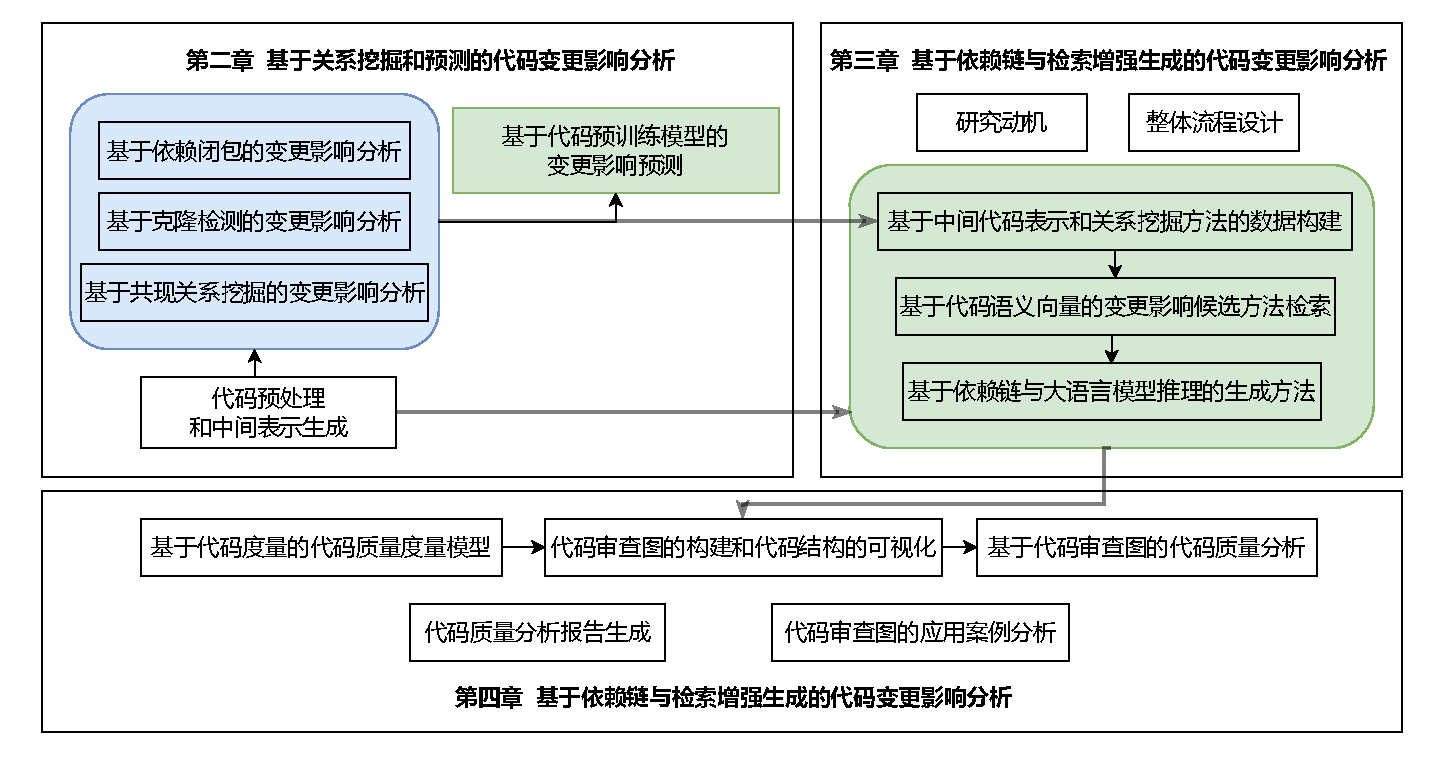
\includegraphics[width = 1.0\textwidth]{figures/1_章节结构图.pdf}
\caption{章节安排}
\end{figure}

第一章为绪论,首先介绍了本文的研究背景和研究现状,分别从静态方法、动态方法和基于代码库的方法三类分析方法总结了变更影响分析现状,进一步分析了这些方法的问题和难点。最后对论文的整体架构进行了介绍。


第二章实现了传统的基于关系挖掘的三种方法,在分析传统方法的局限性的基础上,提出了基于代码预训练模型的变更影响分析方法,最后进行了实验结果和对比分析。

第三章在第二章的基础上,提出了基于依赖链和检索增强生成的变更影响分析方法,进一步提高检测的准确率和计算效率,最后通过实验验证了方法的有效性。

第四章提出了代码审查图的概念,将变更影响关系作为节点和边的一部分,通过图可视化引擎G6对图进行可视化,并根据可视化的结果进一步对不良的代码质量模式进行总结,最后进行了实验结果展示和分析。




% !Mode:: "TeX:UTF-8"

\chapter{基于关系挖掘和预测的代码变更影响分析}

%%%%%%%%%%%%%%%%%%%%%%%%%%%%%%%%%%%%%%%%%%%%%%%%%%%%%%%%%%%%%%%%%%%%%%%%%%%%%%%
\section{引言}

软件变更是软件维护的核心环节。对软件系统的修改可能引发系统其他部分的不良副作用或连锁反应。而变更影响分析的目标在于识别变更的涟漪效应,帮助开发者安全地进行变更。方法之间的变更影响可以分为以下两种类型:

(1)依赖型变更影响关系:依赖型指的是能直接体现在代码静态结构中的变更影响关系,如将项目代码组织为抽象语法树、系统依赖图或影响图,通过图结构的可达性分析,得到的静态依赖关系。方法间的依赖型变更影响关系表现为方法间的调用或间接调用关系。

(2)逻辑型变更影响关系:在这种类型的变更影响关系中,方法之间不存在静态结构之间的关联关系,但它们的实现逻辑或所操作的数据之间存在某种隐含的关联。具体来说,这种关系可能源于它们共同维护某个数据的一致性、共享某些资源,或其功能逻辑有某种预期联系。因此,当某个方法发生变化时,可能会间接影响到其他方法的行为或结果。

依赖型影响关系可在代码的静态结构中直接显现,通过基于依赖关系的传统影响分析方法甚至开发工具即可捕捉,而逻辑型影响关系通常只能通过开发者通过阅读代码进行人工分析,这无疑增加了分析的难度。正是由于逻辑型影响的存在,开发者在维护软件代码时面临着诸多困扰,会出现难以理解软件架构、难以安全进行代码变更等问题。

为了解决上述问题,本文以C/C++项目为研究对象,针对不同的应用场景,实现了基于依赖闭包、基于克隆检测以及基于共现关系挖掘的的变更影响分析方法,在研究这三种方法各自的优点和局限性的基础上,提出了基于代码预训练模型的变更影响预测方法,并通过实验验证了基于代码预训练模型的方法的有效性。


\section{代码预处理和中间表示生成}

\subsection{基于clang的抽象语法树生成}
抽象语法树(Abstracted Syntax Tree,AST)把代码的语法结构以树形的方式进行了抽象化描述。在这个树形结构中,每一个节点都对应着代码中的某个元素,比如变量声明、语句或者是表达式等。从抽象语法树的根节点出发,代码逐步被拆解成更小的部分,直到最终到达叶节点,这些叶节点代表了代码中最基本的元素,如操作符或变量等。AST 能够清晰地展示出代码的层次和结构,为编译器或其他工具分析和处理代码提供便利。


Clang 是由苹果公司发起的支持 C、C++、Objective-C 和 Objective-C++语言的编译器前端,负责对代码进行词法分析、语法分析和语义分析,对程序代码的分析和理解至关重要\cite{clang}。而libclang 是 Clang 编译器的一个重要组成部分,它提供了一套用于解析源代码的程序接口。这些程序接口允许开发者在项目中使用 Clang 的强大语言解析和代码分析功能\cite{libclang}。本文使用libclang 生成AST ,提取代码中的调用和依赖关系,为后续进一步分析提供基础。

在 libclang 解析得到的抽象语法树中,游标(cursor)是一个核心概念,它作为一个指针或引用存在,每个 cursor 都与 AST 中的一个特定节点相对应,表示了源代码中的一个结构元素。通过操作 cursor,可以遍历整个 AST,访问和分析代码中的各种元素,如获取变量的类型、方法的参数列表、类的成员等。libclang 提供了一系列 API 函数来操作 cursor,例如:遍历 AST 中的 cursor、获取 cursor 的类型(如是否为方法定义、变量定义、变量引用等)、获取 cursor 所代表的源代码元素的名称、类型、位置等信息、获取 cursor 的父节点或子节点等。

\begin{table}[htbp]
\caption{重要AST节点类型标识}
\label{1_重要AST节点类型标识}
\vspace{0.5em}\centering\wuhao
\begin{tabular}{cc}
\toprule
节点标识 & 含义  \\
\midrule
Translation\_Unit & 一个翻译单元 \\
Function\_Decl  & 方法定义 \\
Parm\_Decl & 方法的参数定义 \\
Var\_Decl & 变量定义 \\ 
Devl\_Ref\_Expr  & 变量引用  \\
Call\_Expr  & 方法调用  \\
\bottomrule
\end{tabular}
\end{table}   

本文通过操作游标,遍历 AST,获取整个 AST的结构,并将clang定义的部分重要节点类型列在表\ref{1_重要AST节点类型标识}中。值得注意的是,在 clang 中是不区分方法声明和方法定义的,统一用 Function\_Decl来标识,区分二者主要看是否有方法体,在 libclang 中提供了程序接口供开发者调用以进行区分。

\subsection{方法调用链提取与分析}
在使用 libclang 提取代码的抽象语法树后,遍历整棵树来提取方法之间的调用关系。为了进行方法调用链分析,本文重点关注抽象语法树上的方法节点,以及方法节点内部的调用节点,分别对应着代码中方法的定义和方法内部对其他方法的调用。


\begin{algorithm}[htbp]
    \caption{方法调用链提取}
    \label{1_方法调用链提取}
    \KwIn{项目中的所有代码文件: $files$}
    \KwOut{方法摘要表: $functions$}
    \SetKwFunction{FMain}{scanAndAnalyze}  % 定义函数名字
    \SetKwFunction{FTraverse}{traverse}  % 定义函数名字
    \SetKwProg{Fn}{Function}{:}{}  % 定义函数结构
    \Fn{\FMain{$files$}}{
        $functions \gets \{\}$  $\#$ 初始化方法摘要 \;
        $\#$ 第一次扫描:收集方法的定义 \;
        \ForEach{$file \in files$}{
            $cursor \gets \text{libclang.parse}(file).cursor$ $\#$ 获取AST的根cursor \;
            \texttt{traverse(cursor, 0, functions, file, True)} $\#$ 遍历AST,收集方法定义 \;
        }
        $\#$ 第二次扫描:分析方法调用情况 \;
        \ForEach{$file \in files$}{
            $cursor \gets \text{libclang.parse}(file).cursor$ $\#$ 获取AST的根cursor \;
            \texttt{traverse(cursor, 0, functions, file, False)} $\#$ 分析方法调用 \;
        }
        \textbf{return} $functions$ \;
    }
    \Fn{\FTraverse{$node, depth, functions, filePath, isFirstScan$}}{
        \If{$isFirstScan$}{
            \If{$node.kind == CursorKind.FUNCTION\_DECL$}{
                $function \gets \text{collectionInfo}(node)$ $\#$ C收集方法信息 \;
                $functions.\text{add}(function)$ $\#$ 将方法添加到方法摘要 \;
            }
        }
        \ElseIf{$node.kind == CursorKind.CALL\_EXPR$}{
            \texttt{parse(node)} $\#$ 分析被调用的方法 \;
        }
        \ForEach{$n \in node.get\_children()$}{
            \texttt{traverse(n, depth + 1, functions, filePath, isFirstScan)} $\#$ 递归遍历子节点 \;
        }
    }
\end{algorithm}


为了对方法调用链进行分析,首先需要研究方法调用链的提取算法,具体的提取流程如算法\ref{1_方法调用链提取}所示。对抽象语法树的遍历主要分为两次,第一次遍历的目的是获取所有的方法定义。首先提取所有的Function\_Decl 节点,它表示方法的定义,在该节点中可提取方法签名。在Function\_Decl 节点下,提取子节点 Parm\_Decl,该节点表示方法的参数列表,在该节点中可提取参数名称和参数类型等参数相关信息。然后提取Function\_Decl节点的子节点 VarDecl,该节点表示在该方法内定义的局部变量。在对方法进行分析时,我们本身不关心方法的内部实现,但是由于在 C/C++语言中,存在局部变量可以和全局变量重名的情况,在这里提取方法内定义的局部变量,方便后续在提取全局变量的使用时,排出同名局部变量的影响。除此之外,还需提取整个方法的 token 序列,所在文件以及作用域。


第二次遍历的目的是提取方法之间的调用关系。提取 Function\_Decl 节点
的子节点 Call\_Expr,该节点标签表示的是调用语句,可提取调用的方法名。注意,由于主要分析该项目中由开发者定义的方法之间的依赖关系,所以对于一些标准库方法的调用选择忽略,不进行提取。

分析结束后,将会获得每个方法的方法调用关系和详细信息,将提取到的信息组织为一个方法摘要表,表的每一项表示一个方法的摘要,每个摘要由\textless \textit{funcID}, \textit{token}, \textit{params}, \textit{call}, \textit{scope}, \textit{file}, \textit{localvar} \textgreater 共7部分组成,分别表示方法的唯一ID标识,方法体,方法参数列表。方法内调用的其他方法,方法的作用域,方法所在模块和方法定义的局部变量。


\subsection{全局变量定义-使用链提取与分析}
在C/C++代码中,相同描述符修饰下的全局变量的定义、作用域、生命周期和方法是同级别的,所以在本文中,将全局变量也作为独立的代码单元进行分析。
全局变量定义-引用链的提取和方法的定义和调用提取类似,对 AST 的遍历主
要也分为两次。
% 具体流程如图\ref{1_全局变量提取流程图}。

% \begin{figure}[h]
% \centering
% 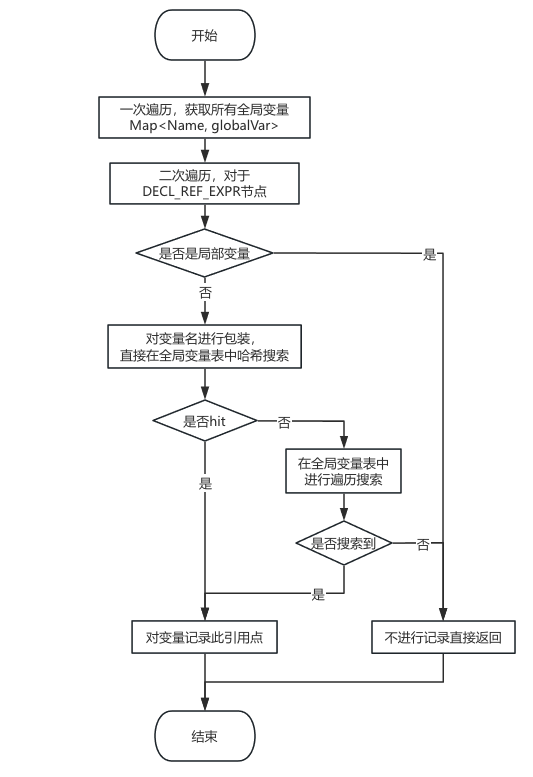
\includegraphics[width = 0.7\textwidth]{全局变量提取流程图.jpg}
% \caption{全局变量提取流程图}
% \label{1_全局变量提取流程图}
% \end{figure}

第一次遍历获取所有的全局定义。首先提取所有的
Var\_Decl 节点,它表示变量定义,然后提取节点中的变量名和变量类型。注
意,由于在 AST 中的节点标签中无法区分变量是否是全局的,所以这里根据节点在 AST
中的深度来判断是否是全局变量,并且在变量名前加上针对该项目文件的绝对路径,来
保证变量名的唯一性。在确定其为全局变量后,还需进一步提取该变量的作用域。在
C/C++语言中,static关键字可用于修饰变量和方法,意味着该变量或该方法只能在其所在文
件内使用,而不是全局可用,因此需要对其作用域进行判断。一次遍历提取到的结果是
一个全局变量表,这里使用哈希表 Map<Name, globalVar>的数据结构进行存储,方便对
全局变量进行查找。

第二次遍历的主要目的是提取全局变量的引用点。在方法节点子树中搜索
Devl\_Ref\_Expr 节点,该类型节点表示对变量的引用,这里首先判断被引用的变量是否是局部
变量,根据方法摘要表中该方法的相关信息可以判断,如果是则直接返回,因为我们不关心方法内的局部变量引用。如果不是,则证
明使用的是全局变量,首先在哈希表中进行查找该变量名,以节省检索时长,如果查找到了,说明
是在该文件中定义的全局变量,同时能够保证被 static 修饰的全局变
量的判断的准确性。如果没有查找到,则说明引用了别的文件中定义的全局方法,则在哈希
表中进行遍历查找,记录该全局变量被引用的方法。

分析结束后,将全局变量的信息组织为全局变量信息表,表的每一项表示一个全局变量的信息,每条信息由\textless \textit{globalVarID}, \textit{type}, \textit{use}, \textit{scope}, \textit{file}  \textgreater 共5部分组成,分别表示全局变量的唯一ID标识,变量类型,变量的引用点所在的方法,变量的作用域以及变量所在模块。



\section{基于依赖闭包的变更影响分析}

依赖关系传递闭包方法是一种基于静态依赖关系的技术手段,通过识别代码模块间的关联性划定受变更影响的范围\cite{2021Improving}。其核心思想是利用依赖关系的传递性,通过构建和分析依赖图,揭示所有可能受到影响的代码模块或单元。

\noindent \textbf{1. 构建依赖关系图}
\label{1_代码依赖图}



以抽象语法树、全局变量信息表和方法摘要表为基础,构建程序的依赖关系图。本文的依赖关系图是对简单调用图的扩展,增加了方法和全局变量之间的引用关系,方便后续的分析。图节点代表代码中的基本元素,本文中是方法和全局变量,而边则表示这些元素之间的依赖关系。依赖关系包括方法调用和全局变量变量引用,在全局变量信息表和方法摘要表中可直接提取依赖关系。生成边的原则如下:
\begin{itemize}
    \item 调用边(call):方法间的调用关系。如果方法A调用了方法B,在图中增加一条从节点A指向节点B的有向边。
    
    \item 引用边(use):方法和全局变量的引用关系。如果方法A引用的全局变量C,在图中增加一条从节点A指向节点C的有向边。
\end{itemize}


\begin{figure}[htbp]
    \centering
    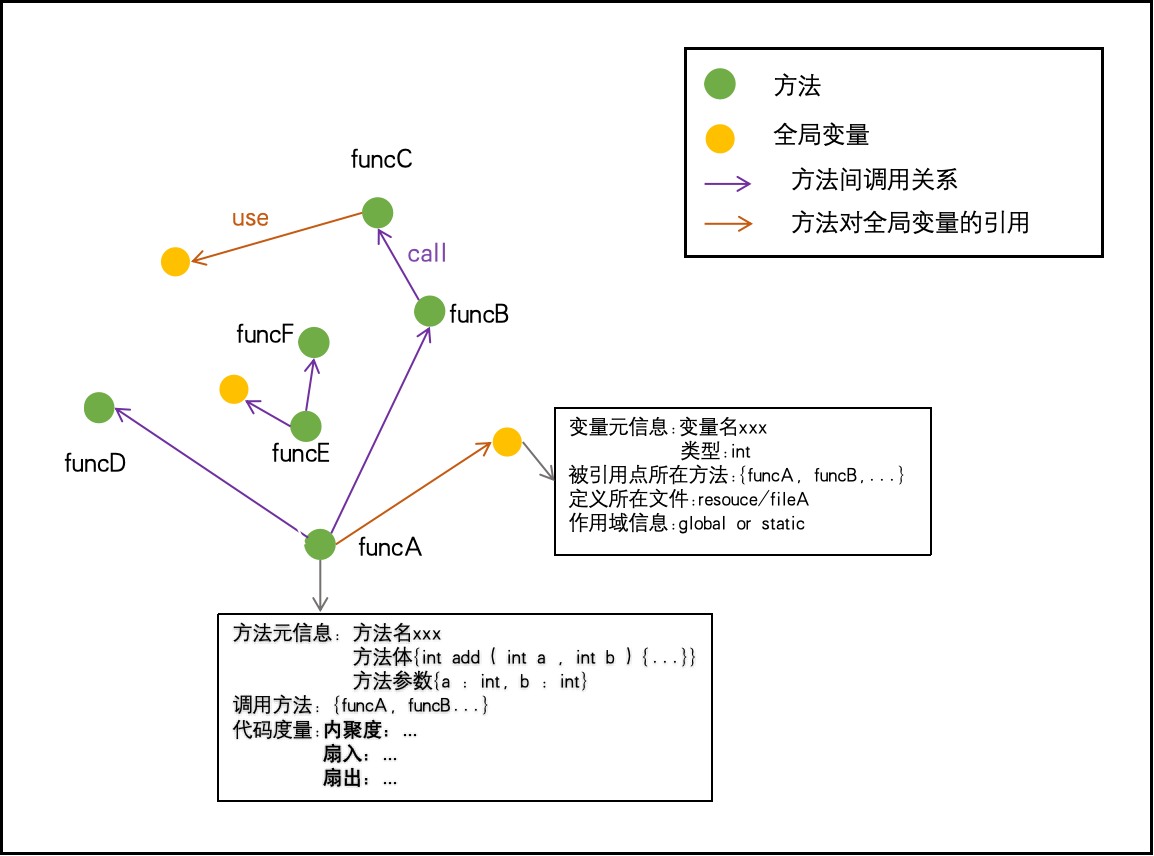
\includegraphics[width = 0.7\textwidth]{figures/依赖关系图.png}
    \caption{依赖关系图示例}
    \label{1_依赖图示例}
    \end{figure}


通过这种方式,依赖关系图不仅能够系统地表示代码中各个元素之间的直接依赖关系,还能为后续的变更影响分析提供结构化的图形模型。如图\ref{1_依赖图示例}为依赖关系图示例,该图中共有6个方法和3个全局变量,其静态依赖关系如图中的边所示。


\noindent \textbf{2. 执行变更影响分析}

这一过程旨在确定哪些方法在代码变更时可能受到影响,以及这些影响的传播路径。本文基于方法和方法之间的以下两种关系RBM(relationships between methods)对每一个方法识别当其变更时受影响的方法集IMS(impacted method set),定义如式\ref{1_RBM}所示,以方法f和方法g的关系为例,CALL方法和RETURN分别代表f和g的调用和被调用关系。
\begin{equation}
\begin{array}{l}
\label{1_RBM}
R B M=C A L L \cup R E T U R N \text { where } \\
(f, g) \in C A L L \Longleftrightarrow f(\text { transitively)calls } g, \\
(f, g) \in R E T U R N \Longleftrightarrow f(\text { transitively)returns into } g
\end{array}
\end{equation}

对于依赖关系图中的每个节点,计算该节点的传递闭包。传递闭包是指从某个特定节点出发,根据上文定义的依赖关系和图的可达性,可以直接或间接到达的所有节点的集合,反映了节点之间的依赖链以及影响传播的范围。传递闭包的具体迭代模型如下:
\begin{equation}
\begin{array}{l}
\label{1_IMS}
I M S^{(N)}=I M S_{C A L L}^{(N)} \cup I M S_{R E T U R N}^{(N)} \\
I M S_{ {RETURN }}^{(N+1)}=\bigcup_{define \in (I M S_{R E T U R N}^{(N)}-I M S_{R E T U R N}^{(N-1)} ) } I M S({ define }) \\
I M S_{C A L L}^{(N+1)}=\bigcup_{ {define } \in (I M S_{C A L L}^{(N)})} I M S( { define }){, define } \in \\
\left(I M S_{C A L L}^{(N)}-I M S_{C A L L}^{(N-1)}\right) 
\end{array}
\end{equation}


其中N表示第N轮迭代,第N+1轮的迭代受N和N-1轮的影响,反映出软件系统中的变更的涟漪效应。为了高效地计算传递闭包,使用广度优先搜索遍历图中的各个节点及其依赖边,进而识别出所有直接或间接依赖于某个节点的其他节点。每次从某个节点出发时,都会跟踪并记录通过依赖关系可到达的所有节点,,最终得到的节点集合中,所有的节点都与初始变更的节点存在某种直接或间接的依赖关系。这些方法可以视为受变更影响的范围,意味着它们在该方法变更后,可能会因为依赖关系的传递而受到影响。通过这一分析,我们不仅可以识别出受影响的直接方法,还能揭示出那些通过多次间接依赖而受到影响的方法,帮助开发者全面了解变更的潜在影响范围。


在图\ref{1_依赖图示例}的例子中,方法 funcA 调用了 funcB 和funcD,funcB 调用了 funcC。在对 funcB 进行变更影响分析时,会直接影响到 funcA和funcC,根据依赖关系闭包,会间接影响到funcD。所以与 funcB 有变更影响关系的方法集合为\{funcA, funcC, funcD\} 。


\section{基于克隆检测的变更影响分析}
代码克隆(Code Clone)是指在代码中存在两段或多段内容相似或完全相同的代码片段。因此它们在逻辑上往往具有相同的功能或行为。如果对其中一个克隆片段进行了变更(例如修复了一个 bug、添加功能或进行优化),那么在其他地方相同或相似的代码也可能需要同步修改,否则可能会导致系统的不一致性或错误,这是典型的逻辑型变更影响关系。

\begin{figure}[htbp]
\centering
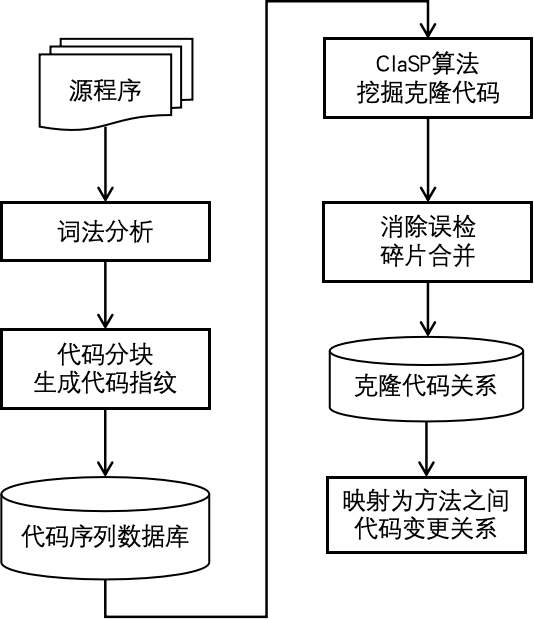
\includegraphics[width = 0.4\textwidth]{代码克隆流程}
\caption{基于克隆检测的变更影响分析方法流程}
\label{1_基于代码克隆的变更影响分析方法流程}
\end{figure}

因此,本文基于方法间的克隆关系进行变更影响分析。该方法主要分为两步,首先对源程序进行预处理,通过代码分段及代码指纹提取的方式对源程序进行编码,生成代码序列数据库。随后利用频繁模式挖掘算法ClaSP得到克隆代码列表,具体的处理流程如图\ref{1_基于代码克隆的变更影响分析方法流程}所示。



\subsection{代码预处理}

\paragraph{1. 词法分析} 这一步是拿到代码后的初步处理,主要有下面几步:

\begin{itemize}
    \item 去除注释:注释通常用于解释代码的意图,并不直接影响程序的执行,但不同的代码实现中注释内容可能存在差异,这会导致本质相同的代码片段由于注释的不同而被误判为非克隆。
    
    \item 去除头文件引用语句:源代码文件往往包含多个头文件,而不同的源文件可能引用相同的头文件。如果不对头文件进行统一的处理,算法就可能在不同的源文件中检测头文件引用的代码克隆情况,可能影响克隆检测的效率和准确性。
    
    \item 程序标准化:为了避免因变量名的变化导致漏检,在方法内部对变量名进行统一标准化处理。

\end{itemize}


\paragraph{2. 代码分块} 这一步将代码拆解成更小、更易于对比的单元,从而提高克隆检测的准确性。本文的代码分块策略按代码结构的不同分为几类:

\begin{itemize}
    \item 顺序结构:按固定行数分块,行数可由用户定义,默认为6行一块。行数越小则识别结果越精准,越能识别更细小的代码克隆情况。
    
    \item 控制结构:将选择结构(if、then、else、endif、switch)、循环结构(while、for)、和域结构(\{、\})共同描述为控制结构识别并根据关键分块词进行分块。这是由于控制语句是代码逻辑的重要分界点,将它们作为分块的标准可以确保检测系统能聚焦于实际功能的逻辑边界。
\end{itemize}

值得注意的是,分块时大括号不被视为代码块的一部分。不同的开发者在代码排版上可能存在差异,例如有的开发者将大括号置于同行,而另一些则习惯将大括号另起一行。为了避免这种格式差异对克隆检测结果产生干扰,大括号被排除在代码块之外。

\paragraph{3. 代码指纹提取} 遍历代码块的每一行语句,将每行语句转化为数字序列,再将所有数字序列合并,转化为代码块的“指纹”。该指纹将代表代码片段用于识别代码片段之间的相似性或重复性。鉴于哈希算法在计算上的高效性与实现的简便性,它在生成代码指纹方面具有显著的优势。因此,本文选择采用冲突率较低的hashpjw算法提取代码指纹。

\subsection{基于克隆检测的变更影响关系提取}
序列数据挖掘(Sequence Data Mining,SDM)是时序数据挖掘领域的一个重要研究方向,旨在从给定的输入数据库中,探索在大量对象之间随时间频繁出现的模式。判断一个模式是否具有意义的阈值被称为最小支持度。本文中,将代码指纹片段作为序列,合并起来为序列数据库,利用序列数据挖掘算法,挖掘频繁出现的模式,将问题转化为闭合序列挖掘问题。这里对于数据挖掘的一些基本概念不再赘述,具体可参考文献\cite{2013ClaSP}。

\paragraph{1. 基于闭合频繁子序列挖掘算法的代码克隆检测}主要分为两步,首先生成频繁序列,作为频繁闭合序列的候选FCC(Frequent Closed Candidates)。第二步执行剪枝,从候选中剔除所有非闭合的序列,最终得到精确的FCS(Frequent Closed Set)。主要的流程如算法\ref{1_ClaSP算法}所示,ClaSP算法由Gomariz等人\cite{2013ClaSP}提出,兼具高效性和准确性的优点。

\begin{algorithm}
\caption{ClaSP算法}
\label{1_ClaSP算法}
\KwIn{序列数据库}
\KwOut{频繁闭合序列集 $FCS$}
 $F_1 \gets \{\text{频繁 1-序列}\}$ \\
 $FCC \gets \emptyset$, $FCS \gets \emptyset$  \\
\For{\textnormal{all} $i \in F_1$}
{
    $F_{ie} \gets \{\text{频繁 1-序列的长大于i的扩展序列 } \}$ \\
    $FCC_i \gets \text{DFS-Pruning}(i, F_1, F_{ie})$ \\
    $FCC \gets FCC \cup FCC_i$
}

 $FCS \gets \text{N-ClosedStep}(FCC)$
\end{algorithm}


首先找到所有的频繁的1-序列(即长度为1的序列),然后,对于所有频繁的1序列,递归地探索相应的子树。对所有频率为1的序列进行此处理,得到FCC,最后,算法结束去除FCC中出现的非闭合序列。
    

DFS-Pruning 算法的通过递归生成候选模式(包括 s-扩展和 i-扩展,分别在模式末尾和任意位置添加新元素)并检查其支持度,最终返回以当前模式 $p$ 为前缀的所有频繁模式集。剪枝时,通过检查对应模式的子序列和超序列的支持度,将序列的节点进行合并,防止继续遍历冗余节点。最终得到的FCS即为所有克隆代码集。

\paragraph{2. 基于克隆代码碎片合并提取方法间的变更影响关系}

由于先前的代码分段处理导致克隆代码呈现为片段间的克隆关系,为了恢复代码的完整性,进一步对这些碎片进行合并。基于每段代码的位置信息,将属于同一方法的碎片进行合理整合,从而重建方法间的克隆关系。通过这种方式,最终得到的是方法与方法之间的克隆关系,反映了不同方法之间在代码修改过程中的潜在影响,即方法间的变更影响关系。

\section{基于共现关系挖掘的变更影响分析}

在软件工程中,分析代码变更历史是理解软件演化重要手段之一。在开发者对项目进行维护的过程中,通常是以一个提交(commit)为单位进行功能上的变更。当进入新的维护工作时,如对同一功能进行升级等,通常的做法是参考前人的开发历史,对当前开发工作做指导,以防止变更的不完全。基于这一特点,本文实现了基于变更历史和共现关联关系的变更影响分析方法,分析对象是软件项目的变更历史。该方法能够提取蕴含在代码变更历史中的变更影响关系,尤其适用于具有丰富变更记录的软件项目。

该方法的核心原理是在代码变更历史中,频繁同时更改的代码片段,通常存在着某种潜在的变更影响关系。这种变更影响关系不仅仅局限于静态结构上的依赖,还包括功能上的耦合和实现上的相互作用。因此,通过对这些历史变更数据的深入挖掘和分析,我们可以揭示出更丰富的逻辑型变更关系。

\noindent \textbf{1.基于代码变更历史提取的序列数据库构建}

由于 Git 是现代软件开发中最广泛使用的版本控制工具,因此,本文的分析主要基于由 Git 进行版本管理的项目。具体步骤如下:

\begin{itemize}
    \item 收集项目代码库及变更历史记录。克隆项目的代码库到本地,通过git log命令获取所有的commit,包括每个提交的哈希值commitHash等信息。
    \item 提取每个提交的变更信息。对每个提交运行git show <commitHash>命令,查看该提交引入的代码变更(即“diff”或差异),这会显示哪些文件被修改、添加或删除,本文主要关注标记为“修改”的文件,这些修改的文件中包含了具体的代码变化,即代码行的增、删、改操作,记录该commit引起的所有发生变更的代码行。
    \item 定位变更代码行所属的方法。定位变化代码行所在的方法。通过libclang分析变化前文件得到的抽象语法树可获取每个方法对应的代码行,与变更的代码行位置进行匹配,得到变更的代码行所在的方法。
    \item 提取变更方法与提交的关系。对于每个提交,提取出所有受影响的方法(即发生变化的方法),并将这些方法构成一个变更方法列表,用Map<commitID, List<Methods>>的结构存储每个commit变更的方法,作为序列数据库,便于后续分析与处理。
    
\end{itemize}

\noindent \textbf{2.基于共现关系挖掘的变更影响关系提取}

基于关联规则(Association Rules)的共现关系挖掘方法是反映事物之间相互依存性和关联性的一个重要数据挖掘技术,旨在从大量数据中挖掘出有价值的项之间的相关关系。共现关系可以视为关联规则的一种表现形式,它描述了在给定集合中,某一组项(或特征)经常出现在同一事务中。例如,在零售分析中,常见的共现关系是“购买了面包的顾客通常也会购买牛奶”。在这种情况下,“面包”和“牛奶”是一对共现项。在本文的代码变更影响分析中,共现关系描述的是在一次提交中,哪些方法经常同时发生变更。如果两个方法在多个提交中频繁一起变动,则它们之间可能存在某种依赖关系或变更影响关系。

\begin{algorithm}[h]
    \caption{频繁共现变更方法对挖掘算法}
    \label{同时变更方法对挖掘算法}
    \KwIn{序列数据库 $D$, 支持度阈值 $min\_sup$, 置信度阈值 $min\_conf$}
    \KwOut{变更影响方法对 $change\_impact\_pairs$}
     $F_1 \gets \emptyset$  \# 频繁1项集\\  
    \For{all $f \in D$} {
        \If{support$(f) \geq min\_sup$} {
            $F_1 \gets F_1 \cup f$
        }
    } 
    $F_2 \gets \emptyset$  \# 频繁2项集\\ 
    \For{all $(f_1, f_2) \in P = \{ (f_i, f_j) \mid f_i, f_j \in F_1, i \neq j \}$} {
        \If{$\text{Support}(f_1, f_2) \geq min\_sup$} {
            $F_2 \gets F_2 \cup (f_1, f_2)$
        }
    }
    
    $change\_impact\_pairs \gets \emptyset$ \\ 
    \For{all  $(f_1, f_2) \in F_2$} {
        \If{confidence$(f_1, f_2) \geq min\_conf$} {
            $change\_impact\_pairs \gets change\_impact\_pairs \cup (f_1, f_2)$
        }
    }
    \Return{$change\_impact\_pairs$}
    \end{algorithm}


常用的频繁项集的评估标准有支持度和置信度。支持度表示共现项在数据集中出现的次数占总数据集的比重,用于衡量一组项在数据集中的普遍程度。在代码变更分析中,支持度表示某一方法对在多个提交中同时出现的频率,计算公式如下:

\begin{equation}
\label{1_Support}
Support(funcA,funcB)=\frac{num(AB\text{共现})}{num(AllCommits)}
\end{equation}

置信度表示共现项中一个出现后,另一个项出现的概率。变更分析中,置信度度量表示当方法A被修改时,方法B被修改的概率,计算公式如下:

\begin{equation}
\label{1_Confidence}
Confidence(funcA\Leftarrow funcB)=\frac{P(AB\text{共现})}{P(B\text{出现})}
\end{equation}

在前文所述的基础上,本文设计了如算法\ref{同时变更方法对挖掘算法}所示的频繁共现变更方法对挖掘算法,算法的基本思想是通过挖掘在序列数据库中(即代码提交历史中)中的共现关系,计算得到频繁同时变更的方法对,这样的关系表明它们在变更过程中有着较为显著的相互依赖关系,反映了方法间的变更影响关系。

\section{基于代码预训练模型的变更影响预测}
\subsection{研究动机}

前文中所述的方法均有一定的局限性。

\begin{itemize}

    \item 冷启动问题:当项目代码拥有丰富的变更历史时,可以通过前文中介绍的共现关系挖掘方法,提取具有变更影响关系的方法对,然而并不是所有软件项目都有变更历史可供我们分析。

    \item 影响类型覆盖不全:在仅有项目源代码的情况下,共现关系挖掘方法无法直接应用,只使用基于依赖闭包和基于克隆检测的方法,则无法识别除这两种关系外的逻辑型变更影响。
    
    \item 影响模式难以迁移:共现关系挖掘方法仅能得到变更过的影响关系,对于未变更的方法,无法将相同的影响模式进行迁移。
    
\end{itemize}


因此本文提出基于代码预训练模型的变更影响预测方法,通过前面所述方法构建数据,并进行数据清洗,最后微调代码预训练模型来进行变更影响关系的预测,从而解决上述问题。

\subsection{数据集来源和数据清洗}
\label{1_数据集来源和数据清洗}
\paragraph{1. 数据集来源}

为了保证代码预训练模型能够识别依赖型和逻辑型两种影响关系,我们以依赖闭包,克隆检测,共现关系挖掘方法得到的影响关系作为原始数据。其中检测到有变更影响关系的方法对作为数据集的正例,通过对项目中的方法进行随机采样,从中选取一些不具有变更影响关系的方法对,作为数据集的负例。

\paragraph{2. 数据清洗}

依赖闭包,克隆检测,共现关系挖掘方法各自都会产生一些错误数据;依赖闭包找到的依赖方法对并不一定都有变更影响关系,共现关系挖掘置信度为1表示方法严格共现,但是支持度为2并不是十分严格的挖掘标准,因此数据集中会存在一些由于偶然共现导致的误报现象。为了排除此种样例,本文结合大语言模型对数据集进行清洗,以提高数据质量。


\begin{figure}[htbp]
\centering
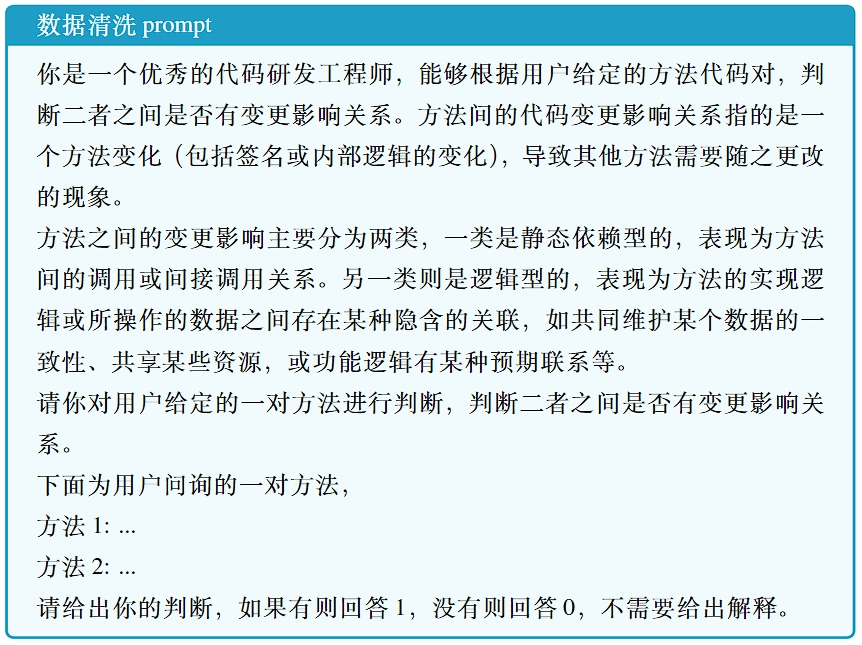
\includegraphics[width = 0.85\textwidth]{figures/1_数据清洗.png}
\caption{数据清洗所使用的的Prompt}
\label{1_数据清洗}
\end{figure}


现有商业大语言模型拥有较强的代码语义理解能力,能够对真实的变更影响关系进行精准识别,可以作为较好的数据清洗工具来使用。通过提示变更影响关系的类型以及对应的含义,能够帮助大语言模型对方法间的影响关系进行推理,从而排除掉误报样例,Prompt如图\ref{1_数据清洗}所示。


\subsection{基于代码预训练模型的变更影响关系预测}

基于代码预训练模型的影响关系预测任务的输入为两个方法体,输出为两个方法之间是否存在变更影响关系,即“存在”或“不存在”。

考虑到代码理解的复杂性与深度,相比于通用领域的如Bert,T5等预训练语言模型,面向代码领域进行预训练的CodeBert模型更适合作为编码器提取代码的表示。CodeBERT 是一种专为程序代码设计的预训练语言模型,通过大规模的代码语料库预训练,能够学习到代码中的丰富语法结构和语义信息。经过 CodeBERT 模型的表示学习,所得到的向量不仅包含了每个方法体的语法特征,还能够编码代码中的语义关系及其他潜在的编程特征。

我们的整个模型架构如图\ref{1_code_bert_overall}所示。
\vspace{0mm}
\begin{figure}[h]
\centering
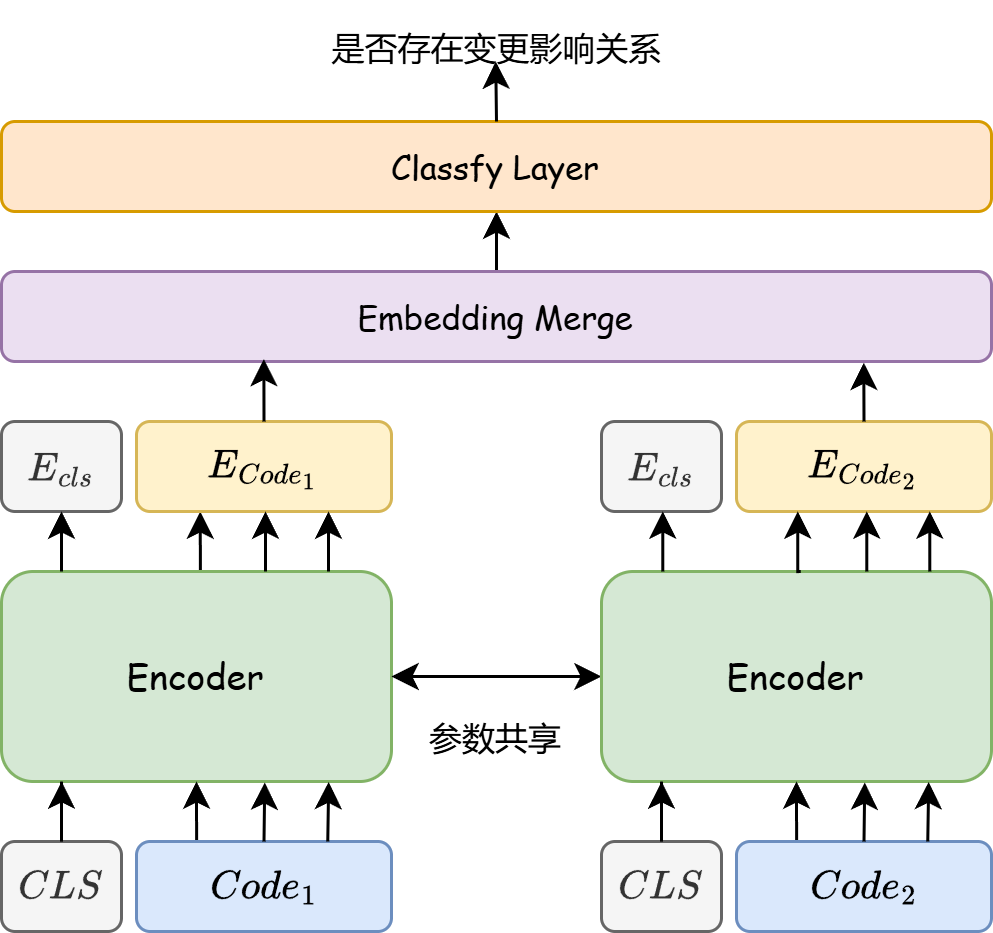
\includegraphics[width = 0.70\textwidth]{figures/1_code_bert_overall.png}
\caption{基于代码预训练模型的算法架构}
\label{1_code_bert_overall}
\end{figure}


首先,将两个方法体$ Code_1, Code_2$,先通过代码预训练模型进行编码
\begin{align}
H_{Code_1}=&Encoder(Code_1) \in \mathbb{R}^{(len,dim)} \\
E_{Code_1}=&mean(H_{Code_1}[1:...]) \in \mathbb{R}^{(dim)}
\end{align}

其中$len$表示$Code_1$的序列长度,$dim$为Encoder的隐层表示维度,得到方法的向量化表示$ E_{Code_1}, E_{Code_2}$。

通过拼接融合这两个向量,得到融合后向量表示$E_{Code_1,Code_2}$
\begin{align}
E_{Code_1,Code_2}=Concat& (E_{Code_1},E_{Code_1})\in \mathbb{R}^{(dim*2)} 
\end{align}

将融合后的向量表示送入一个由两层组成的多层感知机(Multilayer Perceptron,MLP)中,再通过 softmax 层进行分类处理,将模型的输出转化为一个概率分布,表示两个方法体之间存在关系的概率。
\begin{align}
logits_{Code_1,Code_2}=MLP(E_{Code_1,Code_2})&=FFN(ReLU(FFN(E_{Code_1,Code_2}))) \\
FFN(x)&=Wx+b\\
ReLu(x)&=max(0,x)\\
logits_{Code_1,Code_2}& \in \mathbb{R}^{(2)}
\end{align}

其中,$logits_{Code_1,Code_2}$为模型的MLP层最后给出的两种标签(存在关系,不存在关系)各自的概率。
\begin{align}
loss=CrossEntryLoss(logits_{Code_1,Code_2}, Label)
\end{align}

最后与真实标签$Label$计算交叉熵损失,得到loss,计算梯度,优化模型参数。


\section{实验结果与分析}

\subsection{实验数据}

\paragraph{1. 实验数据来源}

本文从影响力或社区活跃程度的角度出发,收集了表\ref{1_data_from}中所示的软件项目为被测项目进行实验。这些项目在github上的收藏数均在千以上,说明这些项目在开源社区中有着一定的影响力,使用范围比较广泛。除antiword项目之外,其他项目有着比较活跃的社区,说明其还在不断更新迭代过程中,所以能提供较为丰富的变更历史,以供共现关系挖掘方法的实验分析。

\begin{table}[htbp]
\caption{被测项目}
\label{1_data_from}
\vspace{0.5em}\centering\wuhao
\begin{tabular}{cp{6cm}ccc}
\toprule
项目名称 & 项目简介 & 代码行数& 提交数 & 收藏数 \\
\midrule
TheAlgorithms & 各种算法的开源实现,涵盖了计算机科学、数学和统计学等领域 & 24645 & 1536 & 57k \\
antiword-0.37 & 提取 Microsoft Word 文档内容的工具 & 34725& - & 13k\\
jemalloc-5.3.0 & 通用的malloc(3)实现,强调碎片避免和可扩展的并发支
持  &83525& 3530 & 9k \\
libbpf-1.1 & linux 内核观测技术的一个脚手架库 & 127927 & 2375 & 1.9k \\
librdkafka-2.1.0& Apache Kafka 的 C/C++ 客户端库 & 154951 & 4430 & 18k \\
FFmpegKit-5.1.0 & FFmpeg 工具包 & 450998 & 369 & 3.7k \\

\bottomrule
\end{tabular}
\end{table}


\paragraph{2. 训练数据}
基于代码预训练模型的变更影响预测方法的训练数据集收集方式如\ref{1_数据集来源和数据清洗}节所述,数据清洗过程中使用的模型为 Doubao (API model name:Doubao-lite-32k-240428),为了保证测试集和训练集的不重叠性,在经过收集和清洗后得到的关系中排除上述测试变更点。得到的训练数据统计信息如表\ref{1_数据集统计信息}所示,共12156对数据。

\begin{table}[htbp]
\caption{训练数据统计信息}
\label{1_数据集统计信息}
\vspace{0.5em}\centering\wuhao
\begin{tabular}{cccc}
\toprule
项目名称 & 正例对数 & 负例对数 & 总对数 \\
\midrule
TheAlgorithms    & 297 & 500 & 797 \\
antiword-0.37    & 230 & 500  & 730 \\
jemalloc-5.3.0   & 993 & 2000 & 2993 \\
libbpf-1.1       & 801 & 1500 & 2301 \\
librdkafka-2.1.0 & 1432  & 3000 & 4432 \\
FFmpegKit-5.1.0  & 303 & 600 & 903 \\ 
总计              & 4056 & 8100 & 12156 \\
\bottomrule
\end{tabular}
\end{table}


\paragraph{3. 测试数据}
根据每个示例项目的上一个版本和示例版本间的版本变更,分别各自选取30个变更方法,以代码变更记录作为辅助,以半手工的方式进行标注,得到真实的被影响方法集AIS(Actual Impact Set),作为测试集,这里分别统计了依赖型和逻辑型的变更影响关系,得到的数据如表\ref{1_test_data_info}所示。再分别通过前述方法进行检测,得到估计的被影响方法集EIS(Estimated Impact Set),通过评价指标评估方法的有效性。

\begin{table}[htbp]
\caption{测试数据统计信息}
\label{1_test_data_info}
\vspace{0.5em}\centering\wuhao
\begin{tabular}{cccccc}
\toprule
项目名称  & 变更点数 & 依赖型AIS & 逻辑型AIS & 总计 \\
\midrule
TheAlgorithms  & 30 & 98 & 21 & 119\\
antiword-0.37  & 30 & 119 & 54 & 173 \\
jemalloc-5.3.0   & 30 & 67 & 14 & 81 \\
libbpf-1.1  & 30 & 194 & 17 & 211 \\
librdkafka-2.1.0  & 30 & 92 & 26 & 118\\
FFmpegKit-5.1.0  & 30 & 105 & 17 & 122\\
总计  & 180 & 675 & 149 & 824 \\
\bottomrule
\end{tabular}
\end{table}


\subsection{评价指标}\label{1_评价指标}

真实的被影响方法表示为AIS,每种方法检测得到的结果为估计的被影响方法EIS,按逻辑型和依赖型对关系进行划分,根据这两个值计算精确度、召回率和F-measure,这三种评价指标在信息检索的场景下被广泛使用,本章中用于评价变更影响分析方法的有效性。
\begin{align}
precision &= \frac{|EIS \cap AIS|}{|EIS|} 
\end{align}

\begin{align}
recall &= \frac{|EIS \cap AIS|}{|AIS|}  
\end{align}

\begin{align}
F-measure &= \frac{2 \times precision \times recall}{precision + recall} 
\end{align}


\subsection{实验设置}

代码预训练模型选择:本文使用了CodeBERTa-small-v1和codebert-base-mlm两个模型分别作为代码表示模型,得到的代码表示为768维,融合两组表示后使用的多层MLP的维度为768*2,64,2。 骨干模型的学习率设置为1e-5,分类器的学习率设置为5e-4,优化器Adam的两个参数 $\beta_1$,$\beta_2$分别设置为0.95,0.999,batch\_size 为 64。数据收集过程中,共现关系挖掘方法置信度设为1,支持度设为2以获得较多的训练原始数据。

在实际训练过程中,由于CodeBERTa-small-v1和codebert-base-mlm模型都是类Bert模型,允许输入的上下文长度最大为512,但是经过统计数据集中有67\%的方法体在分词之后的Token数量是大于512的,所以本实验在实验中对于超长的方法体按照512进行分片,分片进行编码后对多组分片的$CLS$ token的表示进行平均,来作为方法体的编码表示。

我们的实验在 PyTorch 和 Transformer 库 上实现。CodeBERTa-small-v1和codebert-base-mlm均在单个 NVIDIA Tesla V100 GPU 上训练。


\subsection{实验结果与对比分析}

本节将通过实验对比来评估本章中提出的基于代码预训练模型的变更影响预测方法的性能,这里主要讨论下列三个问题:

RQ1:本章提出的基于代码预训练模型的方法能否有效检测变更影响关系?与其他方法相比,它在精确率,召回率和F-measure上表现如何?

RQ2:四种方法在提取依赖型(Dependence-Based)和逻辑型(Logic-Based)的变更影响关系上各自的优势如何?尤其是对于逻辑型的影响关系是否具有实际意义?分别适用于哪些特殊场景?又各自有怎样的局限性?

RQ3:基于代码预训练模型的方法的跨项目迁移表现如何?

\textbf{1.针对于RQ1的实验}

四种方法的实验结果如表\ref{1_变更影响实验结果}所示。


\begin{table}[htbp]
\caption{变更影响实验结果}
\label{1_变更影响实验结果}
\vspace{0.5em}\centering\wuhao
\begin{tabular}{cccccccc}
\toprule
方法 & F-measure & recall & precision  \\
\midrule
依赖闭包 & 36.8&81.9&23.7  \\
克隆检测 & 3.8&2.3&11.6 \\
共现关系挖掘 & 52.8&42.3&\textbf{70.4} \\
依赖$\cup$克隆$\cup$共现 & 47.1&\textbf{88.4}&32.1 \\
codebert-base-mlm & 58.8&53.9&64.8 \\
CodeBERTa-small-v1 & \textbf{59.5} & 55.3 & 64.4 \\
\bottomrule
\end{tabular}
\end{table}

通过对比可以发现,两个基于代码预训练模型的方法表现最好,其F-measure在所有方法中表现最优,并且在查全和查准的能力上较为平衡。这说明基于代码预训练模型的方法能够学习到过去变更历史中的行为模式,并能将学习到的变更关系知识进行迁移,用于判断新的影响关系。

其次基于共现关系挖掘的方法的准确率较高,但召回率略低。这表明,代码变更历史中方法的共现关系的确蕴含了大量能够有效揭示变更影响关系的信息。这是因为变更历史中都是前人对软件项目进行变更的记录,这样的提交由开发者精确变更,并经历过开源项目中非常严格的审查过程才合入主分支,因此较为准确地反映了代码变更中的实际操作,从而也能将过去的开发模式反映在共现关系挖掘的结果集中。


基于依赖闭包的方法表现为召回率较高而准确率很低,仅为23.7\%。这是由于依赖闭包方法本身的特性决定的,由于变更影响关系随涟漪扩散效应,越向外扩散影响越小,但该方法却平等地认为扩散所至的代码均存在影响关系,这并不不符合涟漪效应的特性。如在图\ref{1_依赖闭包方法迭代路径}中所示是antiword项目中从bTranslateImage方法出发得到的部分依赖图,它层层递进地展示了从word中提取jpec图片的过程,bTranslateImage调用bTranslateJPEG,处理jpec图片,再调用vASCII85EncodeFile,将图片提取为文件,再依次调用vASCII85EncodeArray和vASCII85EncodeByte。当对Byte方法进行变更影响分析时,根据RETURN关系的涟漪效应,最终会将图中所示的其他4个方法都列为影响集。然而实际上,该方法只对\{Array, File\}存在变更影响关系,最显然的,当Byte方法的签名发生改变时,将直接影响到\{Array, File\},这两个方法如果不更改将发生编译错误。而对另两种方法的影响则微乎其微。

\begin{figure}[htbp]
\centering
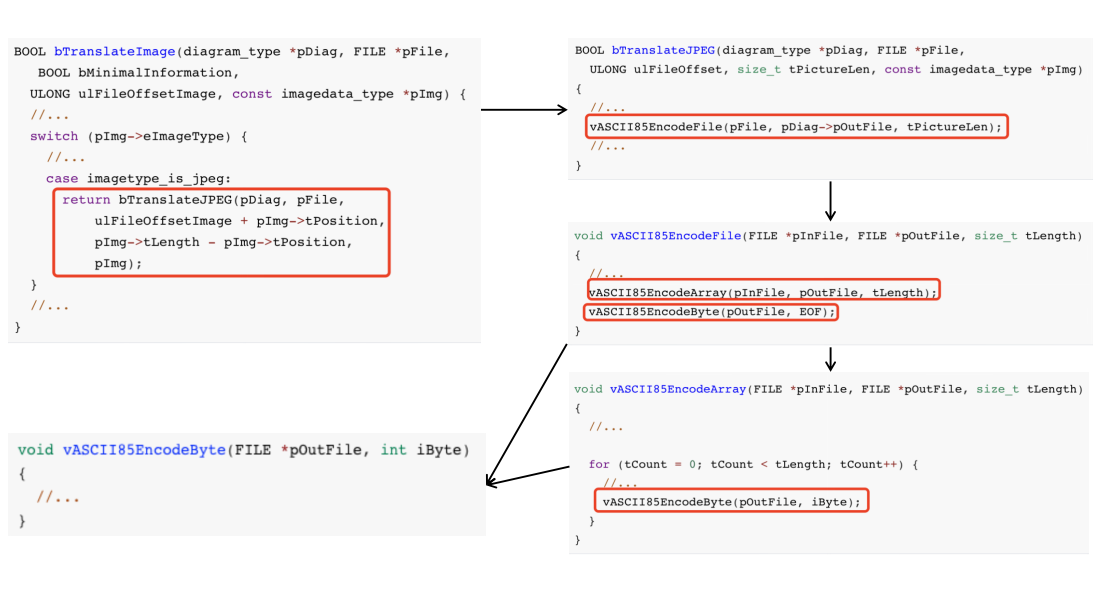
\includegraphics[width = 0.95\textwidth]{静态分析拒绝样例.jpg}
\caption{依赖闭包方法迭代路径}
\label{1_依赖闭包方法迭代路径}
\end{figure}


基于代码克隆检测的方法则整体效果最差。这是由于该方法只能准确的识别由于克隆关系产生的变更影响,而在质量良好的项目代码中,克隆代码的现象很少出现,因此提取到样例本身也较少,就导致其整体效果不佳。在实践中,建议基于克隆关系的方法作为其他方法的补充使用。

\textbf{2.针对于RQ2的实验}

RQ1中从整体的角度上说明了三种方法的有效性。为了回答RQ2,这里对每种方法检测得到的依赖型(Dependence-Based)和逻辑型(Logic-Based)的变更影响关系分别进行计算,得到如表\ref{1_两类变更影响关系实验结果}的结果。通过对两种类型分别的统计,我们能更直观地发现不同方法的优势和特点。


\begin{table}[htbp]
\caption{两类变更影响关系实验结果}
\label{1_两类变更影响关系实验结果}
\vspace{0.5em}\centering\wuhao
\begin{tabular}{c|ccc|ccc}
\toprule
  & \multicolumn{3}{c|}{Dependence-Based} & \multicolumn{3}{c}{Logic-Based}  \\
\midrule
方法 & F-measure & recall & precision & F-measure & recall & precision  \\
\midrule
依赖闭包 &  44.8 & 100 & 28.9 & - & - & -  \\
克隆检测 &  - & - & - & 31.8 & 19.1 & 95.7 \\
共现关系挖掘 &  56.0 & 44.6 & 75.4 & 57.0 & 47.3 & 71.8 \\
依赖$\cup$克隆$\cup$共现 &  44.1 & 100 & 28.3 & 62.3 & 53.7 & 74.1 \\
codebert-base-mlm &   61.2 & 55.1 & 68.9 & 70.9 & 72.6 & 69.3 \\
CodeBERTa-small-v1 &   \textbf{61.9} & 56.6 & 68.3 & \textbf{71.7} & 73.9 & 69.7 \\
\bottomrule
\end{tabular}
\end{table}


\paragraph{(1)依赖闭包方法} 对于依赖型影响没有漏报,但依赖型影响关系的误报较高,导致依赖型的检测表现整体上较差。针对逻辑型的变更,该方法则无法检测到,这是由于逻辑型的影响关系无法在依赖图中产生联系,因此依赖闭包方法无法检测。
    
\paragraph{(2)克隆检测方法} 逻辑型影响几乎没有误报,其准确率能达到95\%,说明其非常擅长挖掘逻辑型中由于克隆代码导致的变更影响关系。而这种关系在软件长期的维护中容易被忽略。但缺点在于仅能检测检测由于代码克隆导致的逻辑型影响,对于其他逻辑型和依赖型影响存在漏报。
    
以克隆检测方法挖掘到的一对有变更影响关系的方法为例,如图\ref{1_包含克隆代码片段的一组方法实例}所示。这里展示了这对方法的部分代码,其中绿色高亮的部分表示代码克隆的区域。这两个方法的主要功能是分别对8位和4位压缩格式的图像进行解码。我们发现,这对方法中的大部分逻辑结构几乎完全相同,只有少部分关键处理逻辑存在差异。由此,我们可以认定,这两个方法的变化过程很可能是同步的,即在实际的维护过程中,当对其中一个方法进行修改时,另一个方法也通常需要同步进行相应的变更,才能保证逻辑的一致性。

\begin{figure}[h]
\centering
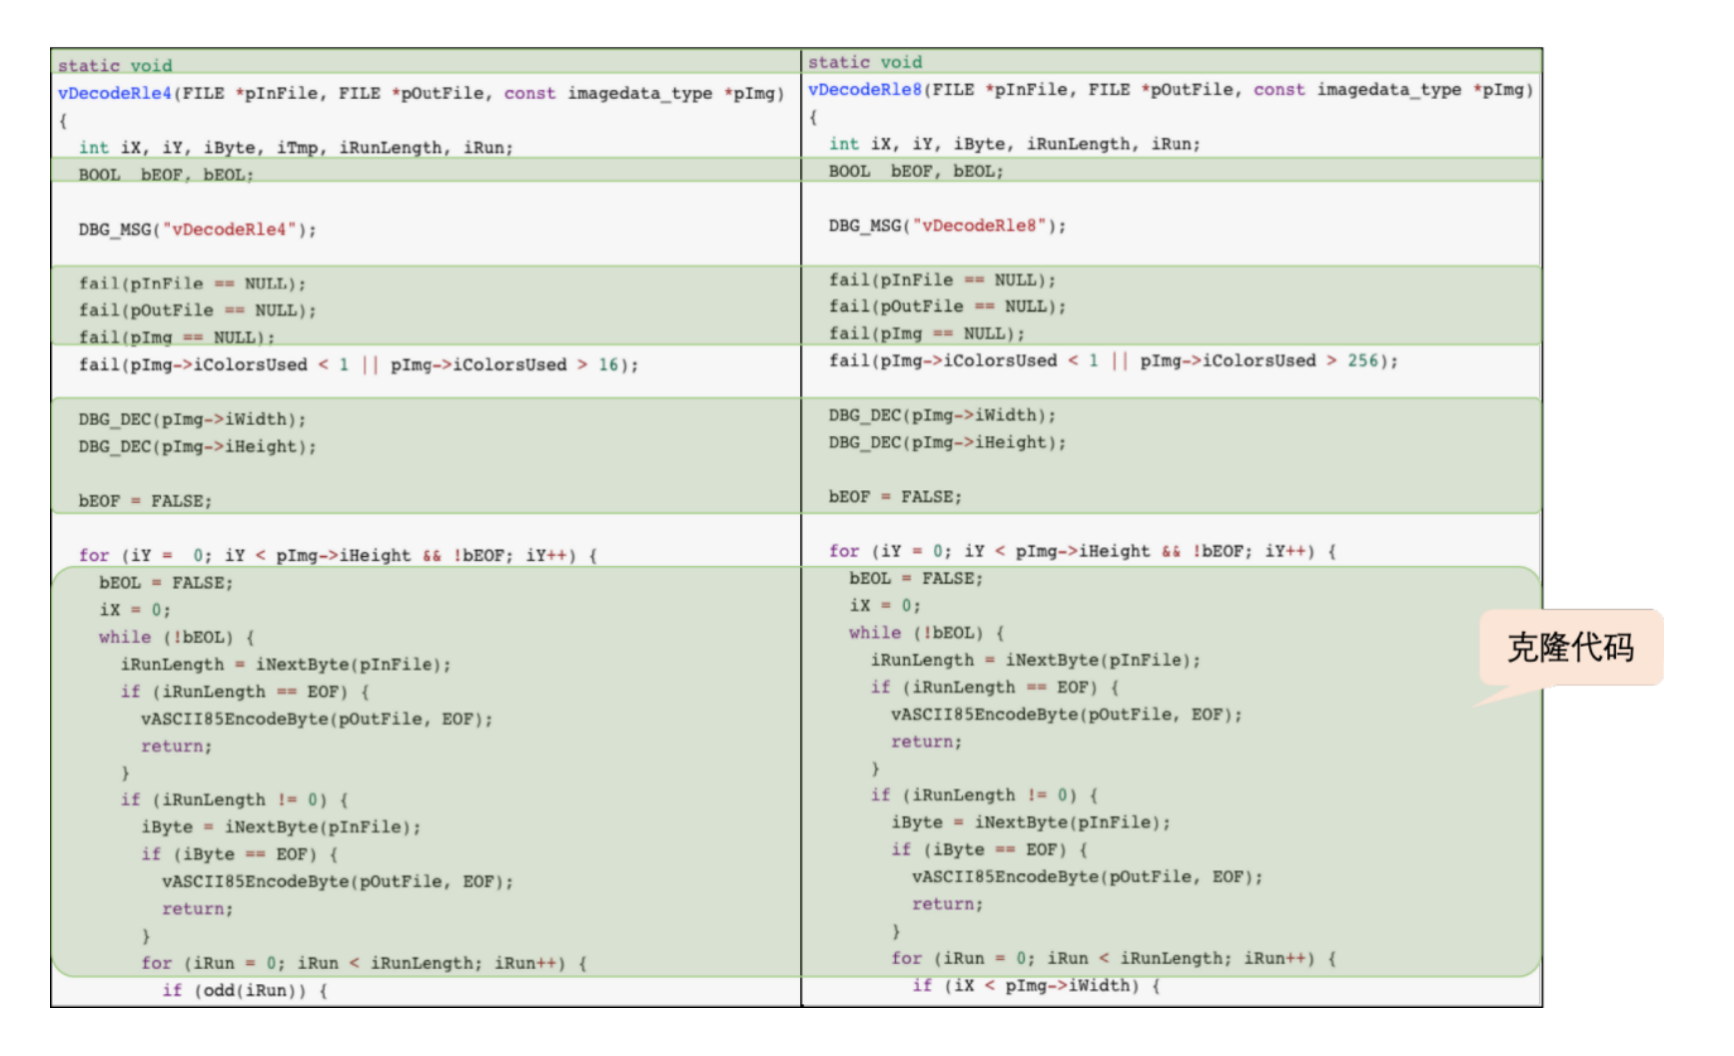
\includegraphics[width = 1\textwidth]{克隆代码示例.jpg}
\caption{包含克隆代码片段的一组方法实例}
\label{1_包含克隆代码片段的一组方法实例}
\end{figure}

这种现象表明,在软件的演化过程中,维护人员可能需要对这两个方法进行联动更新。任何对其中一个方法的修改都可能影响到另一个方法的功能或逻辑一致性,在代码维护时必须考虑它们之间的相互依赖关系。

\paragraph{(3)共现关系挖掘方法} 可以挖掘两种类型的变更影响关系。且在两类关系上的综合表现优于依赖闭包和克隆检测方法,说明其在使用场景中是更实用的一个方法,并没有前两种方法非常极端的倾向。但该方法也存在一定局限性:(1)要求项目代码必须有变更历史。(2)挖掘算法的支持度对结果有影响。表\ref{1_支持度对共现关系挖掘方法的影响}是支持度分别为2和3对应的实验结果。可以发现,支持度越大,误报越少,但是漏报越多。这说明支持度越大越排除了一些变更共现的偶然因素,但是失去了对影响关系的普遍性检测,能检测出的关系更少,导致了漏报增加。(3)挖掘到的信息属于硬信息。仅依靠变更历史的只能得到变更过的方法之间影响,未变更过或变更次数较少的影响关系无法反映,相同的影响模式之间无法进行迁移。
        
\begin{table}[htbp]
\caption{支持度对共现关系挖掘方法的影响}
\label{1_支持度对共现关系挖掘方法的影响}
\vspace{0.5em}\centering\wuhao
\begin{tabular}{c|ccc|ccc}
\toprule
  & \multicolumn{3}{c|}{Dependence-Based} & \multicolumn{3}{c}{Logic-Based}  \\
\midrule
方法 & F-measure & recall & precision & F-measure & recall & precision  \\
\midrule
共现关系挖掘-支持度-2 & 55.5 & \textbf{51.2} & 60.7 & 56.1 & \textbf{58.9} & 53.5 \\
共现关系挖掘-支持度-3 & \textbf{56.0} & 44.6 & \textbf{75.4} & \textbf{57.0} & 47.3 & \textbf{71.8} \\
\bottomrule
\end{tabular}
\end{table}
   
以共现关系挖掘方法在 librdkafka 项目中挖掘到的一对方法为例,如图 \ref{1_逻辑上有变更影响关系的方法对示例-incr和decr} 所示,该项目是 Apache Kafka 的一个高性能 C/C++ 客户端库,左侧的方法rd\_kafka\_global\_cnt\_decr负责对计数器进行减一操作,而右侧的方法rd\_kafka\_global\_cnt\_incr则负责对计数器进行加一操作。

\begin{figure}[h]
\centering
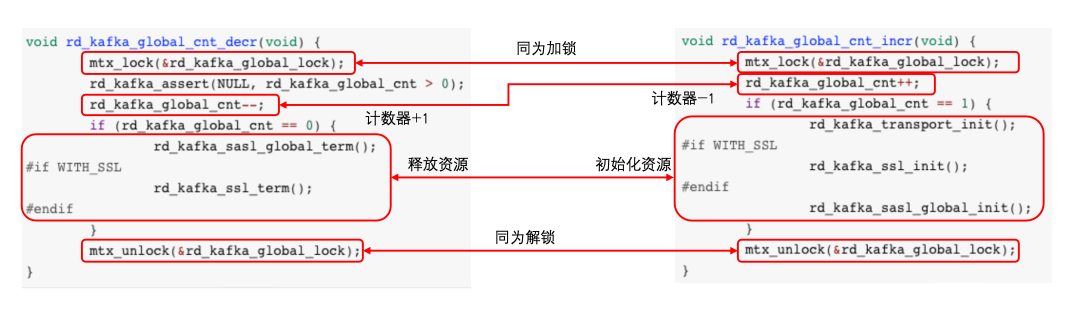
\includegraphics[width = 1\textwidth]{incrdec.jpg}
\caption{逻辑上有变更影响关系的方法对示例-incr和decr}
\label{1_逻辑上有变更影响关系的方法对示例-incr和decr}
\end{figure}

从功能上来看,这两个方法是一对典型的协作方法,其作用密切相关。具体来说,incr方法执行计数器加一操作,在计数器从零变为一时,执行资源的初始化工作。而 decr方法则在计数器减为零时,执行资源的释放操作。从代码实现可以看出,这两个方法的操作逻辑具有明显的互补性,加一与减一、初始化与释放的功能关系呈现出“镜像”特性。

尽管它们依赖图上无法产生联系,但由于它们在功能上承担了计数器的管理和资源的初始化与释放工作,其逻辑关联性非常强。因此,当其中一个方法的实现逻辑发生变化时,另一个方法通常需要进行相应的调整,以保持整体逻辑的一致性,这种方法对的变更影响关系属于典型的逻辑关联型变更影响关系。

\paragraph{(4)代码预训练模型}

该方法在两类变更影响关系上的表现均达到最优,与之前的方法相比,在两类变更影响关系上的F-measure分别提升了5.9\%和14.7\%。此外,该方法有效解决了共现关系挖掘方法在缺乏变更历史时的冷启动问题,且在逻辑型影响的挖掘上能够实现影响模式的迁移。然而,在依赖型影响的挖掘上,也展现出了比较均衡的效果,但是F-measure的提升稍显逊色,可能的原因在于多跳依赖的两种方法体之间在语义层面的关联性较难识别,从而导致对这种类型依赖关系的识别能力较弱。

由于该方法引入了代码预训练模型,在使用中计算量会显著增大。以antiword项目为例,该项目中共有578个方法体,测试集中的变更点为30个。对于每一个变更点,都需要与项目中的所有方法进行一一比对,计算的次数为30 * (577) = 17,310次,每次计算均需要通过嵌入和分类过程。大量的计算时间消耗显著影响了该方法的可用性,从而限制了其在大规模项目中的应用效果。
    

\textbf{3.针对于RQ3的实验}

为了探索基于代码预训练模型在跨项目方面的迁移能力,本节对实验所使用到的六个数据集进行划分,将TheAlgorithms,antiword-0.37,librdkafka-2.1.0和FFmpegKit-5.1.0划分为训练集,我们将这四个代码库称为分布内代码库,将jemalloc-5.3.0和libbpf-1.1划分为测试集,我们将这两个代码库称为分布外代码库;以保证训练集和测试集的数据来源没有交集;更符合应用时的场景设置,即在使用时可能会遇到训练中从未见过的代码库。


\begin{table}[htbp]
\caption{跨项目迁移能力分析(F-measure)}
\label{1_跨项目迁移能力分析}
\vspace{0.5em}\centering\wuhao
\begin{tabular}{c|cccc|cc}
\toprule
方法& TheAlgorithms & antiword & librdkafka & FFmpegKit & jemalloc & libbpf\\
\midrule
train on 6 datasets & train & train & train & train & train & train \\
\midrule
codebert-base-mlm &  59.66 & 60.43 & 57.47 & 57.03 & 59.67 & 57.82\\
CodeBERTa-small-v1 &  60.23 & 59.64 & 60.18 & 57.87 & 60.99 & 58.22\\
\midrule
train on 4 datasets & train & train & train & train & test & test \\
\midrule
codebert-base-mlm &   61.72 & 61.55 & 62.03 & 60.65 & 42.49$^*$ & 39.75$^*$ \\
CodeBERTa-small-v1 &  62.28 & 65.24 & 63.45 & 62.19 & 41.92$^*$ & 40.8$^*$\\
\bottomrule
\end{tabular}
\end{table}

实验结果如表\ref{1_跨项目迁移能力分析}所示,仅在分布内代码库上进行训练的模型,在对应测试集上的表现会略有提升,并且在分布外代码库的测试集上也能有一定的性能迁移,但相比在六个数据集上进行训练的模型,性能下降在28.9\% 到 31.7\%之间。

\textbf{4.方法对比总结}

上述四种方法为检测代码变更影响关系提供了多样化的解决方案。每种方法在处理不同类型的变更影响关系时各有侧重,适应于不同的应用场景。然而每种方法也存在一定的局限性。对于这些方法的比较与总结,请参见表\ref{1_变更影响分析方法对比总结}。


\begin{table}[htbp]
\caption{变更影响分析方法对比总结}
\label{1_变更影响分析方法对比总结}
\vspace{0.5em}\centering\wuhao
\begin{tabular}{c|c|p{4cm}|p{4cm}}
\toprule
方法& 检测关系 & 优势 & 局限性\\
\midrule
依赖闭包 & 依赖型 & 依赖型漏报低 & 依赖型误报高,且仅能检测依赖型\\
\midrule
克隆检测 & 逻辑型-代码克隆 & 逻辑型中克隆关系影响的误报低 & 只能检测代码克隆一种关系\\
\midrule
共现关系挖掘  & 依赖型和逻辑型 & 两类影响的性能均较好 & 无法应用于没有变更历史的项目,不频繁变更无法被检测 \\
\midrule
代码预训练模型  & 依赖型和逻辑型 & 两类影响的性能均较好 & 计算效率问题 \\
\bottomrule
\end{tabular}
\end{table}



\section{本章小结}

本章实现了基于依赖闭包、克隆检测、共现关系挖掘的变更影响分析方法,并提出了基于代码预训练模型的变更影响预测方法。通过实验分析了基于依赖闭包、克隆检测、共现关系挖掘的三种方法的优势以及局限性,实验中基于代码预训练模型的变更影响预测方法在两大类关系的检测中均表现出了最优的性能,并且各个指标上没有明显缺陷,但是由于其对计算量的要求较高,所以在实际场景中的应用价值会有一定程度的折扣。

% Local Variables:
% TeX-master: "../main"
% TeX-engine: xetex
% End:

%%%%%%%%%%%%%%%%%%%%%%%%%%%%%%%%%%%%%%%%%%%%%%%%%%%%%%%%%%%%%%%%%%%%%%%%%%%%%%%
\chapter{基于代码依赖与检索增强生成的代码变更影响分析}

\section{引言}

% 在软件系统的开发周期中,随着整体架构的日益复杂以及规模逐渐扩大,程序员在进行功能迭代、Bug修复等任务时,往往会面临较大的挑战。尤其是在庞大的代码库中,程序员难以快速且高效地评估某一变更对整体系统的影响。因此,若能在工作中引入一种高效的系统或算法来自动化地分析代码变更所带来的潜在影响,将极大地提升程序维护人员的工作效率。这不仅有助于减少潜在漏洞的发生,也能够确保系统在不断演进的过程中保持高质量和稳定性。由此可见,代码变更影响分析成为了软件开发中一个亟待关注的关键问题,值得深入研究与探讨。

由于代码预训练模型优秀的泛化能力和知识迁移能力,第二章中基于代码预训练模型的变更影响分析方法相较于基于方法间关系的方法具有更优秀的性能。但是由于其计算效率问题,导致其在实际使用时较为耗时。除此之外,由于该方法仅靠两两方法体的代码进行变更影响关系的检测,因此方法代码中无法反映的间接依赖信息在检测时缺失了,导致其在间接依赖的影响关系判断上表现不好。

检索增强生成(Retrieval Augmented Generation,RAG)技术由Lewis 等人\cite{2020Retrieval}于 2020 年提出,是一种将信息检索与生成式模型(如 GPT 等)相结合的技术,它可以在文本生成过程中有效利用外部知识库或数据库中的信息,以提高生成结果的准确性和上下文相关性。RAG工作流程可以概括为两步,检索和生成。检索过程中根据输入问询(query),从外部知识库(如文档库、网页、数据库)中检索与输入相关的上下文或片段,生成阶段将检索到的信息与用户的输入结合起来,作为生成模型的输入,生成模型根据检索的上下文生成答案或内容。RAG方法能有效解决端到端问答模型的效率问题和减少事实错误的发生。

为了进一步提升代码变更影响分析的效率和可用性,本章提出了一种基于代码依赖与检索增强生成的代码变更影响分析算法。本方法以代码库中的海量方法体为知识库,通过信息检索技术,生成候选方法集合,如果候选方法中有与变更方法存在间接依赖关系的方法,则根据代码依赖图提取调用路径上的中间方法,构造推理信息。利用当前大规模语言模型在各种文本领域上强大的语义理解和生成能力,准确的判断候选集合中的变更影响关系。

在该算法中,信息检索模块能够显著降低计算时间,确保在大规模代码库中快速定位相关代码,通过提供调用路径的中间方法,保证模型判断时的代码逻辑的完整性,而大语言模型部分则保证了变更影响关系分析结果的高准确性。此外,通过动态调整候选集合的大小,可以有效平衡算法的运行速度与分析效果,从而使得整个系统既高效又可靠,能够在实践中为程序维护和优化提供有力支持。

\section{研究动机}

上一章节所提出的基于代码预训练模型的变更影响分析方法,尽管在测试基准方面取得了当前最优的效果,然而,其仍然存在两个较为显著的问题,即计算效率问题和间接依赖的语义缺失问题。

\textbf{计算效率问题:}每当需要针对代码库中的一个变更点展开变更影响分析时,都必须将变更方法体与整个代码库的其他方法体组对,然后输入模型进行检测。对于规模较大的项目代码而言,这种方法所带来的计算延迟会严重影响其可用性,几乎使其无法正常使用。

针对该问题,可以考虑将对方法体的编码与变更关系的分析两个阶段进行解耦。在初始化阶段,运用嵌入模型对代码库的全部方法体进行编码并存储。当需要对某个变更点进行分析时,仅需通过向量相似度计算筛选出少量候选方法,利用大语言模型优越的语义理解能力进行其变更影响关系的判断。

\textbf{间接依赖的语义缺失问题:}由于基于代码预训练模型的算法仅依据两个方法体的代码来判断变更影响关系,因此当两个方法体之间存在间接依赖时,如果不提供中间方法的调用逻辑,相关信息便会缺失,这将导致模型无法合理推断方法之间的变更影响关系。在这种情况下,只有资深工程师凭借对方法功能的了解,结合丰富的经验才能够完成判断,但即便如此,也很难保证判断的正确性。

针对该问题,可以考虑在判断间接依赖的方法体之间的变更影响关系时,提供其调用路径中的中间方法,补全缺失信息,以便为模型提供支持,实现准确的判断。

因此,本章提出了基于代码依赖与检索增强生成的代码变更影响分析技术。该技术借助检索方式和代码依赖图,分别解决计算效率问题以及间接依赖所带来的语义缺失问题,从而提升变更影响分析在实际应用中的效果。


\section{基于代码依赖与检索增强生成的变更影响分析方法}


\subsection{整体流程设计}

为了解决第二章中基于代码预训练模型方法的计算效率问题与间接依赖语义缺失问题,本章提出了基于代码依赖与检索增强生成的变更影响分析方法。图\ref{2_基于代码依赖与检索增强生成的变更影响分析方法框架}中展示了本章方法的研究框架。本章的方法主要流程分为三个阶段:

\begin{enumerate}

    \item \textit{数据构建;}主要需要构建两个部分的数据:(1)代码依赖图。构建完整代码库以方法为粒度的代码依赖图,以支持后续间接调用的检测与查询。(2)嵌入模型训练需要的三元组语料。将完整代码库按照方法的粒度进行切分并作为知识库;以上一章节的依赖闭包、克隆检测、共现关系挖掘三种方法检测出的变更影响关系为原始数据,基于大预言模型与代码依赖图进行数据清洗,构建准确的变更影响关系方法三元组(查询,正例,负例),用于训练嵌入模型,使嵌入模型专精于检测变更影响关系这一垂直领域。

    \item \textit{检索模块;}在三元组语料上训练嵌入模型,并使用嵌入模型对知识库进行预编码。在测试时仅需对查询方法进行编码,并与知识库中的向量计算相似度,找出相似度最高的前$k$个(top-$k$)作为候选方法。
    
    \item \textit{增强生成;}构建由变更点方法,候选方法集合,调用路径的中间方法(如有)组合成的提示,使用大语言模型对候选方法进行判断,得到最终的有变更影响关系的方法。
    
\end{enumerate}

\begin{figure}[htbp]
\centering
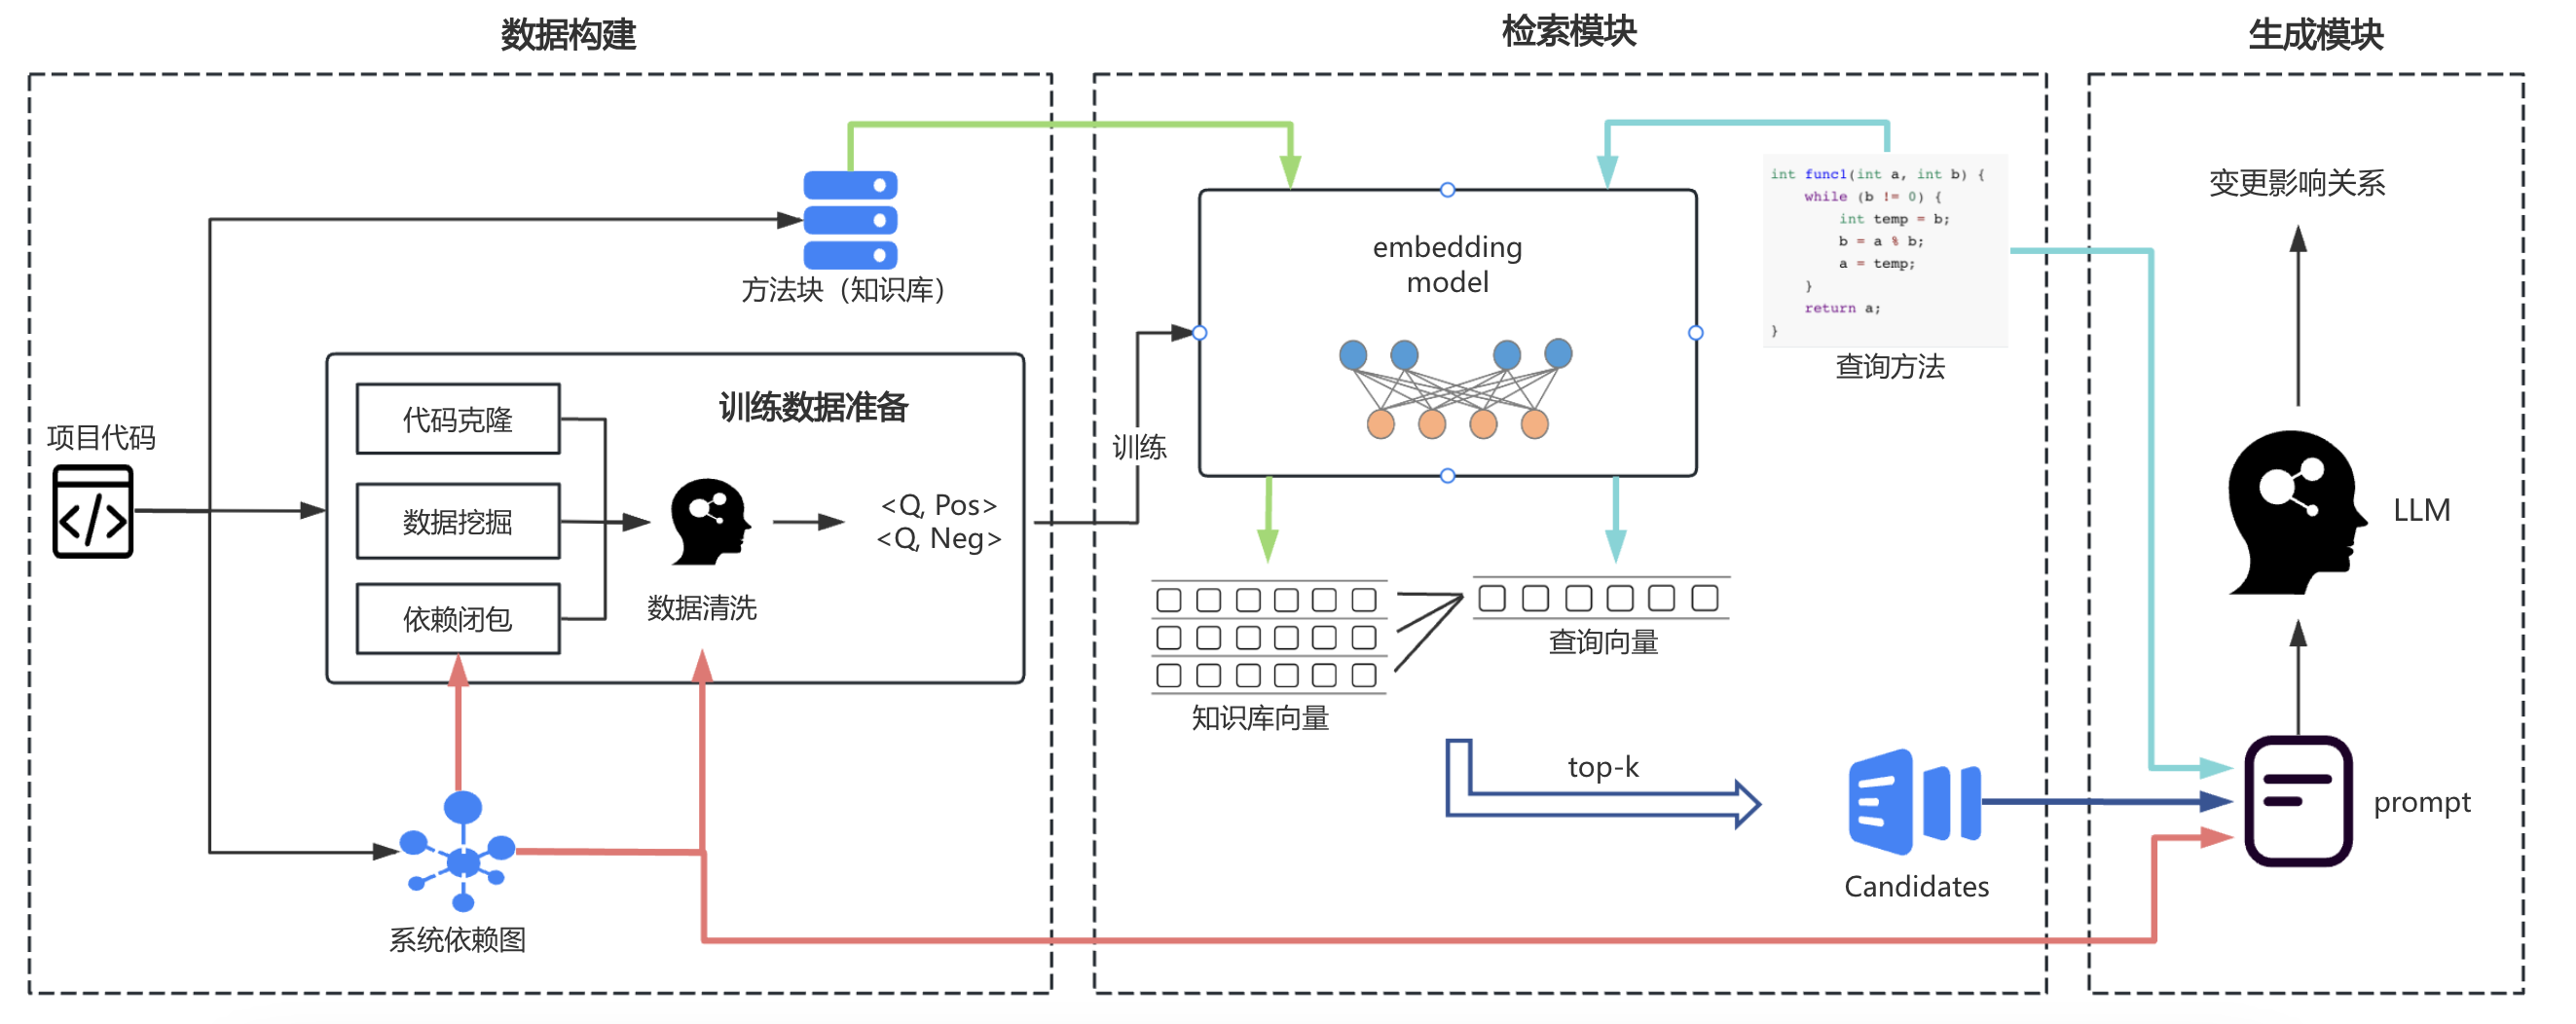
\includegraphics[width = 1\textwidth]{RAG架构.jpg}
\caption{基于代码依赖与检索增强生成的变更影响分析方法框架}
\label{2_基于代码依赖与检索增强生成的变更影响分析方法框架}
\end{figure}


\subsection{数据构建}


\paragraph{1. 代码依赖图构建} 对被分析的整个代码库按照方法的粒度进行切分,根据章节\ref{1_代码依赖图}所述,构建以方法体为顶点,以调用关系为边的代码依赖图。

\paragraph{2. 嵌入模型训练数据构建} 为了让检索模块对变更影响关系的召回率足够高,需要对嵌入模型进行训练,使具有变更影响关系的方法在向量空间中更接近,因此需要构建嵌入模型的训练数据。我们以上一章节的依赖闭包、克隆检测、共现关系挖掘三种方法检测出的变更影响关系为原始数据,使用大语言模型进行数据清洗,以得到足够准确的正例对,并对正例对中任选其一在项目中随机采样得到对应的负例,得到训练嵌入模型所需的$<Query,Pos,Neg>$三元组数据。

假设上一章节的依赖闭包、克隆检测、共现关系挖掘三种方法检测出的变更影响关系对集合为$S_{raw}$,其中$<Code_i,Code_j>\in S_{raw}$,参考上一章节的实验部分可知,$S_{raw}$中存在部分误报关系,如果不加处理,会严重影响检索模块的性能。

在对$S_{raw}$进行数据清洗时,由于在前文中提到,深度学习方法对于间接依赖导致的变更影响关系检测效果较差,正是由于方法间的间接调用信息存在缺失导致的。由此我们考虑结合依赖路径进行数据清洗。对于每一对$<Code_i,Code_j>$,数据清洗流程如下:


(1)判断依赖可达性;根据代码依赖图判断两个方法体之间是否存在调用关系,如果是直接调用,则无需处理;如果是间接调用,则需要补充调用路径的中间方法为$<Code_i,Code_{mid_1},Code_{mid_2},Code_j>$。

(2)基于大模型进行变更影响关系判断;利用代码能力与语言理解能力出色的大预言模型,为原始数据$S_{raw}$中的每一组数据构建如下图\ref{2_数据清洗prompt}的提示,进行变更影响关系的判断,剔除大模型认为没有变更影响关系的数据,剩下的数据整合为$S_{filtrate}$,其中$<Code_i,Code_j>\in S_{filtrate}$。

\begin{figure}[htbp]
\centering
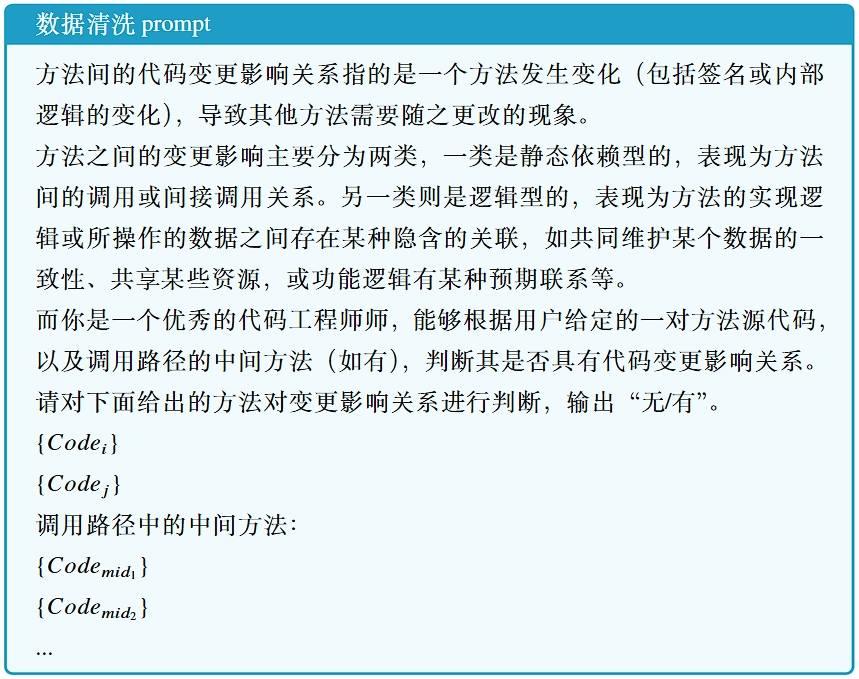
\includegraphics[width = 0.85\textwidth]{figures/2_数据清洗prompt.png}
\caption{数据清洗所使用的的Prompt}
\label{2_数据清洗prompt}
\end{figure}


接下来为$S_{filtrate}$中的数据采样负例,对于每组数据$<Code_i,Code_j>$,随机挑选其中一个方法作为查询$Code_{query}$,另一方法作为正例$Code_{pos}$统计$S_{filtrate}$中出现的$Code_{query}$的正例集合 $\{Code_{pos},Code_k,Code_e,Code_k,\}$,从代码库中除正例集合之外的方法中随机采样方法作为负例$Code_{neg}$,将构建好的三元组数据$<Code_{query},Code_{pos},Code_{neg}>\in S$作为嵌入模型的训练数据,我们之后简写为$<Query,Pos,Neg>$。

\subsection{检索模块}

检索模块主要分为离线和在线两个阶段。

离线阶段的主要任务是完成嵌入模型的训练,并对知识库中每个方法体进行嵌入。具体而言,嵌入模型通过对代码库中的每个方法进行编码,将其转换为具有语义信息的稠密向量表示。这些嵌入向量随后被存储在知识库中,为后续的检索任务提供基础。

在线阶段则针对每个查询进行实时处理。首先,通过嵌入模型将查询内容转化为稠密向量表示。然后,基于该查询向量与知识库中已嵌入方法体的向量进行相似度计算。最后,按照相似度排名从知识库中选出Topk个与查询向量相似度最高的方法体,作为疑似具有变更影响关系的候选方法。

\paragraph{1. 嵌入模型的训练}

嵌入模型通常用于将文本数据这种长度不一、非对齐的形式转换为固定长度的稠密向量表示。具体来说,对于一段文本数据$text={t_1, t_2, ..., t_n}$。对于训练数据中的三元组数据的嵌入$<E_{Query},E_{Pos},E_{Neg}>$,因为其用途一般是为了完成高效的检索,因此训练目标与使用场景相对应,希望达到的效果是将$E_{Query}$与$E_{Pos}$的相似度尽可能地提高,将$E_{Query}$与$E_{Neg}$的相似度尽可能地降低。在实际训练是经常使用对比损失函数 InfoNCE Loss 进行训练:

为了实现这一目标,通常采用对比损失函数(Contrastive Loss),其中InfoNCE Loss是一种常用的选择。其定义为:

\begin{equation}
    L_{InfoNCE} = -\log\frac{\exp(sim(E_{Query}, E_{Pos}) / \tau)}{\exp(sim(E_{Query}, E_{Pos}) / \tau)+\exp(sim(E_{Query}, E_{Neg}) / \tau)}
\end{equation}

其中,$\tau$为温度因子,用于控制相似度的平滑程度。通过最小化$L_{InfoNCE}$来优化嵌入模型,从而提升查询向量与正样本之间的相似度,同时减少与负样本之间的相似度。

为了与后续在线相似度计算的工程实现相匹配,本文在相似度度量上选择了欧式距离(L2距离):

\begin{align}
sim(A,B)&=-L2(A, B)  = -\sqrt{\sum_{i=1}^{n} (y_i - x_i)^2} \\
A &= (x_1, x_2, \dots, x_n) \\
B &= (y_1, y_2, \dots, y_n)
\end{align}

\paragraph{2. 知识库的构建}

在训练出嵌入模型后,为了在实际应用中提升推理速度,必须基于完整的代码库构建一个知识库。这一过程旨在将代码库中的每个方法体转换为具有语义信息的稠密向量表示,从而便于在推理过程中高效地进行检索。具体而言,使用前一章节中训练得到的嵌入模型对代码库中的每个方法体$Code_i$进行编码,得到对应的向量表示$E_{Code_i}=Embedding\_model(Code_i)$,其中每个$E_{Code_i}$是一个包含该方法语义信息的稠密向量。经过编码后,所有方法体的向量集合为$\mathbf{E}={E_{code_1}, E_{code_2}, ..., E_{code_n}}$,其中$n$表示代码库中方法体的总数。

为了提高知识库检索的效率,本研究采用了FAISS(Facebook AI Similarity Search)作为稠密向量的检索工具。FAISS是一种高效的向量检索框架,能够对大规模向量数据进行索引并支持快速检索。通过构建向量索引,FAISS能够显著提高在大规模数据库中进行相似度搜索的速度。FAISS支持多种类型的索引结构,包括平坦索引、倒排文件索引和层次化导航图等,这些索引结构能够根据数据的规模、向量维度及存储需求,灵活应对不同查询速度和精度的需求。

鉴于本文的研究对象是软件项目代码,且分析粒度为方法级别,代码库中的方法数量通常较少,最多只有几千个方法。与处理文档类问答生成任务中涉及的大规模数据集不同,本文的代码库规模相对较小。因此,在构建索引时,本文选择了较为简单的平坦索引结构对方法向量进行检索。

\paragraph{3. 查询的嵌入}

在实际使用中,到达一个新的查询$Query$,使用上文经过训练的嵌入模型进行嵌入$E_{Query}=Embedding\_model(Query)$;

\paragraph{4. 知识库的检索}

在获得查询的嵌入表示$E_{Query}$之后,便可以利用FAISS对知识库中的向量进行检索,选择与查询向量$E_{Query}$在L2距离上最为接近的$k$个向量。通过这些相似度最高的$k$个向量的索引,可以找到对应的源码方法,并将其作为候选方法返回。具体来说,$top\ k$值的选择对检索结果的质量与效率有着直接影响。

当$top\ k$值设置得较高时,检索模块能够召回更多的正确关系,因此系统的查全率较高。然而,随着候选数量的增加,后续的大模型需要判断更多的候选方法,导致整个系统的处理速度可能会下降。相反,若$top\ k$值设置较低,则检索出的候选方法较少,查全率可能会较低,但系统的响应速度会相对较快。因此,$top\ k$的选择需要根据实际使用场景的需求以及模型的能力进行权衡,以达到查全率与速度之间的最佳平衡。


\subsection{生成模块}

生成模块希望利用大规模语言模型优秀的语义理解能力,对查询方法$Code_{query}$和检索出来的候选方法$\{Code_1,Code_2,...,Code_k\}$进行代码变更影响关系的判断。在判断之前需要根据代码依赖图判断查询方法与候选方法之间是否存在调用关系,如果是直接调用,则无需处理;如果是间接调用,则需要补充调用路径的中间方法为$<Code_{query},Code_{1_{mid_1}},...,Code_{1_{mid_2}},Code_1>$。接下来构建如图\ref{2_推理prompt}所示的提示使用大规模语言模型进行变更影响关系判断。

\begin{figure}[htbp]
\centering
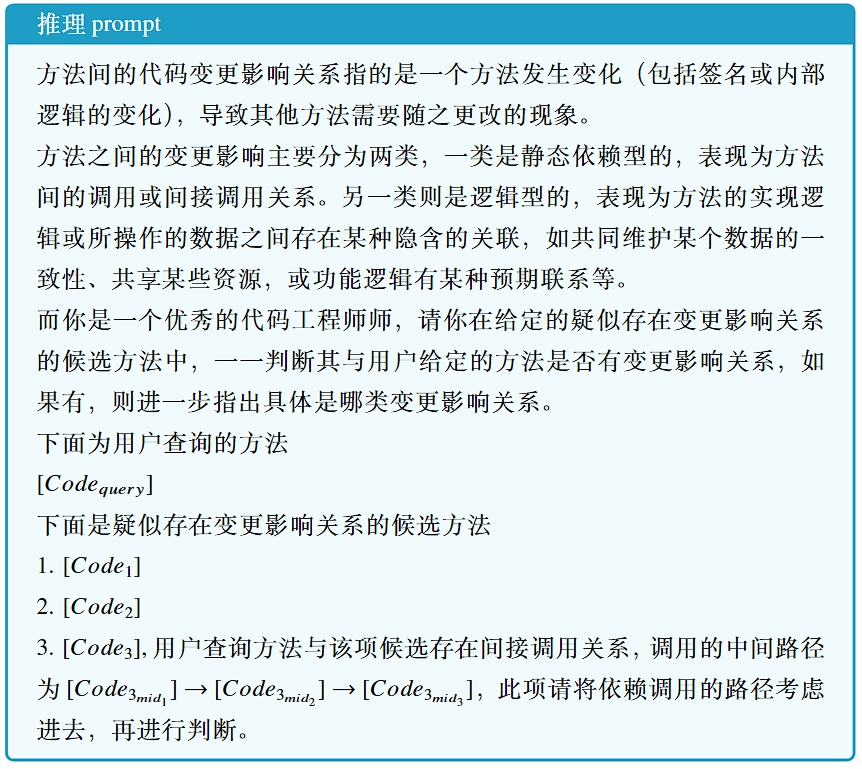
\includegraphics[width = 0.85\textwidth]{figures/2_推理prompt.png}
\caption{生成模块所使用的的Prompt}
\label{2_推理prompt}
\end{figure}


将大语言模型的回复进行解析即可得到与查询方法有变更影响分析的方法。对于有$N$个方法的项目,在实际使用时对于每个查询,需要进行$N$次相似度计算,调用$1$次大模型进行推理,如果上下文长度过长可以对候选方法分片,多次调用大模型,相比于基于代码预训练模型的方法每次需要$N$次的模型前向计算,不仅节省了大量计算时间,还提升了系统的查全率查准率,在实际应用场景中是更好的选择。


\section{实验结果与分析}

\subsection{数据集}
为了便于与前文方法进行性能对比,本章同样选择了六个具有一定规模和影响力的开源代码库作为实验对象,具体包括TheAlgorithms、antiword-0.37、jemalloc-5.3.0、libbpf-1.1、librdkafka-2.1.0和FFmpegKit-5.1.0。这些代码库的选择考虑了其广泛应用和代表性,能够较好地反映方法在实际开发环境中的效果。

鉴于本章提出了一种基于代码依赖的数据清洗方法,嵌入模型所需的训练数据经过重新清洗,以确保其质量和准确性。数据集的收集过程与\ref{1_数据集来源和数据清洗}节中的方法一致。在数据清洗过程中,所使用的模型为Doubao(API模型名:Doubao-lite-32k-240428),该模型在处理代码依赖关系和数据清洗任务方面表现出较高的精度。最终,得到的训练数据的统计信息如表\ref{1_数据集统计信息}所示,共计包含6526对数据。这些数据将用于后续方法的训练。


\begin{table}[htbp]
\caption{训练数据统计信息}
\label{1_数据集统计信息}
\vspace{0.5em}\centering\wuhao
\begin{tabular}{cccc}
\toprule
项目名称 & 三元组数量 \\
\midrule
TheAlgorithms    & 314   \\
antiword-0.37    & 257   \\
jemalloc-5.3.0   & 1023   \\
libbpf-1.1       & 835   \\
librdkafka-2.1.0 & 1524  \\
FFmpegKit-5.1.0  & 336   \\ 
总计              & 4289  \\
\bottomrule
\end{tabular}
\end{table}

\subsection{评价指标} 
评价指标同第\ref{1_评价指标}节,使用Precision,Recall和F-measure来评价模型挖掘变更影响关系的能力。

\subsection{实验设置}

\paragraph{1. 检索模块嵌入模型选择}
MTEB Leaderboard\footnote{https://huggingface.co/spaces/mteb/leaderboard} 是一个实时更新的开源嵌入模型排行榜,专门用于评估不同模型在各种任务中的嵌入能力。为了实现对知识库中代码片段的有效编码,本文从MTEB Leaderboard中选取适合本任务的嵌入模型。选择标准主要包括以下几点:(1)模型在开源嵌入能力评价基准上表现优异,这能够体现其在各类通用文本上的嵌入能力;(2)模型支持的上下文长度大于4k,考虑到代码任务通常涉及较长的上下文,较短的上下文长度可能无法有效捕捉到代码间的复杂关系;(3)模型的参数规模控制在500M以下,综合考虑计算资源和数据规模,超过500M参数规模的模型在使用上的代价较高,难以满足实际应用需求。基于这些选择标准,本文最终选定了如表\ref{2_嵌入模型参数量}所示的5个模型。这些模型在性能、上下文支持以及资源消耗方面都达到了较好的平衡,适合本研究中对代码片段进行嵌入编码的需求。
    
    \begin{table}[htbp]
    \caption{嵌入模型信息}
    \label{2_嵌入模型参数量}
    \vspace{0.5em}\centering\wuhao
    \begin{tabular}{ccc}
    \toprule
    嵌入模型 & 参数量 & 上下文长度  \\
    \midrule
    gte-large-en-v1.5 & 434M & 8192 \\
    jina-embeddings-v3 & 572M & 8192\\
    stella\_en\_400M\_v5 & 435M & 8192 \\
    KaLM-embedding-multilingual-mini-instruct-v1.5 & 494M & 131072 \\
    nomic-embed-text-v1.5 & 137M & 8192 \\
    \bottomrule
    \end{tabular}
    \end{table}
    
\paragraph{2. 嵌入模型训练设置}
在本研究的嵌入模型训练过程中,采用了对比损失函数(InfoNCE Loss)作为目标函数,以确保模型能够有效学习到不同代码片段之间的相似度关系。训练优化器选择了Adam优化器,其中超参数$\beta_1$设置为0.9,$\beta_2$设置为0.95。为提高训练效果,学习率采用余弦衰减策略,使得训练过程中学习率逐渐减小,有助于模型在接近收敛时获得更精细的更新。

Batch size固定为64,以保证每次梯度更新的稳定性。对于较大规模的模型,考虑到内存限制,采用了梯度累计(Gradient Accumulation)技术,通过多次反向传播累积梯度,从而保证了相同的批次大小。学习率初始值设置为1e-4。

在训练阶段,损失函数设置为对比损失函数InfoNCE Loss。训练优化器使用Adam,超参数$\beta_1$设置为0.9,$\beta_2$设置为0.95;学习率采用余弦衰减;Batchsize固定为64,对于规模较大的模型,使用梯度累计方法保证batchsize大小。学习率设置为1e-4。所有实验均在PyTorch框架和Transformer库上实现,确保了高效的模型训练和易于扩展的实现平台。训练过程在单个NVIDIA Tesla V100 32G GPU上进行。
    
\paragraph{3. 生成模型选择}
本章实验中生成模块使用的大模型包含两类:闭源商业模型和开源模型;其中闭源模型包括:GPT4o(API model name:gpt-4o-2024-05-13),Doubao(API model name:Doubao-lite-32k-240428),Kimi(API model name:moonshot-v1-32k);开源模型选择:Qwen2.5-Coder-3B-Instruct ,Llama-3.2-3B-Instruct


\subsection{实验结果与分析}

RQ1:检索模块性能如何,是否能有效地检索到与问询方法存在变更影响关系的方法?

RQ2:本章提出的基于代码依赖与检索增强生成的变更影响关系分析方法性能如何,相比于其他方法表现如何?

RQ3:本章提出的基于代码依赖与检索增强生成的变更影响关系分析方法是否能有效解决间接依赖信息缺失的问题?

RQ4:本章提出的基于代码依赖与检索增强生成的变更影响关系分析方法的跨项目迁移表现如何?
 

\textbf{1.针对于RQ1的实验}

检索模块的嵌入模型表现如表\ref{1_检索模块的召回率与Topk的关系可视化}所示。其中横坐标表示$topk$,即返回检索模块对知识库的相似度排序的前$k$个作为候选,纵坐标表示召回率。虚线为未经训练的嵌入模型,实现表示经过训练的嵌入模型。


\begin{figure}[htbp]
\centering
\includegraphics[width = 1\textwidth]{figures/topk召回率可视化.pdf}
\caption{检索模块的召回率与Topk的关系可视化}
\label{1_检索模块的召回率与Topk的关系可视化}
\end{figure}

可以发现经过训练的模型在本文应用场景性能更好,其中经过训练的stella\_en\_400M\_v5综合表现最佳,考虑到$topk$的大小会对推理速度和召回率产生相反的影响,综合考虑选择$topk=20$作为后续实验的设定。 

\textbf{2.针对于RQ2的实验}

关于生成模块中不同大语言模型对最终性能影响如表\ref{2_不同LLM的实验表现}所示,GPT4o是综合表现最佳的生成模块的选择,即使最小的开源模型Qwen2.5-Coder-3B-Instruct ,Llama-3.2-3B-Instruct也可以超过经过上一章节训练的CodeBERTa模型。

\begin{table}[htbp]
\caption{不同LLM的实验表现}
\label{2_不同LLM的实验表现}
\vspace{0.5em}\centering\wuhao
\begin{tabular}{cccc}
\toprule
方法 & F-measure & recall & precision  \\
\midrule
CodeBERTa & 59.5 & 55.3 & 64.4 \\
Just Retrieval & 32.6 & \textbf{78.1} & 20.6 \\
\midrule
RAG-GPT4o & \textbf{74.8} & 74.6 & \textbf{75.1} \\
RAG-Doubao & 73.4 & 73.8 & 73.1 \\
RAG-Kimi & 71.9 & 71.2 & 72.7 \\
RAG-Qwen2.5 & 65.4 & 63.5 & 67.4 \\
RAG-Llama-3.2 & 64.9 & 62.3 & 67.8 \\
\bottomrule
\end{tabular}
\end{table}


表\ref{2_变更影响实验结果}进一步对于不同类型的影响关系进行分析,可以发现相比于之前方法来讲,基于代码依赖与检索增强生成的方法在两个类型的变更影响关系检测上,均拥有更好的性能。其中依赖型关系的F-measure提升更是达到16.9\%,其中由于增添了检索模块,在两种关系的召回率方面提升显著。

\begin{table}[htbp]
\caption{变更影响实验结果}
\label{2_变更影响实验结果}
\vspace{0.5em}\centering\wuhao
\begin{tabular}{c|ccc|ccc|c}
\toprule
  & \multicolumn{3}{c|}{Dependence-Based} & \multicolumn{3}{c|}{Logic-Based} & Overall \\
\midrule
方法 & F-measure & recall & precision & F-measure & recall & precision  
 & F-measure\\
\midrule
依赖闭包 &  44.8 & 100 & 28.9 & - & - & - & 36.8 \\
克隆检测 &  - & - & - & 31.8 & 19.1 & 95.7 & 3.8\\
共现关系挖掘 &  56.0 & 44.6 & 75.4 & 57.0 & 47.3 & 71.8 & 52.8\\
CodeBERTa  &   61.9 & 56.6 & 68.3 & 71.7 & 73.9 & 69.7 &59.5\\
Just Retrieval   & 34.5 & 82.3 & 21.8 & 36.6 & 88.5 & 23.1 & 32.6\\
RAG & \textbf{78.8} & 78.4 & 79.2 & \textbf{85.4} & 85.9 & 84.9 & \textbf{74.8}\\
\bottomrule
\end{tabular}
\end{table}

\textbf{3.针对于RQ3的实验}

本实验探讨在提示中加入调用路径的中间方法对间接依赖的检测效果的影响。选取测试集中的间接依赖型的变更影响分析子集进行实验,结果如图\ref{2_消融实验}所示。根据结果可以看出在提示中加入调用路径的中间方法对于基于RAG的方法在提升非常显著。

\begin{table}[htbp]
\caption{加入调用路径的中间方法对间接依赖的检测效果的影响}
\label{2_消融实验}
\vspace{0.5em}\centering\wuhao
\begin{tabular}{cccc }
\toprule
  & \multicolumn{3}{c}{Indirect-Dependence-Based}  \\
\midrule
方法 & F-measure & recall & precision \\  
\midrule
CodeBERTa  &  10.7 & 15.1 & 8.3 \\
\midrule
RAG  & 72.6 & 73.5 & 71.7 \\
RAG without 依赖路径  & 14.2 & 12.1 & 17.1 \\
\bottomrule
\end{tabular}
\end{table}


\textbf{4.针对于RQ4的实验}

本实验探讨所提出方法在跨项目的迁移能力,数据集划分同上一章节一样,分为四个分布内代码库和两个分布外代码库。实验结果如表\ref{2_跨项目迁移能力分析}所示。上一章节的基于代码预训练模型的方法,跨项目时性能下降在28.9\% 到 31.7\%之间。本章节的检索模块以及整个RAG系统在跨项目时性能下降仅在 9.2\% 到 11.4\%。


\begin{table}[htbp]
\caption{跨项目迁移能力分析}
\label{2_跨项目迁移能力分析}
\vspace{0.5em}\centering\wuhao
\begin{tabular}{c|cccc|cc}
\toprule
方法& TheAlgorithms & antiword & librdkafka & FFmpegKit & jemalloc & libbpf\\
\midrule
train on 6 datasets:\\
\midrule
CodeBERTa  &  60.23 & 59.64 & 60.18 & 57.87 & 60.99 & 58.22 \\
Just Retrieval   & 32.4 & 32.91 & 31.81 & 36.57 & 33.78 & 35.07  \\
RAG & 76.0 & 78.45 & 76.46 & 77.66 & 79.04 & 76.29  \\
\midrule
train on 4 datasets:\\
\midrule
CodeBERTa  &  62.28 & 65.24 & 63.45 & 62.19 & 41.92$^*$ & 40.8$^*$\\
Just Retrieval   & 33.33 & 34.2 & 34.77 & 36.89 & 29.74$^*$ & 31.09$^*$ \\
RAG & 78.24 & 79.21 & 78.59 & 77.98 & 71.08$^*$ & 69.66$^*$ \\
\bottomrule
\end{tabular}
\end{table}
 

\section{本章小结}

本章提出了基于代码依赖与检索增强生成的代码变更影响分析方法,通过结合依赖路径提升了方法在间接依赖影响上的检测性能,并通过训练检索模块,大幅提升了测试集上的召回率,最后整个系统的综合表现得到了大幅提升。并且通过实验验证了依赖路径加入的有效性。最后在跨项目迁移能力的实验中,基于代码依赖与检索增强生成的代码变更影响分析方法的迁移能力表现优秀,进一步证明了本章所提出的方法的有效性。

%%%%%%%%%%%%%%%%%%%%%%%%%%%%%%%%%%%%%%%%%%%%%%%%%%%%%%%%%%%%%%%%%%%%%%%%%%%%%%%
\chapter{基于代码审查图的代码架构和质量信息可视化}
\section{引言}


在软件开发过程中,开发者通常会经历多个阶段。在项目的初始阶段,开发者需要阅读和理解已有的代码,这是熟悉软件项目的第一步。然而,对于大型项目而言,由于项目代码量庞大,涉及的模块和功能众多,这一过程通常需要耗费大量的时间和精力。除此之外,开发者在对软件进行修改时,如添加新功能或修复缺陷,通常需要深入了解修改代码的上下文信息。如果对上下文理解不清晰,可能会导致变更不完全或不准确,进而影响软件质量。在软件开发的后期,开发者往往需要作为代码审查者参与到代码审查过程中。代码审查的主要目的是评估变更后的代码是否符合质量标准,是否能够顺利地合并到主分支中。这一过程不仅在协作开发中至关重要,也是确保软件质量的有效手段。

然而,代码审查往往需要投入大量的时间和精力\cite{花子涵2024代码审查自动化研究综述}。审查者不仅需要对变更的代码本身进行分析,还需要理解这些代码所处的上下文,才能做出正确的评估。因此,无论是作为开发者还是审查者,理解软件项目的结构和代码是至关重要的。只有深入掌握软件的整体架构和各模块之间的关系,才能在后续的开发和审查过程中保证代码质量。然而,传统的代码阅读和理解方式不仅需要消耗大量的时间和精力,还难以确保高效性和准确性,尤其是在面对庞大复杂的代码库时。

为了提高代码理解的效率并减少人为错误,本文提出了一种基于代码审查图的代码质量分析展示方式。这一方法通过将项目中的各个方法和全局变量表示为图的节点,并用边表示方法与方法之间、方法与全局变量之间的依赖关系,从而形成一个结构化的代码关系图。这样的图形化展示方式能够帮助开发者和审查者从宏观的角度掌握整个软件项目的架构和各个模块之间的关系,进而提升对代码的理解效率。通过这种方式,开发者和审查者可以更直观地识别出项目中的关键部分及其相互依赖关系,从而在变更和审查过程中更高效地评估代码的质量和影响。


\section{基于代码中间表示的代码质量度量提取}

代码内聚度和代码耦合性是衡量软件设计质量的两个核心指标,它们直接反映了代
码模块化质量。代码内聚度指的是模块(如文件、类或组件)内部元素之间的相关性。高内聚度意味着模块内的所有元素都紧密地围绕着一个单一的、明确的功能,代码更容易理解和维护\cite{2014Service}。代码的耦合性则描述了模块之间的相互依赖。低耦合度意味着模块之间的依赖关系较小,每个模块都可以独立地执行其功能,而不需要过多地依赖其他模块。低耦合度的代码更容易测试和维护\cite{2013Ahe}。除此之外我们还考虑了代码的复杂性和代码缺陷,对


基于方法摘要和全局变量信息表,我们计算如下代码度量,用于分析代码质量。


\subsection{基于内聚度缺乏度的内聚性分析}

LCOM(Lack of Cohesion in Methods)系列指标是根据模块内聚度的缺乏程度来衡量模块的内聚度的指标。在本文中,
面向对象语言以类为研究范围进行计算内聚度,非面向对象的语言以文件为研究范围进行计算,类中的成员属性对应文件中的全局变量,类中的成员方法对应文件中定义的方法。LCOM 指标的核心思想是度量一个类中方法对实例变量(属性)的共享程度。不同版本的 LCOM 有着不同的计算方法和含义,体现了不同的侧重点。这里一共计算以下四个指标,

(1)LCOM1,含义是不引用相同字段的方法对数目\cite{1994Ametr}。计算公式如式(2-1)。
\begin{equation}
LCOM1 = C_{n}^{2}-e
\end{equation}

其中n 是文件中的方法总数,e 是引用相同字段的方法对。以图2-4为例介绍计算方式,其中椭圆表示方法,点表示变量,点在椭圆内表示该方法引用了该变量。LCOM1值为\(C_{6}^{2} - 5 = 10\)。

\begin{figure}[h]
\centering
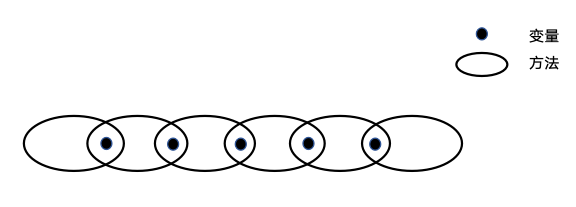
\includegraphics[width = 0.7\textwidth]{内聚度示例.jpg}
\caption{示例模块}
\end{figure}
    

(2)LCOM2,含义是不引用相同字段方法对与引用相同字段方法对数之差\cite{1996Coupling}。其计算公式如式(2-2)。

\begin{equation}
    {LCOM2}=\left\{
        \begin{array}
        {c}P-Q,  ifP\geq Q \\
        0,  otherwise
        \end{array}\right.
\end{equation}

其中,P 是不共享实例变量的方法对的数量,Q 是共享实例变量的方法对的数量。
如果 LCOM1 的结果为负数,则被置为 0。图2-4模块中,不共享变量的方法对P为10,共享变量的方法对Q为5,LCOM2值为P-Q=5。

(3)LCOM3是对前两种指标的进一步改进,其计算公式如式(2-3):
\begin{equation}
LCOM3 = \frac{\left( \frac{1}{a} \sum_{j=1}^a \mu(A_j) \right) - m}{1 - m}
\end{equation}

其中\( m\)为文件中的方法数,\( a\)表示文件中的变量数,\( mu(A_j)\)表示的是引用变量\(A_j\)的方法数。如图2-5所示的文件中有3个方法和3个变量,计算方式如图所示。
\begin{figure}[h]
\centering
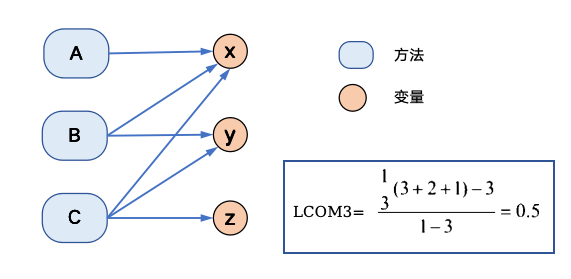
\includegraphics[width = 0.7\textwidth]{LCOM3.jpg}
\caption{LCOM3计算示例}
\end{figure}



(4)LCOM4,含义是以方法和变量为顶点,方法引用字段或方法之间有调用关系则两节点之间有条边构成图的连通分支数\cite{1995Measuring}。计算时,根据深度优先搜索的方式,计算图中的连通分支数,得到的值即为LCOM4。如图2-6所示的两个文件的LCOM4的值分别为2和1。

\begin{figure}[h]
\centering
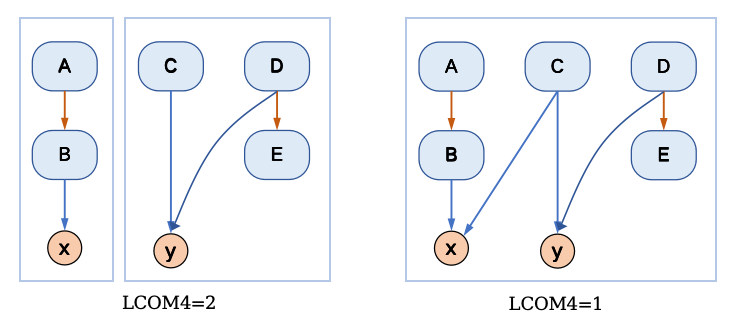
\includegraphics[width = 0.7\textwidth]{LCOM4.jpg}
\caption{LCOM4计算示例}
\end{figure}

\subsection{基于连通性的内聚性分析}
TCC(Tight Class Cohesion)和 LCC(Loose Class Cohesion)是用于衡量模块内
聚度的指标,这两个指标主要关注于模块中方法之间的连通关系,核心思想是通过
分析模块中方法如何相互作用以及如何访问共同资源(如全局变量)来评估模块的内聚度。


(1)TCC,含义是有连通关系的方法对数与总方法对数的比值\cite{1995Cohesion}。
TCC 关注于模块中方法之间的“直接连接”。如果两个方法直接共享访问同一个变
量,则认为这两个方法是直接连接的。计算公式如式(2-4)。
\begin{equation}
{TCC} = \frac{e}{C_{n}^{2}}
\end{equation}

其中\(n\)是文件中的方法总数,\(e\)是图中的直接连接边数。

(2)LCC则基于方法间接引用共同字段的关系进行计算\cite{1995Cohesion}。
LCC 除了考虑直接连接的方法对外,还包括了间接连接的方法对。如果两个方法不
是直接连接,但可以通过一系列的方法调用或变量引用来连接,则认为它们是间接连接的。LCC 的值基于模块中直接或间接连接的方法对占所有可能方法对的比例来计算。因此,LCC 的值通常不低于 TCC 的值,并且提供了一个更宽泛的模块内聚度视角。计算公式如式 (2-5):
\begin{equation}
{LCC=\frac{e+e_{indirect}}{C_{n}^{2}}}
\end{equation}

其中\(n\)是文件中的方法总数,\(e\)是图中的直接连接边,\(e_{indirect}\)是除直接连接边的边数。如图2-7是计算LCC和TCC的例子,左图中通过方法AB通过变量x直接连接,方法CD通过变量y直接连接,直接连接和间接连接都是2。而右图中直接连接是AB、BC、BC和CD,间接连接是AD和BD,因此计算结果如图。

\begin{figure}[h]
\centering
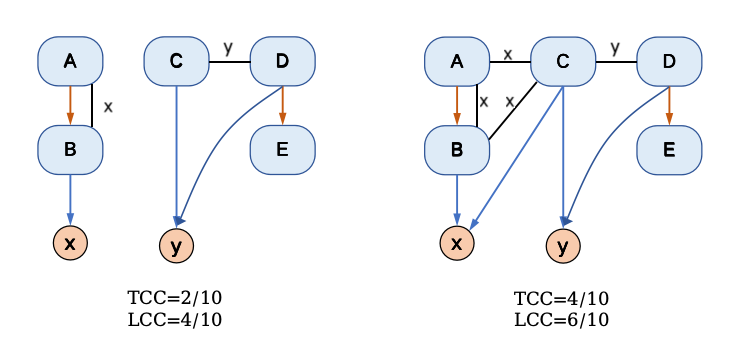
\includegraphics[width = 0.7\textwidth]{TCCLCC.jpg}
\caption{TCC和LCC计算示例}
\end{figure}


\subsection{方法间耦合性分析}

耦合是在软件架构中用来描述模块间相互依赖和连接程度的一个重要指标。耦合度的高低直接影响到系统的维护性和可扩展性。在现有的研究和实践中,耦合度通常被细分为六个等级,如表2-1所示,这些等级从高到低反映了模块间依赖的紧密程度。本文关注的是方法与方法之间的耦合性,方法间的耦合性反映了不同方法之间的依赖关系,它直接影响代码的可读性、可测试性以及后续的维护和扩展。通过深入分析方法级别的耦合性,研究方法如何通过参数传递、调用关系、共享全局变量等方式相互依赖,我们可以更准确地识别潜在的设计缺陷和优化机会,从而提高系统的模块化程度,增强系统的可维护性和可扩展性。

\begin{table}[htbp]
\caption{软件架构中耦合性分类}
\vspace{0.5em}\centering\wuhao
\begin{tabular}{ccccc}
\toprule
耦合性类别 & 描述 & 耦合程度 & 本文是否分析 \\
\midrule
内容耦合 & 模块直接访问或修改另一个模块的内部数据 & 6 & 否\\
公共耦合 & 模块访问同一公共数据环境 & 6 & 是 \\
外部耦合 & 模块共享全局简单数据结构 & 4 & 是 \\
控制耦合 & 模块传递控制信息,影响计算流程 & 3 & 否 \\
标记耦合 & 通过参数传递复杂数据结构信息 & 2 & 是 \\
数据耦合 & 通过参数传递简单数据 & 1 & 是 \\
\bottomrule
\end{tabular}
\end{table}


内容耦合是耦合度最高的一种形式,它表示一个模块能够直接访问或修改另一个模块的内部数据和结构。在方法级的耦合分析中,这种耦合形式通常不被考虑,因为方法间的直接数据访问往往通过参数传递或者 API 调用实现,而不是直接的内容访问。

公共耦合发生在多个模块共同访问某个全局数据环境时。这种数据环境可能是全局数据结构、全局变量或内存公共区域等。在提取到的全局变量表中,对于复杂数据结构如结构体和数组,其引用点所在的方法之间均存在公共耦合关系。


外部耦合与公共耦合相似,但区别在于它涉及的是对全局简单变量的访问。例如,当多个模块访问或修改相同的全局简单类型变量时,则这些模块之间存在外部耦合。


控制耦合指模块之间传递信息中包含用于控制模块内部的信息。在提取到的方法摘
要表中,遍历方法,如果该方法调用其他方法时,对应方法的参数列表中有变量决定了被调用方法中的计算流程,则方法之间存在控制耦合关系。由于本文不考虑分析方法内部的控制逻辑,因此不提取此种耦合。


标记耦合指通过参数表传递数据结构信息,调用时传递的是数据结构。在方法摘要
表中提取了方法的参数列表,包括参数名和参数类型,根据参数类型,可以确定
参数表中是否包含复杂类型。除此之外,在方法的调用表中,也提取了方法调用的
其他方法,结合这两个信息,即可确定两个方法是否存在着标记耦合关系。


数据耦合指通过参数表传递简单数据。与标记耦合类似,根据参数类型可以确定参
数是否全部为基本类型,结合方法调用表,即可确定两个方法是否存在数据耦合。
\subsection{方法扇入扇出度量分析}

方法的扇入(Fan-in)和扇出(Fan-out)是软件工程中用于衡量方法复杂性和模块
间依赖关系的两个指标。

\begin{figure}[h]
\centering
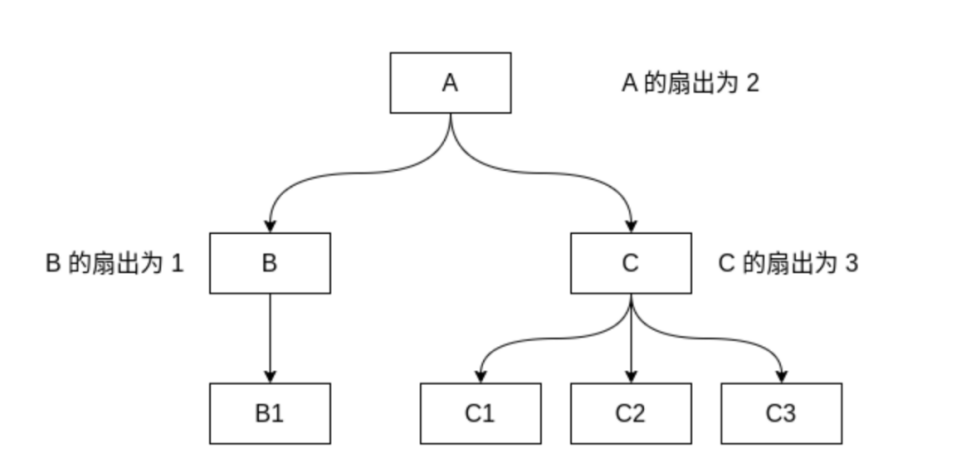
\includegraphics[width = 0.8\textwidth]{扇入扇出.png}
\caption{扇入扇出实例}
\end{figure}
    

扇入是指调用某个方法的不同方法的数量。它表示了一个方法对其他方法的依赖程
度。扇入值较高的方法通常被认为是重要的或核心的,因为它们被多个其他方法所依赖。
高扇入值可能意味着该方法执行了一个基础或共享的任务。


扇出是指某个方法直接调用的不同方法的数量。它表示了一个方法对其他方法的影
响程度。扇出值较高的方法可能更复杂,因为它们需要管理和协调更多的方法调用。高
扇出值可能意味着该方法具有较高的责任度,且可能更难以理解和维护。


本文中对于提取到的方法摘要表,遍历每一个方法,统计其调用方法的数量即可计算出该
方法的扇出值,再以该方法名在方法摘要表中搜索调用了该方法的方法,统计总数,得
到的值即为扇入值。

\subsection{基于静态检测工具的代码缺陷检测}

为了更准确地衡量代码质量,本文结合了静态代码分析工具 Cppcheck,对项目中的源代码进行检测和分析。Cppcheck 是一款开源的静态分析工具,专门用于检测 C/C++ 代码中的潜在错误和编码规范问题。它通过静态分析技术,扫描源代码,识别可能存在的内存泄漏、空指针解引用、未初始化变量等常见问题,并提供详细的诊断报告。与传统的编译器警告不同,Cppcheck 不依赖于程序的编译过程,它直接分析源代码的结构和逻辑,从而能够发现更广泛的潜在问题,尤其是那些难以通过常规测试手段捕捉到的错误。

在本研究中,Cppcheck 的检测结果被视为代码质量评估的重要组成部分。Cppcheck会根据问题的严重性和类别将检测出的问题如表2-2所示的六类。

\begin{table}[htbp]
\caption{cppcheck报告问题分类}
\vspace{0.5em}\centering\wuhao
\begin{tabular}{cccc}
\toprule
类别 & 描述 \\
\midrule
error &  严重错误 \\
warning & 潜在的错误或不推荐的做法 \\
style & 代码风格问题,通常与代码格式、命名约定等相关 \\
performance & 性能问题,表明当前方式可能效率不高 \\ 
portability & 平台相关问题,可能导致在不同环境出现不同行为 \\
information & 额外的信息或建议 \\ 
\bottomrule
\end{tabular}
\end{table}

检测结果中包括了诸如错误、警告和代码风格问题等不同级别的信息,这些信息帮助开发者识别代码中的潜在问题并及时修复,进而提高代码的可维护性和健壮性。

Cppcheck 提供的报告与其他度量指标相结合,共同构成了全面的质量评估体系。用户可以根据检测报告对代码质量进行更细致的判断和分析,从而为后续的优化和重构提供科学依据。通过这种方式,本研究实现了对代码质量的多维度综合评价,为开发者提供了更为精确的质量检测和改进方向。

\section{代码审查图}

\subsection{代码审查图构建}

代码审查图主要由两个核心元素构成,即节点和边。其中,节点代表软件项目中的方法或全局变量,边则表示节点之间的各种关系,如耦合关系、变更影响关系以及依赖调用关系。这些元素的结合能够帮助开发者从全局视角理解和评估项目的结构和质量,尤其是在进行代码审查和变更分析时。

(1)节点属性

在代码审查图中,节点的作用是标识项目中的方法和全局变量。通过前文所述的方法摘要表和全局变量信息表,我们为每个方法和全局变量创建了对应的节点。每个节点都具有多个属性,这些属性能够提供有关节点所代表的方法或变量的关键信息,便于开发者对代码进行全面的审查和分析。

方法属性分为两个主要部分:,首先是方法的基本信息,如表4-1所示。

\begin{table}[htbp]
\caption{代码审查图节点属性-基本信息}
\vspace{0.5em}\centering\wuhao
\begin{tabular}{cccc}
\toprule
    属性 & 描述 \\
\midrule
方法名 & 方法名,由方法所在路径和方法名拼接而成,保证唯一  \\
方法参数 & 方法的参数列表,包括参数的名称和类型   \\
方法内调用方法 & 本方法内调用的其他方法名   \\
方法可作用域 & 表明方法是否全局可用   \\
方法所在模块 &  方法所在模块,目前表示为方法所在文件  \\
模型预测方法模块 & 模型预测的方法应在的模块   \\     
\bottomrule
\end{tabular}
\end{table}

这一部分包括方法的名称、所在模块、方法签名、访问修饰符等基本信息,这些信息有助于开发者快速识别和定位方法的功能和作用。例如,方法的名称可以反映其业务功能,所在模块和调用信息则有助于理解方法的上下文和调用约束。

其次是与代码质量相关的度量和信息,如表4-2所示。

\begin{table}[htbp]
    \caption{代码审查图节点属性-质量相关信息}
    \vspace{0.5em}\centering\wuhao
    \begin{tabular}{ccp{9cm}}
    \toprule
    属性类别 & 属性 & 描述 \\
    \midrule
    \multirow{2}{*}{扇入扇出信息}& 扇入 &  方法的扇入值以及扇入值在项目中的排名比例 \\       
                                & 扇出 &  方法的扇出值以及扇出值在项目中的排名比例 \\   \cline{2-3}
    \multirow{2}{*}{内聚度信息}& LCOM1 &  所在模块的LCOM1值以及相应建议 \\       
                                & LCOM2 &  所在模块的LCOM2值以及相应建议 \\    
                                & LCOM3 &  所在模块的LCOM3值以及相应建议 \\    
                                & LCOM4 &  所在模块的LCOM4值以及相应建议 \\    
                                & TCC &  所在模块的TCC值以及相应建议 \\    
                                & LCC &  所在模块的LCC值以及相应建议 \\   \cline{2-3}             
    \multirow{2}{*}{耦合关系}& 数据耦合 &  与本方法存在数据耦合关系的方法 \\       
                                & 标记耦合 &  与本方法存在标记耦合关系的方法 \\   
                                & 外部耦合 &  与本方法存在外部耦合关系的方法 \\   
                                & 公共耦合 &  与本方法存在公共耦合关系的方法 \\   \cline{2-3}
    变更影响关系 & 变更影响关系 &  与本方法存在变更影响的方法,表明来源为代码克隆、变更历史、模型预测 \\    \cline{2-3}
    缺陷 & 静态代码缺陷 &  由cppcheck检测得到的本方法缺陷 \\      
    \bottomrule
    \end{tabular}
    \end{table}

这一部分基于前文方法提取和统计结果,涵盖了一些与代码质量直接相关的指标,如方法的扇入扇出、内聚度、耦合性等。这些度量和指标的结果将结合项目的具体统计数据或检测结果,向开发者提供有针对性的改进建议。例如,如果某个方法的扇出度位居项目中的前5\%,则可能表明该方法在项目中的依赖关系过于复杂,可能导致高耦合性,进而影响系统的灵活性和可维护性。类似地,如果检测出某方法存在不良耦合,则可能需要开发者重新设计该方法与其他模块的接口,以减少不必要的依赖。



对于全局变量的属性则主要包含表4-3中的信息。主要是对全局变量基本信息的展示,方便开发者快速了解该变量的作用域、使用情况以及与其他代码部分的关联性。通过这些信息,开发者能够更好地理解变量在整个项目中的作用及其潜在的质量风险。

\begin{table}[htbp]
\caption{代码审查图节点属性-全局变量信息}
\vspace{0.5em}\centering\wuhao
\begin{tabular}{cccc}
\toprule
    属性 & 描述 \\
\midrule
变量名 & 全局变量名,由所在路径和变量名拼接而成,保证唯一  \\
变量类型 & 变量类型   \\
被使用方法 & 使用了本全局变量的方法名   \\
变量可使用域 & 表明变量是否全局可用   \\
方法所在模块 &  变量所在模块,目前表示为所在文件  \\  
\bottomrule
\end{tabular}
\end{table}


(2)边的设计

在代码审查图中,边表示节点与节点之间的关系,这些关系揭示了软件系统中各个方法与全局变量之间的相互依赖和影响。根据其性质,边的类型主要分为三类,具体分类如表4-4所示:静态依赖关系、耦合关系和变更影响关系。

其中静态依赖关系分为方法之间的调用关系和方法与全局变量的引用,耦合关系如表4-2中所示共4类,变更影响关系则根据检测方法的不同,设定为3个不同的来源。需要注意的是,由于依赖闭包方法本身是基于依赖图生成的,因此在代码审查图中,这类关系不再单独指出。

每种关系反映了不同层次的代码相互作用,帮助开发者全面理解系统的结构和潜在的质量风险。

\begin{table}[htbp]
\caption{代码审查图边分类}
\vspace{0.5em}\centering\wuhao
\begin{tabular}{cccc}
\toprule
属性 & 描述 \\
\midrule
静态依赖关系 & 含方法之间调用、方法引用全局变量两种  \\
耦合关系 & 含数据耦合,标记耦合,外部耦合,公共耦合四种   \\
变更影响关系 & 含代码克隆、变更历史、模型预测三种  \\
\bottomrule
\end{tabular}
\end{table}



\subsection{代码审查图可视化}

本节从代码审查图的可视化方案和交互方案两个方面展开介绍。

1.可视化方案 

代码审查图的可视化方案基于开源项目 G6。G6 是一个强大的图形可视化引擎,提供了绘制、布局、分析、交互、动画等全方位的图形可视化基础功能,具有简单易用且完备的特性。G6 具有两个显著优势。

(1)数据与可视化图形分离:在使用 G6 时,用户只需将图的数据组织为 JSON 格式,如图4-3所示,包括节点信息和边信息,直接传递给 G6 即可自动生成对应的力导向图。这种数据与图形的分离不仅简化了开发流程,还提高了数据的灵活性和可操作性,便于进行后续的数据更新和图形重绘。

\begin{figure}[h]
\centering
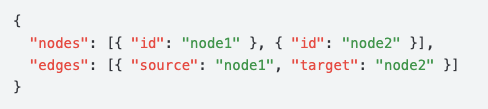
\includegraphics[width = 0.6\textwidth]{G6图数据示例.jpg}
\caption{G6图数据示例}
\end{figure}

(2)高度的定制能力:G6 提供了丰富的图形展示配置选项,用户可以根据需求自由选择不同的样式和布局方式。如果 G6 内置的元素不满足特定需求,它还支持用户自定义节点、边及其他元素,使得图形展示更加贴合实际应用场景。

本文使用G6内置节点和边实现代码审查图的可视化。G6的节点构成共包含6部分,其中label表示文本标签,通常用于展示节点的名称或描述,本文中将节点属性赋值给label,便于用户查看属性相关信息。G6的边的构成共包含4部分,label具有同样的功能,将边的类别用于label。让 G6 加载此数据源进行展示,就实现了同时也实现了计算逻辑与图形可视化的有效分离。


2.交互方案

对于软件项目这样的分析对象,方法和全局变量的数量常达到千级别,这样的级别对于一个图来讲,很难在图中展示完所有的信息,因此需要用户交互,来展示更详细的信息。表4-5展示了目前代码审查图的交互和对应的逻辑设计。


\begin{table}[htbp]
\caption{代码审查图交互和逻辑设计}
\vspace{0.5em}\centering\wuhao
\begin{tabular}{cccc}
\toprule
交互方式 & 业务逻辑 \\
\midrule
视角缩放 & 操作鼠标滚轮对图进行缩放  \\
视角移动 & 鼠标拖拽移动整个代码审查图   \\
聚焦节点 & 光标悬停在节点上显示节点的方法名/变量名  \\
移动节点 & 鼠标长按节点拖拽可移动节点 \\
查看节点属性 & 鼠标点击节点展开节点属性  \\
聚焦关系 & 光标悬停在边上显示边的类型  \\
查看关系信息 & 鼠标点击节点展开节点属性  \\
节点筛选 & 通过点击筛选节点按钮,确认是否筛选掉孤立节点 \\
\bottomrule
\end{tabular}
\end{table}



\subsection{代码审查报告生成}

在软件开发和代码审查的过程中,开发者通常可以借助代码审查图聚焦于代码的上下文,帮助发现局部代码的问题。然而,当软件开发完成,开发者希望从全局角度对软件项目的整体质量进行衡量时,仅依靠代码审查图可能会存在质量信息过于分散、不易聚焦的问题。因此,本研究进一步提出通过生成文档化的代码审查报告,为开发者提供统一的代码质量概览,帮助其全面掌握项目的质量状况。

代码审查报告的核心目标是揭示软件项目中存在的关键质量问题,并以本文提取的代码质量属性为主线,系统性地向用户报告代码中的潜在问题。具体来说,报告主要涵盖以下几个方面的内容:

\begin{itemize}
    \item 内聚度信息:报告中将重点标记内聚度最差的 5\% 模块,并提供相应的统计信息。这些模块通常在逻辑结构上松散、职责分散,可能是代码设计需要改进的关键部分。开发者可通过这些信息快速识别项目中存在高维护风险的模块。
    
    \item 不良的耦合信息:包括同模块内的公共耦合、不同模块的公共耦合以及外部耦合。这些耦合关系可能导致模块之间的高依赖性和低灵活性,影响系统可维护性。
    
    \item 复杂度信息:报告将筛选出扇入扇出指标最差的 5\% 模块,提供详细数据说明。这些模块往往由于过多的依赖关系或调用关系而难以维护,是优化的重点对象。
    
    \item 代码缺陷与规范信息:cppcheck 检测出的代码缺陷和不符合规范的代码信息,并给出相应的建议。
    
    \item 不良变更影响:通过分析代码中的变更影响关系,报告将重点指出项目中存在变更影响关系数量最多的前 5\% 方法。这些方法通常具有较高的变更复杂度,是项目维护中的风险点。
    
    \item 基于大模型的模块预测结果:报告列出那些标签不属于原始模块的方法名称。此类方法可能存在职责划分不当或模块归属不合理的情况,报告将此信息提供给用户,供其判断是否需要重新划分模块归属,从而优化模块结构。
\end{itemize}

为了帮助用户在代码开发过程中防止变更不完全,报告还将列出项目中所有的代码变更影响关系。用户可以参考这些信息,在变更时全面评估影响范围,降低遗漏风险。

通过对这些信息的整合与分析,生成的报告文档为用户提供了一份全面的代码质量概览,既可以帮助用户识别代码中的潜在问题,又能为系统的后续优化与维护提供指导性建议。

\section{实验结果与分析}

\subsection{实验环境与评价方法}

本章依旧使用第二章中的项目为示例项目。

(1)实验环境

实验环境如表4-6所示。

\begin{table}[htbp]
\caption{实验环境}
\vspace{0.5em}\centering\wuhao
\begin{tabular}{cccc}
\toprule
    环境 & 信息 \\
\midrule
操作系统 & macOS Ventura v13.5.2  \\
Intellij pycharm & 2021.1.1   \\
python & 3.7   \\
Java & 1.8   \\
G6 & g6.min.js 4.3.11  \\  
libclang & 15.0.7  \\ 
pycparser & 2.21  \\
\bottomrule
\end{tabular}
\end{table}



(2)评价方法


对于代码审查图生成方法,首先对示例项目生成代码审查图,验证可视化方案的需求,根据代码审查图分析前文中实验结果中的实例研究,以说明代码审查图相较文字的优越之处。

对于代码审查报告的生成,则是验证审查报告的格式是否符合设计方案。

\subsection{实验结果分析}


将实验项目的github仓库克隆到本地,对每个项目进行按前文所述步骤提取代码中间表示,包括抽象语法树、方法摘要表和全局变量信息表,再进一步按2.5节所述方法,提取代码质量度量和缺陷信息。在提取到质量度量后,筛选质量较差的代码分析结果报告给用户,收集用户的反馈,衡量方法的有效性。报告的标准如下:

(1)内聚度

内聚度是衡量一个模块内部各个组件(本文中是方法和全局变量)之间关系的紧密程度的指标。内聚度越高,则意味着模块内的各个部分越紧密,职责明确且功能聚焦。然而,仅凭数值的计算,用户可能难以直观理解模块的内聚度高低。因此本文通过对同一项目中各模块内聚度进行排名,向用户报告内聚度最差的前5\%模块,以帮助用户识别和定位项目中内聚度较差的模块。随着用户不断进行改进,模块的内聚度将逐步提升并收敛,最终整个项目达到平衡的状态。

(2)耦合性

本文中提取了四种不同的耦合类别,每种类别的耦合程度并不相同,数据耦合、标记耦合、外部耦合、公共耦合,耦合程度依次递增。\inlinecite{迟曲2011关于软件设计的模块独立性分析}中提到数据耦合是最佳的耦合类型,而外部耦合和公共耦合则对系统的质量和维护性有负面影响。这是由于数据耦合和标记耦合都通过参数传递数据,方法的输入输出明确,易于测试和维护,而外部耦合和公共耦合共享公共数据,可能会影响程序的可测试性和问题的排查诊断。

本文进一步将代码是否处于同一模块考虑在内,因为对于同一模块内,代码往往有共同的上下文和职责范围,因此可适当对耦合标准放宽。因此对与在同一模块内的方法,报告公共耦合,对于不在同一模块内的方法,报告外部耦合和公共耦合,将这两种情况作为不良耦合报告给用户。

(3)扇入扇出

传统标准中要求尽量高扇入低扇出,高扇入表示其他模块依赖该模块,模块的功能可能是系统中其他模块的核心或基础,复用性较好;低扇出表示该模块没有过多地依赖其他模块,因此它具有更高的独立性,更易维护。同内聚度类似,仅计算数值或统一设置阈值的方式,用户难以直观理解,因此这里也对同一项目中扇入扇出值进行排序,向用户报告最差的前5\%的方法。

(4)静态分析工具

本文结合了静态分析工具Cppcheck对项目代码进行检测。考虑到Cppcheck的严重等级分类能从错误、警告、风格、性能、未定义行为等多个角度提供细致分析,每个类别都关注特定的代码问题,不仅帮助开发者准确识别出可能导致崩溃或异常行为的缺陷,还能够进行规范检查,发现影响程序效率、可读性、资源管理等方面的潜在问题。因此本文将向用户报告表2-2中六种类型的问题,作为质量评估的一部分,提供给用户进行判别。

总的来讲,这四种度量向用户报告的标准如表2-4所示。

\begin{table}[htbp]
\caption{各度量报告标准}
\vspace{0.5em}\centering\wuhao
\begin{tabular}{cccc}
\toprule
度量 & 报告标准 \\
\midrule
内聚度 &  6项指标分别报告内聚度最差的前5\%模块 \\
\multirow{2}{*}{耦合性} &  同模块内报告公共耦合\\
                        & 不同模块报告公共耦合、外部耦合 \\
扇入扇出 & 分别报告最差的前5\%方法 \\
静态工具检测 &  报告6种类型问题\\ 
\bottomrule
\end{tabular}
\end{table}

为了验证质量度量的可靠性与实用性,本文邀请了四位经验丰富的软件开发者,对报告的每一项的准确性和可接受性进行评估。评估的标准包括以下几个方面:

\begin{itemize}
    \item 内聚度差、耦合不良、扇入过低、扇出过高和缺陷的检测结果是否能为用户所接受:评估这些指标的报告内容是否准确反映了代码中的问题,且是否能够为开发者提供有效的指导。
    \item 指标的解释与建议是否有助于代码优化:不仅是检测结果本身,还需要评估报告中对检测结果的解释是否充分。
    \item 报告结果与实际代码质量的关联性:通过比较报告中的分析结果与开发者实际编码过程中所遇到的问题,验证报告的实用性。
\end{itemize}

对于报告的每一项,如果用户认为符合标准,则认为用户接受对应的结果,则将对应的项反馈结果标记为1,统计用户的接受率,接受率指标计算公式如式(2-6)
\begin{equation}
    AR_n =  \frac{\frac{1}{N} \sum_{i=1}^{N} A_i}{T} \times 100\%
    \end{equation}
其中AR表示接受率,A表示开发者接受的项数,T表示报告的总项数,N表示软件开发者数。

1. 内聚度实验结果及实例分析

(1)内聚度实验结果

表2-5展示了对于内聚度报告项用户的接受率,从实验结果可以看出,该方法表现良好,可靠性较高。具体来讲,指标基本都在70\%以上。通过进一步对比,发现在TheAlgorithms、antiword等比较简单的项目中,内聚度在6项指标中常出现相同的接受率,经过分析发现这是因为在同一项目中,尽管6项指标的计算方式和侧重点都不同,但是最差的前5\%基本上是重合的,这意味着一个模块如果在LCOM1中表现的很差,在其他指标中也通常表现得很差,这符合通常认知,同时也侧面验证了指标的准确性。但是对于FFmpegKit等较复杂的项目,6项指标则不太相同,体现了不同内聚度计算方式的侧重点。

\begin{table}[htbp]
\caption{内聚度接受率}
\vspace{0.5em}\centering\wuhao
\begin{tabular}{ccccccc}
\toprule
项目名称 & LCOM1 & LCOM2 & LCOM3 & LCOM4 & TCC & LCC \\
\midrule
TheAlgorithms & 89.2 & 74.9 & 74.9 & 89.2 & 74.9 & 74.9 \\
antiword-0.37  & 91.3 & 84.2 & 84.2 & 91.3 & 84.2 & 84.2 \\
jemalloc-5.3.0 & 82.2 & 82.2 & 82.2 & 82.2 & 88.6 & 88.6 \\
libbpf-1.1 & 87.3 & 83.4 & 87.3 & 87.3 & 93.7 &  93.7 \\
librdkafka-2.1.0 & 73.7 & 73.7 & 73.7 & 73.7 & 78.4 & 78.4 \\
FFmpegKit-5.1.0 & 71.3 & 69.2 & 74.9 & 76.6 & 89.3 & 84.9 \\

\bottomrule
\end{tabular}
\end{table}


(2) 内聚度实例分析

对内聚度实验结果进行进一步分析,这里选取 antiword 项目中的内聚度表现最差的模块 misc.c 文件模块进行分析。为了更好地理解这一现象,进一步检查了该模块的源代码,并对其结构进行了统计分析。具体来看,misc.c 文件中一共定义了 1 个全局变量和 15 个方法,其中 11 个方法并未被同一模块内的其他方法调用,只有 3 个方法之间存在相互调用关系,而仅有 2 个方法使用了该模块定义的全局变量。

通过这个结果可以发现,尽管该模块包含了一定数量的方法和变量,但模块内各个方法和变量之间的依赖关系极为薄弱。大部分方法相互之间没有调用关系,且仅有少数方法与全局变量发生交互。这样的结构表明,模块内的功能划分较为松散,各个功能单元之间缺乏必要的协作和紧密联系。因此,该模块的内聚度较差,功能的集中性和一致性较低,导致其内聚度值显著较低。因此,通过对 misc.c 文件内聚度的分析,我们不仅可以得出该模块的内聚度较差的结论,还能为未来的重构和优化提供指导意见。例如,增强模块内部方法之间的调用关系,优化变量的使用方式,以提高模块的内聚度,从而提升系统的整体质量和可维护性。

2. 其他度量实验结果及实例分析

表2-6展示了对于其他度量报告项用户的接受率,从实验结果可以看出,不同项目在各项度量指标上的接受率存在一定差异。大部分项目的耦合性接受率较高,而扇入扇出的接受率普遍较低,大部分的项目上只达到了40-50\%的水平,而所有项目对静态工具检测出来的缺陷上的接受率都较高,说明静态工具的可靠性较好。接下来对所有指标的实验结果进行进一步分析。

\begin{table}[htbp]
\caption{其他度量接受率实验结果}
\vspace{0.5em}\centering\wuhao
\begin{tabular}{cccc}
\toprule
项目名称 & 耦合性接受率 & 扇入扇出接受率 & 静态工具缺陷接受率 \\
\midrule
TheAlgorithms & 99.2 & 87.6 & 100.0 \\
antiword-0.37 & 84.2 & 56.4 & 98.0 \\
jemalloc-5.3.0 & 77.8 & 66.3 & 100.0 \\
libbpf-1.1 & 68.3 & 42.1 & 100.0 \\
librdkafka-2.1.0 & 63.7 & 48.7 & 98.8 \\
FFmpegKit-5.1.0 & 54.0 & 43.3 & 94.6 \\
\bottomrule
\end{tabular}
\end{table}

(1)耦合性结果分析和实例分析

耦合性的接受率在几个项目中的表现不尽相同。对于结构较为简单的项目,如antiword和jemalloc,接受率均能达到较高的水平,在TheAlgorithms项目上甚至能达到99\%以上的接受率。而对于更大型更复杂的项目,接受率则略微降低。

进一步分析如此表现的原因,对于TheAlgorithms,这个项目是对各种算法的开源实现,模块和模块之间几乎不存在相互依赖和调用的情况,每种算法独立开发,实际上是库函数,仅在需要时供开发者调用。总的来讲,简单项目结构较为简单,各个模块功能明确,职责聚焦,所以耦合性不良的样例很少,共检测出15例。维护起来也更加容易,用户更容易接受。

而在复杂项目中,如FFmpegKit,耦合性接受率相较其他项目低一些。这里以FFmpegKit项目中不被用户所接受的样例进行分析。在这个样例中,方法probe\_file与另外三个模块的方法发生了公共耦合,具体来讲这几个方法共同使用了fftools\_ffprobe.c文件中定义的全局变量nb\_streams,这是一个整数。而不被用户所接受的理由是,这个全局变量实际上是一个共享全局状态,它代表了流的数量,需要在不同平台上保持一致,如表中所示,需要在android、linux、apple的环境中都保持一致,才能保证程序的正确性和一致性。在这种情况下,多个方法访问并操作该全局变量是合理的,因为这种做法确保了平台间的一致性。

\begin{table}[htbp]
\caption{FFmpegKit项目中不被用户接受的不良耦合实例}
\vspace{0.5em}\centering\wuhao
\begin{tabular}{cp{12cm}}
\toprule
共同访问变量 & 方法名 \\
\midrule
\multirow{4}{*}{nb\_streams} & ffmpeg-kit/apple/src/fftools\_ffprobe.c@probe\_file \\
                              & ffmpeg-kit/android/ffmpeg-kit-android-lib/cpp/fftools\_thread\_queue.c@tq\_alloc  \\
                              & ffmpeg-kit/linux/src/fftools\_thread\_queue.c@tq\_alloc  \\
                              & ffmpeg-kit/apple/src/fftools\_thread\_queue.c@tq\_alloc  \\
\bottomrule
\end{tabular}
\end{table}

通过对这个样例的分析可以看出,对与大型、复杂的软件项目来讲,各模块和方法之间的依赖关系可能已经非常复杂,需要大量时间来理解现有结构并分析方法间的相互影响,对于某些功能,也的确缺乏耦合性更低的实现方式,所以接受率更低。

(2)扇入扇出接受率分析

对于扇入和扇出值指标,观察到该指标的接受率较低。通过实例分析发现,大多数项目的开发模式并不完全符合高扇入、低扇出的设计原则。

特别是在低扇入的报告项中,接受率尤为偏低。实际分析表明,许多方法仅被单次调用,虽然这些方法的复用性较差,但它们更为独立,且较少依赖于其他模块的实现。这种独立性使得这些方法更容易进行单独测试、维护和扩展。考虑到软件的长期发展,这些低扇入的方法未来仍有可能被其他模块调用。因此,低扇入方法在某些情况下是有其优势的,用户难以直接接受此类报告项,因此拉低了整体的接受率。

而对于高扇出的报告项,大部分是可以接受的,但是也存在某些高扇出的方法是合理的,比如有些高扇出方法实际上是中心化的模块。

\begin{figure}[h]
\centering
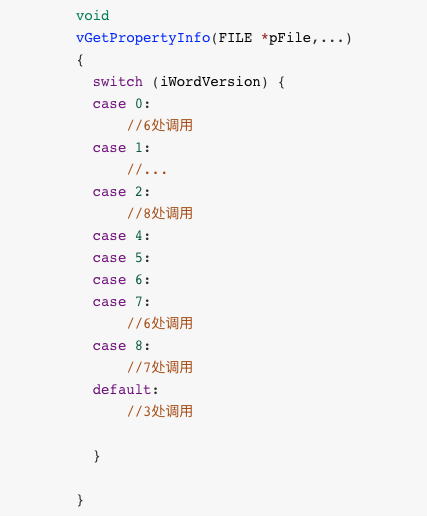
\includegraphics[width = 0.5\textwidth]{扇出高例子.jpg}
\caption{vGetPropertyInfo方法结构}
\end{figure}
    

这里以antiword项目中properties.c文件的vGetPropertyInfo方法为例,该方法主要根据传入的Word版本,从文档中提取各种属性信息。该方法的扇出度为30,是项目中扇出度较大的一个,方法可能复杂度过高,因此被报告属于不良的扇出,但这一报告并未得到用户的接受。其原因在于,该方法的核心结构是一个包含多达9种不同情况的 switch 语句,每种情况又细分为多个子情况,因此导致总共产生了30个方法调用。该方法的合理性在于通过清单式方式集中处理所有功能逻辑,使得用户能够一目了然。此设计不仅减少了冗余代码,避免了方法调用链过长带来的可读性问题,还降低了因方法调用所带来的额外开销,从而优化了整体系统的效率。因此,尽管该方法具有较高的扇出度,其设计思路仍然是有效的,符合高效代码的要求。

(3)静态工具检测接受率分析

静态工具检验得到的代码缺陷的接受率是最高的,经过分析发现只有个别错误,如平台相关问题,与特定编译器相关的警告等不容易被开发者所接受,因为这并不是代码本身的质量问题。


经过分析可以发现,这些度量指标有一定的有效性,但是这些度量聚焦的往往是范围较小的质量问题。如模块内、方法内甚至语句级的质量问题。面对更大规模的软件代码时,无法反映其在架构上的缺陷,难以帮助开发者从宏观的角度上指导代码维护。


2. 代码审查图

(1)代码审查图概览

图 4-4 展示了 Antiword 项目和 TheAlgorithms 项目的代码审查图,直观地反映了两者的结构特征和模块化差异。图中,圆形节点表示方法,方形节点表示全局变量,不同颜色的边则代表了代码元素之间的不同关系:蓝色边表示依赖关系,绿色边表示耦合关系,红色边表示代码变更影响关系。上方的图是未区分模块的全局视图,所有的节点和边混杂在一起,仅从整体上体现了项目的结构复杂度。而下方的图对模块进行了区分,采用颜色区分不同模块,将属于同一模块的节点用相同颜色进行标注,从而进一步突出模块之间的边界和逻辑关系。

\begin{figure}[!h]
    \setlength{\subfigcapskip}{-1bp}
    \centering
    \begin{minipage}{\textwidth}
    \centering
    \subfigure[antiword-未划分模块]{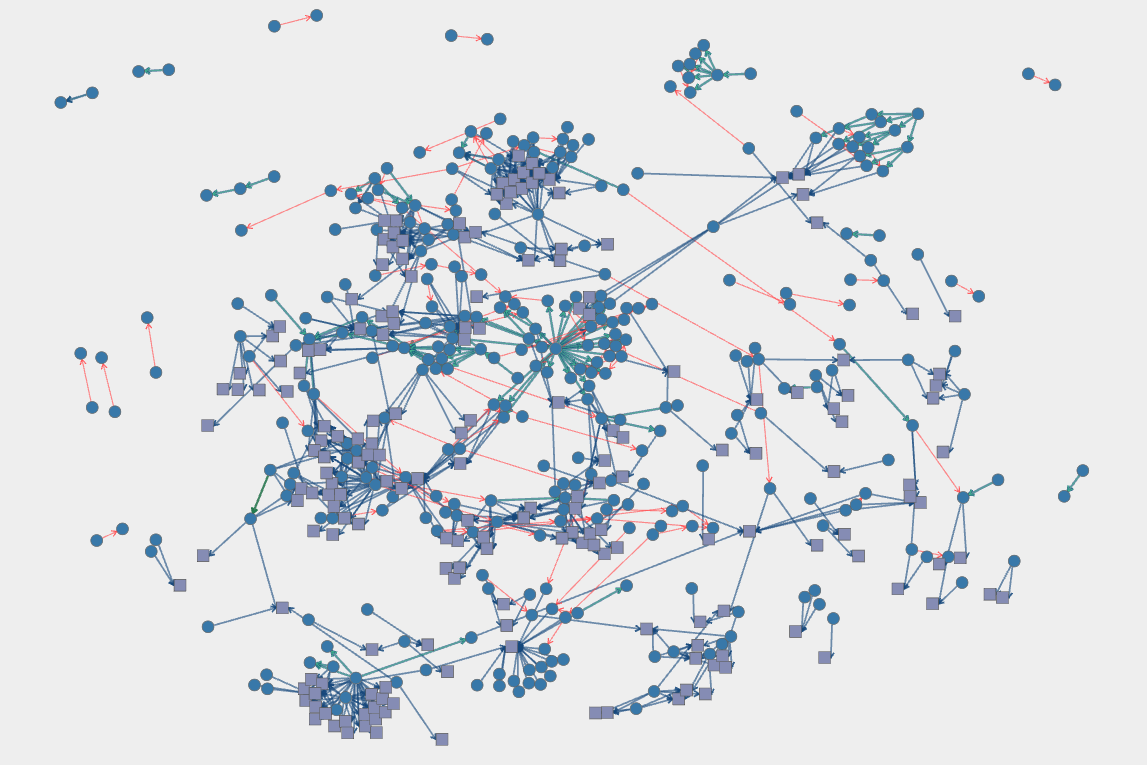
\includegraphics[width=0.4\textwidth]{antiword审查图未上色.jpg}} % 保留中文标题
    \hspace{2em}
    \subfigure[TheAlgorithms-未划分模块]{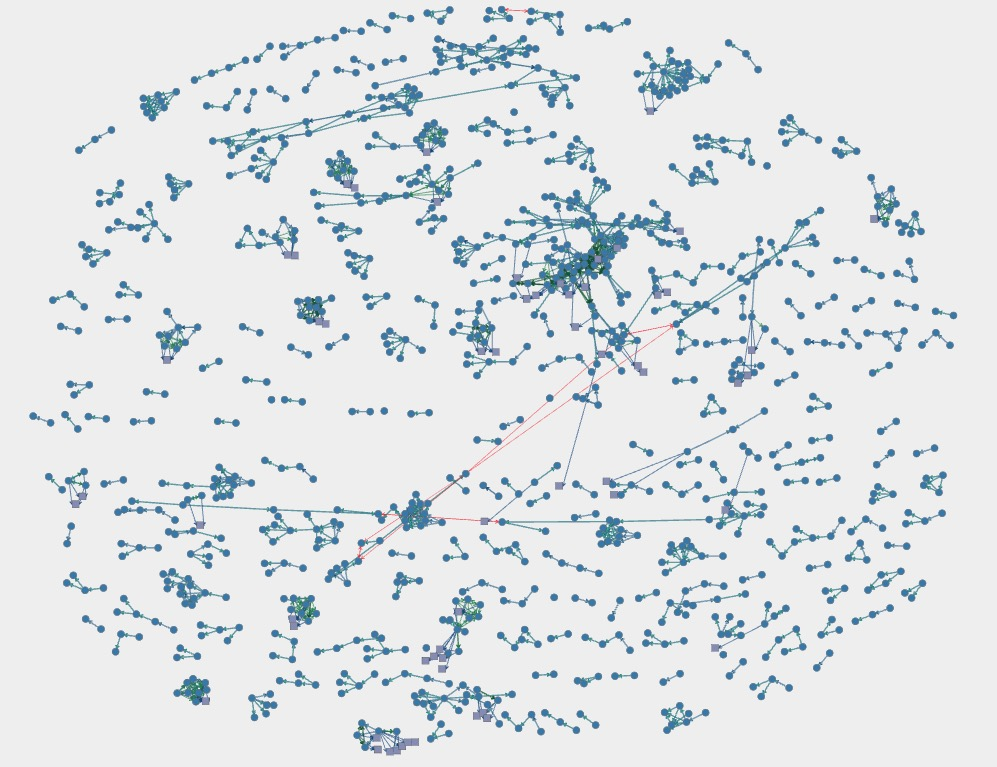
\includegraphics[width=0.4\textwidth]{aigri代码审查图-未上色.jpg}} % 保留中文标题
    \end{minipage}
    \centering
    \begin{minipage}{\textwidth}
    \centering
    \subfigure[antiword-划分模块]{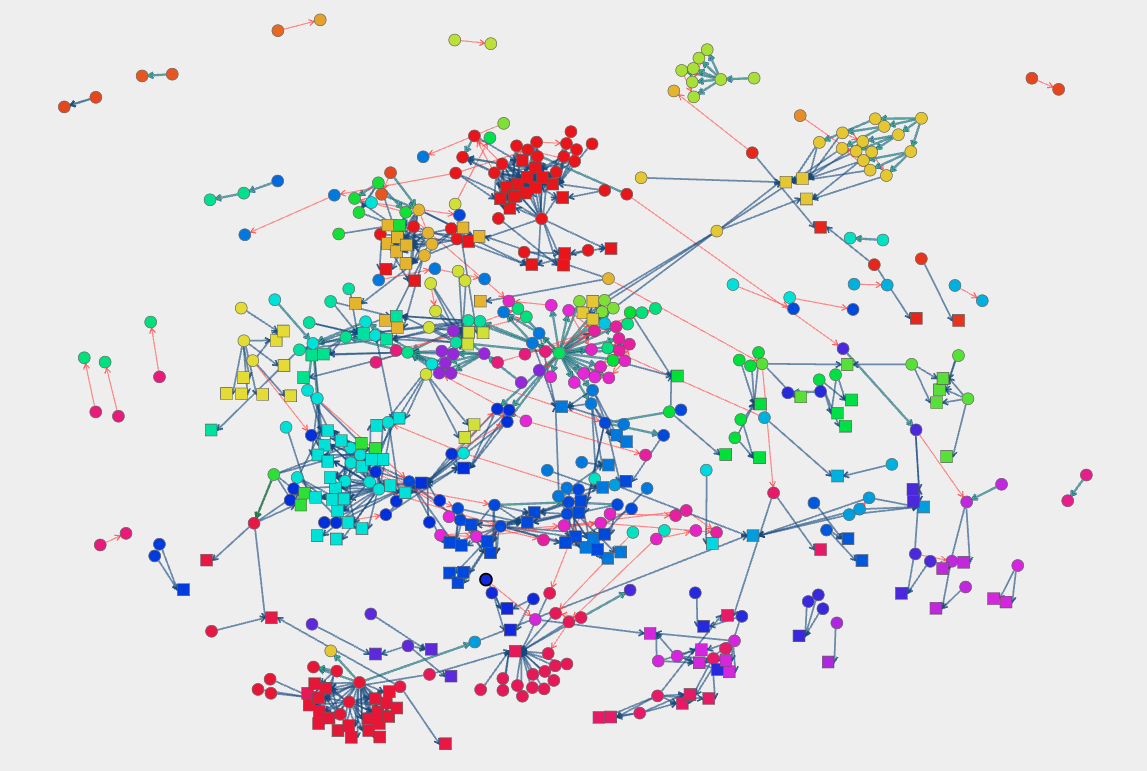
\includegraphics[width=0.4\textwidth]{antiword代码审查图.jpg}} % 保留中文标题
    \hspace{2em}
    \subfigure[TheAlgorithms-划分模块]{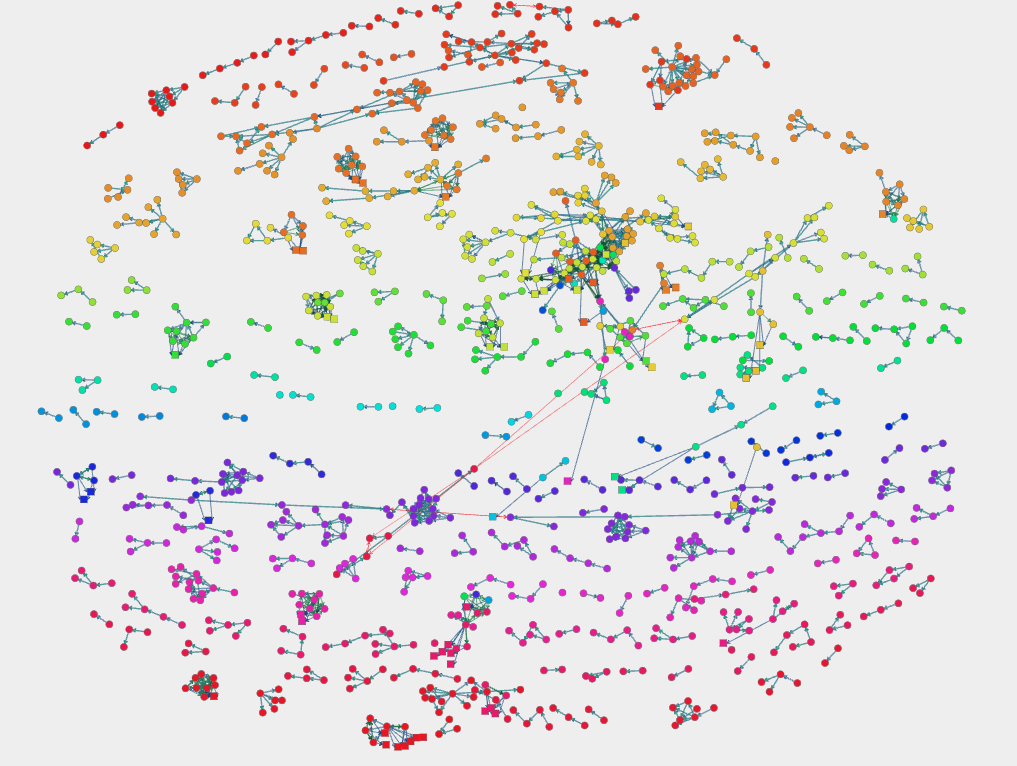
\includegraphics[width=0.4\textwidth]{aigri代码审查图.jpg}} % 保留中文标题
    \end{minipage}
    \vspace{0.2em}
    \caption{代码审查图} % 只保留中文标题
\end{figure}


从图中可以明显看出两个项目在结构特征上的显著差异。Antiword 项目整体模块之间高度协作,共同实现一个完整的功能,因此模块之间的联系较为紧密,表现出较强的耦合性。从可视化图上观察,按模块划分后,可以清晰地看到具有相同功能的模块形成了较为紧密的聚集。同一颜色的节点集中分布,进一步体现了模块的内聚性较高以及逻辑结构的清晰性。

相比之下,TheAlgorithms 项目由于其作为算法库的特性,方法之间的耦合性较低,各模块间的联系相对较弱。从图上来看,不同模块呈现出较为分散的分布,模块内部的聚集程度也较低。整体结构表现为由若干独立模块组成,松散而分离,符合库函数式项目的典型特征。

\begin{figure}[h]
\centering
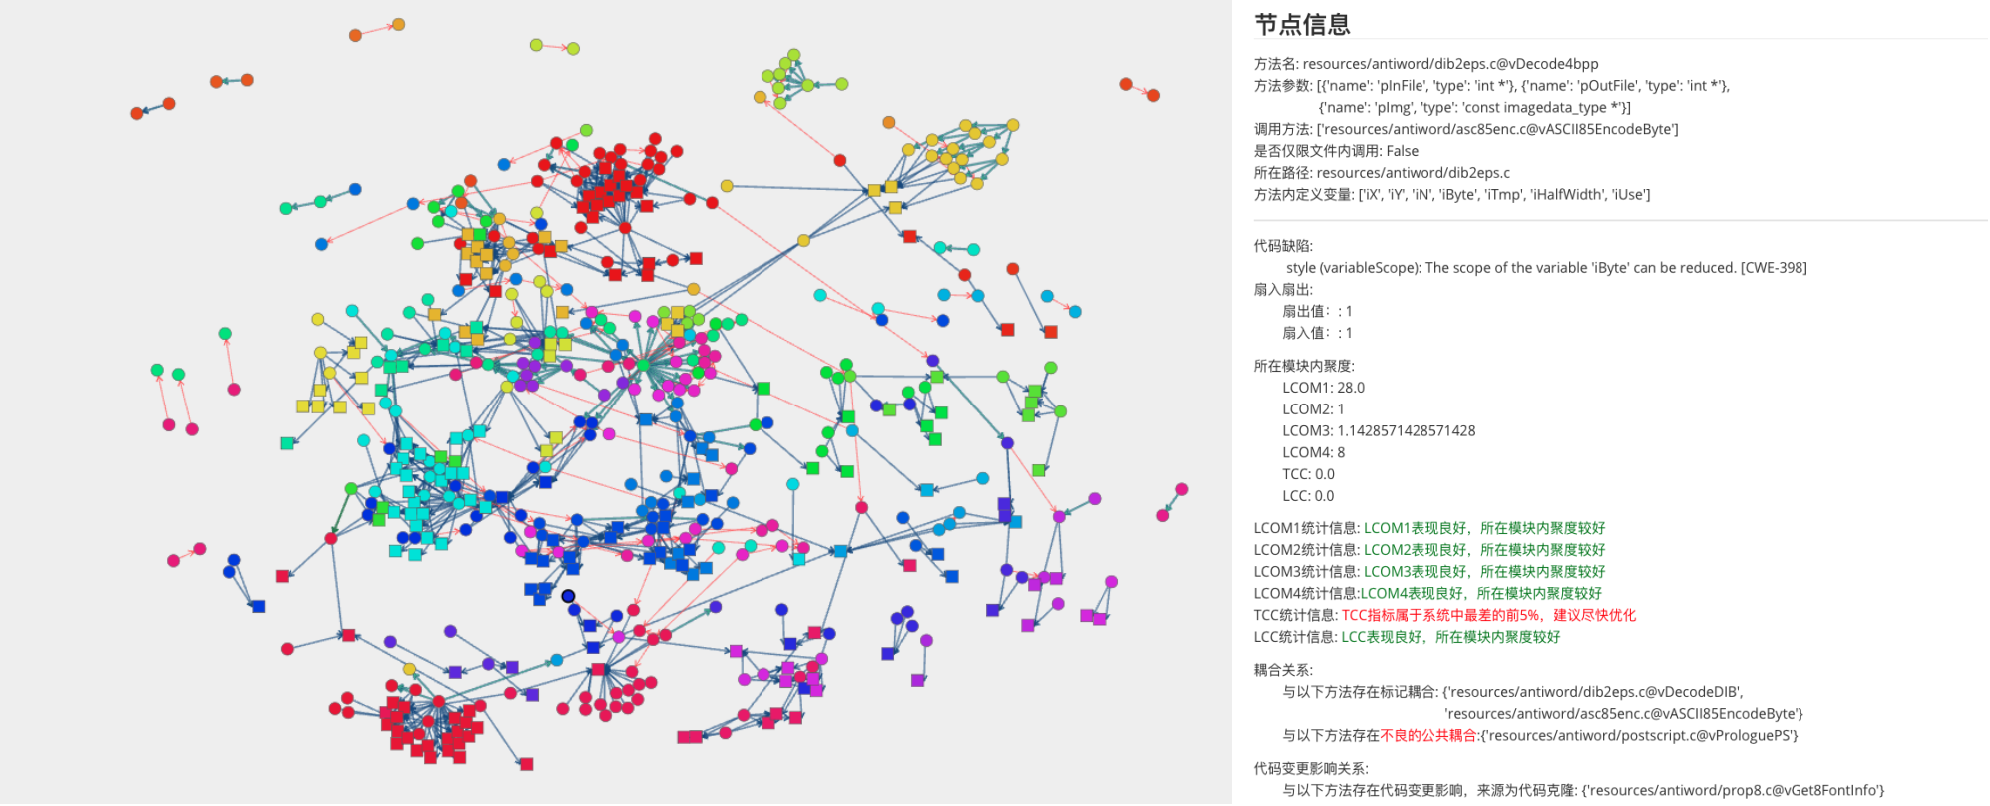
\includegraphics[width = 1\textwidth]{点击节点.png}
\caption{点击节点展开节点信息}
\end{figure}

此外,用户可以通过点击图中的某个节点来查看该节点的详细信息,包括方法或全局变量的具体描述。这一功能能够帮助用户快速定位关键信息,深入了解特定方法或变量的功能和用途,从而更高效地进行代码审查和理解。



(2)子图展示

代码审查图蕴含了丰富且有价值的信息,通过聚焦于代码审查图中的子图,开发者和审查者可以快速直观地理解代码结构之间的关系。子图清晰地展示了代码结构之间的依赖、耦合以及变更影响关系,使得复杂的代码逻辑更加可视化。

以 antiword 项目中的子图为例,本文聚焦于 vDecodeDIB 方法的代码开发和审查场景。若按照传统方法对该方法进行开发或分析,仅通过人工阅读代码,开发者需要深入解析与其相关的依赖关系和变更影响关系,这可能涉及 300 多行代码的逻辑才能全面掌握方法的上下文。然而,通过代码审查图,开发者只需关注 8 个节点和 9 条边,即可快速获取关键信息。这种直观的可视化显著降低了代码理解的复杂度和成本。

\begin{figure}[h]
\centering
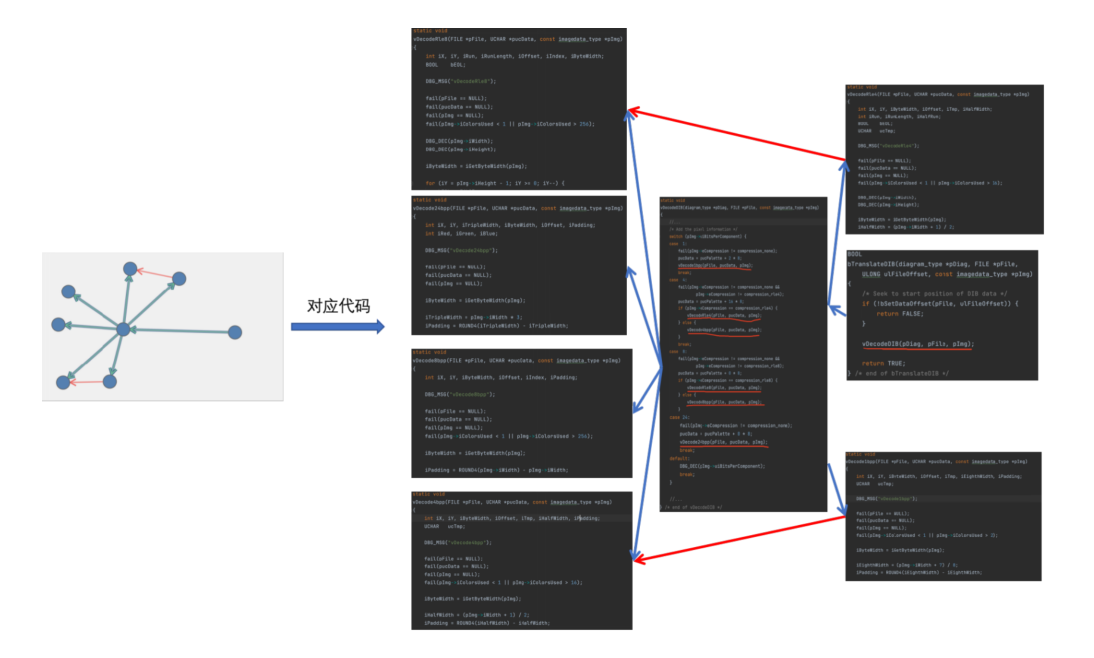
\includegraphics[width = 1\textwidth]{代码审查图子图.jpg}
\caption{vDecodeDIB方法上下文}
\end{figure}

尤其值得注意的是,变更影响关系中包含了两个基于克隆代码的关系。这类关系通常隐匿于代码中,开发者仅靠手动查看代码很难准确发现并记录。代码审查图将这些隐藏的克隆关系显式标出,使开发者在代码修改时能够快速识别潜在的影响范围,从而避免遗漏变更的风险。

对开发者而言,代码审查图能够提供更加直观的视角,帮助其快速掌握代码之间的各种依赖关系和耦合情况。在代码开发过程中,审查图不仅有助于理清模块间的关系,还能有效避免变更不完全的问题。而对于代码审查者,审查图能够快速展示代码的上下文结构,简化复杂逻辑的理解过程,同时高效地识别代码中的变更缺陷。

(3)代码质量属性体现

通过代码审查图,不仅可以直观展示代码的依赖关系和变更影响关系,还能有效地体现代码质量的特征,从而辅助用户理解代码质量较差或较好的具体原因。在第 2.6.2 节中详细解释了 misc.c 文件内聚度表现最差的原因,并统计了该文件内部方法和变量的相关信息。然而,仅依靠文字说明可能难以全面传达问题的全貌,而配合代码审查图,如图4-7所示,可以更加直观地展示该模块的结构问题。

\begin{figure}[h]
\centering
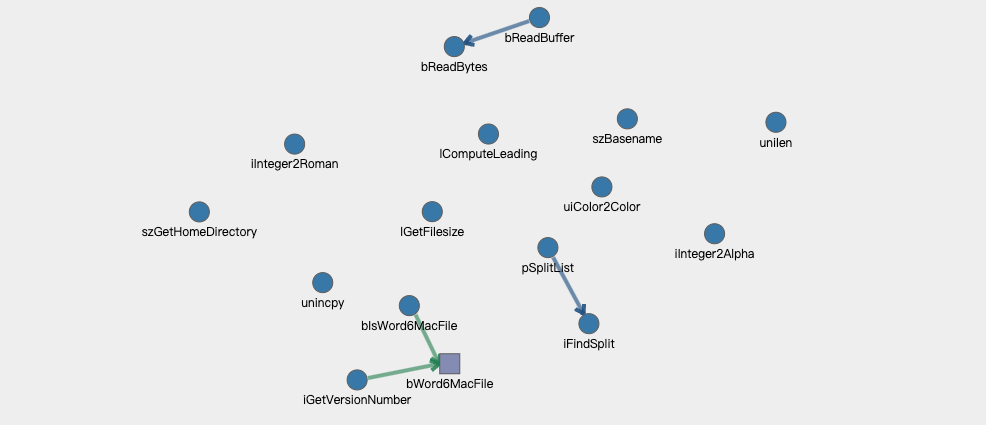
\includegraphics[width = 0.7\textwidth]{内聚度差例子.jpg}
\caption{misc.c 文件对应的代码审查图}
\end{figure}

从图中可以清晰地看出,misc.c 文件的结构非常松散,其内部存在大量孤立节点,缺乏足够的联系和协调关系。这些孤立节点既无法与其他节点形成有意义的逻辑关系,也难以体现出模块内部的高内聚性特征。这种松散的结构正是导致其内聚度表现最差的主要原因。

除此之外还有一些内聚度差和好的模块在代码审查图中可以清晰地展现,如图4-8所示。图中,左侧展示的是内聚度较差的模块,而右侧则展示了内聚度较好的模块。单纯从代码本身出发,往往难以直观地识别出导致内聚度差或较好的具体原因。然而,通过代码审查图,问题的根源得以清晰呈现。具体来说,左侧内聚度差的模块之所以表现为低内聚度,主要是因为存在过多的链式调用,这种设计使得模块之间的依赖关系过于松散,缺乏足够的内在联系。而右侧内聚度良好的模块,则表现出较强的模块化特征,模块内部功能紧密相关,依赖关系清晰且有序,从而促进了代码的高内聚性。通过这种可视化的方式,代码审查图不仅帮助开发者迅速识别出模块内聚度的优劣,还能够为后续的重构与优化提供建议,如左侧内聚度差的模块,可通过合并方法,减少方法数和调用量,达到提高内聚度的效果。

\begin{figure}[!h]
    \setlength{\subfigcapskip}{-1bp}
    \centering
    \begin{minipage}{\textwidth}
    \centering
    \subfigure[内聚度差——存在链式调用]{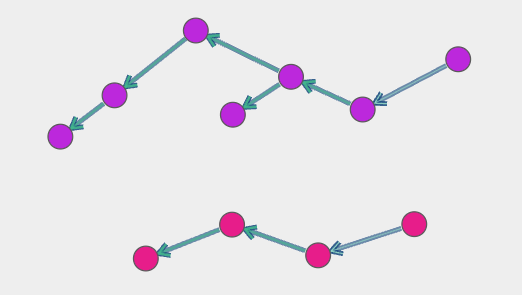
\includegraphics[width=0.4\textwidth]{存在链式调用.jpg}} % 保留中文标题
    \hspace{2em}
    \subfigure[内聚度良好——关联紧密]{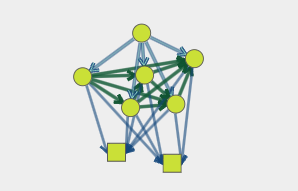
\includegraphics[width=0.4\textwidth]{内聚度好.jpg}} % 保留中文标题
    \end{minipage}
    \vspace{0.2em}
    \caption{内聚度良好和较差的例子} % 只保留中文标题
\end{figure}


在2.6.2节中对高扇出方法的讨论中,高扇出通常意味着方法存在过高的复杂性,这种特征在代码审查图中表现为具有大量的出边的中心化节点。如图4-9所示。图中的中心节点通过大量出边与其他模块或方法产生关联,这种结构不仅揭示了方法的复杂性,也反映了其可能导致的维护难度和潜在的设计缺陷。用户可以通过代码审查图迅速定位到具有高扇出的具体方法,深入了解其上下文信息,进而判断其是否存在不合理的复杂度。当发现高扇出的原因主要源于过多的依赖关系时,开发者可以及时采取相应的优化措施,如重构该方法、简化其职责或调整其与其他模块的关系,从而有效提升系统的可维护性和可扩展性。

\begin{figure}[h]
\centering
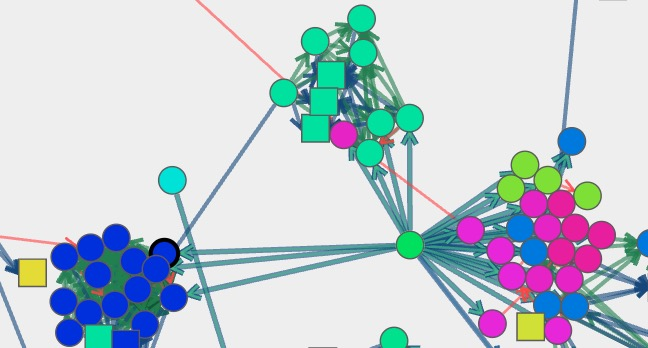
\includegraphics[width = 0.4\textwidth]{扇出度最高.jpg}
\caption{扇出度较高的节点}
\end{figure}

对于某些方法,其功能可能已经与当前所在模块的职责不再完全匹配,而与其他模块的结合更加紧密。这一问题在代码审查图中得以有效呈现。得益于力导向图的可视化特性,图中会显示出方法之间的依赖关系与耦合关系,紧密依赖的节点往往聚集在一起。由于同一模块内的节点通常会被赋予相同的颜色,若模块划分不合理,则会出现如图4-10所示的情况。在图中,聚集的节点颜色并不统一,某些节点(如图中的绿色和蓝色节点)与模块的主色调(橙色)不符。这表明,尽管这些方法本应属于其他模块,但它们与当前模块(即橙色模块)之间的耦合关系更为紧密。通过这种可视化,用户能够明确识别出不合理的模块划分,并采取相应的重构措施,例如将这些方法迁移至更合适的模块中,避免产生不良的耦合关系。这种调整不仅能够优化模块的功能划分,还能提高系统的可维护性与可扩展性,减少未来修改时的复杂度。


\begin{figure}[h]
\centering
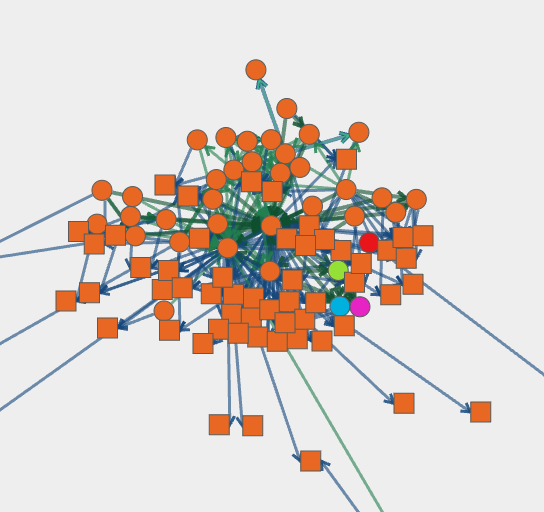
\includegraphics[width = 0.4\textwidth]{模块分错.jpg}
\caption{模块划分不合适的方法}
\end{figure}


在代码审查图中,我们也能看到一些方法之间的不良变更影响关系。除了直接反映变更影响较多的方法外,代码审查图还能够揭示出由于变更影响分析所导致的模块间不良变更传播问题。如图4-11。该子图涉及三个模块,每个模块的内聚度均较为良好,然而每个模块内都有一个方法与其他两个模块之间存在变更影响关系。这导致当这几个方法变动时,可能影响到不属于同一模块的代码也要跟着改变。更为严重的是,随着变更的涟漪效应,这些变更会进一步扩散,影响到更多模块,造成不必要的连锁反应。这种现象揭示了该系统架构存在潜在的问题——尽管各模块内部结构较为合理,但模块之间的依赖关系过于复杂且紧密,增加了维护和变更时的复杂度和风险。为解决这一问题,优化的建议是尽量减少或消除这种不良的变更影响关系。具体而言,可以通过提取和复用模块间的共同代码逻辑,消除不必要的代码克隆,进而降低跨模块变更传播的可能性。


\begin{figure}[h]
\centering
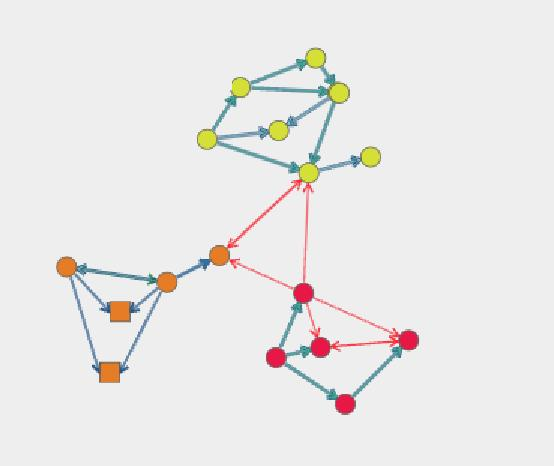
\includegraphics[width = 0.4\textwidth]{变更影响关系审查图.jpg}
\caption{不良的变更影响关系}
\end{figure}


总而言之,通过代码审查图,不仅能够帮助开发者快速定位模块质量问题,还能直观地理解问题的根源,为后续的优化和改进提供清晰的建议。这种结合文字与图形的分析方式,显著提升了代码质量评估的直观性和说服力。

3. 代码质量评估报告

下图展示了一个实际的代码评估报告示例。由于报告内容较长,这里仅展示了其中的一部分信息。通过代码评估报告,用户能够以结构化的清单形式全面了解软件项目中存在的各类质量问题及其具体位置。这些报告不仅清晰地列出了每个问题的详细描述,还提供了针对性优化或重构的建议。通过这种方式,开发团队可以快速识别代码中的潜在缺陷或性能瓶颈,并根据报告中提供的指导意见,采取有效的措施进行改进。报告的可视化和条目化呈现,帮助用户直观地理解各项问题的优先级和重要性,从而优化项目的维护流程,并提高软件系统的整体质量。

\clearpage

\begin{figure}[h]
\centering
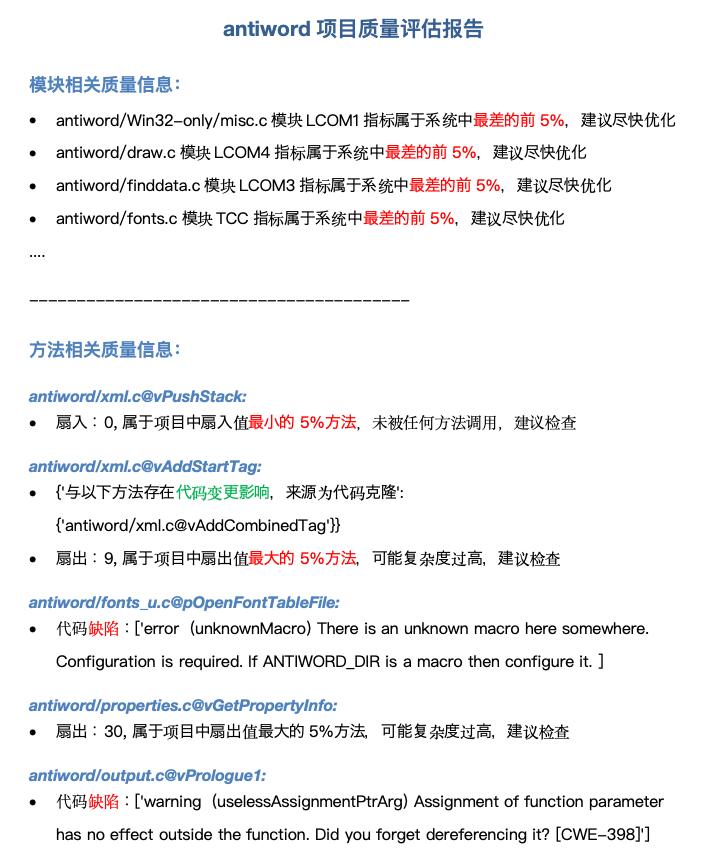
\includegraphics[width = 1.0\textwidth]{质量评估报告.jpg}
\caption{antiword项目代码质量评估报告节选}
\end{figure}


\section{代码审查图的实际应用}

在实际应用中,代码审查图可以有以下三种用法。

\paragraph{辅助开发者的代码维护} 当用户对软件代码进行开发时,可将复杂庞大的项目先通过系统进行分析,得到代码审查图。

\begin{figure}[h]
\centering
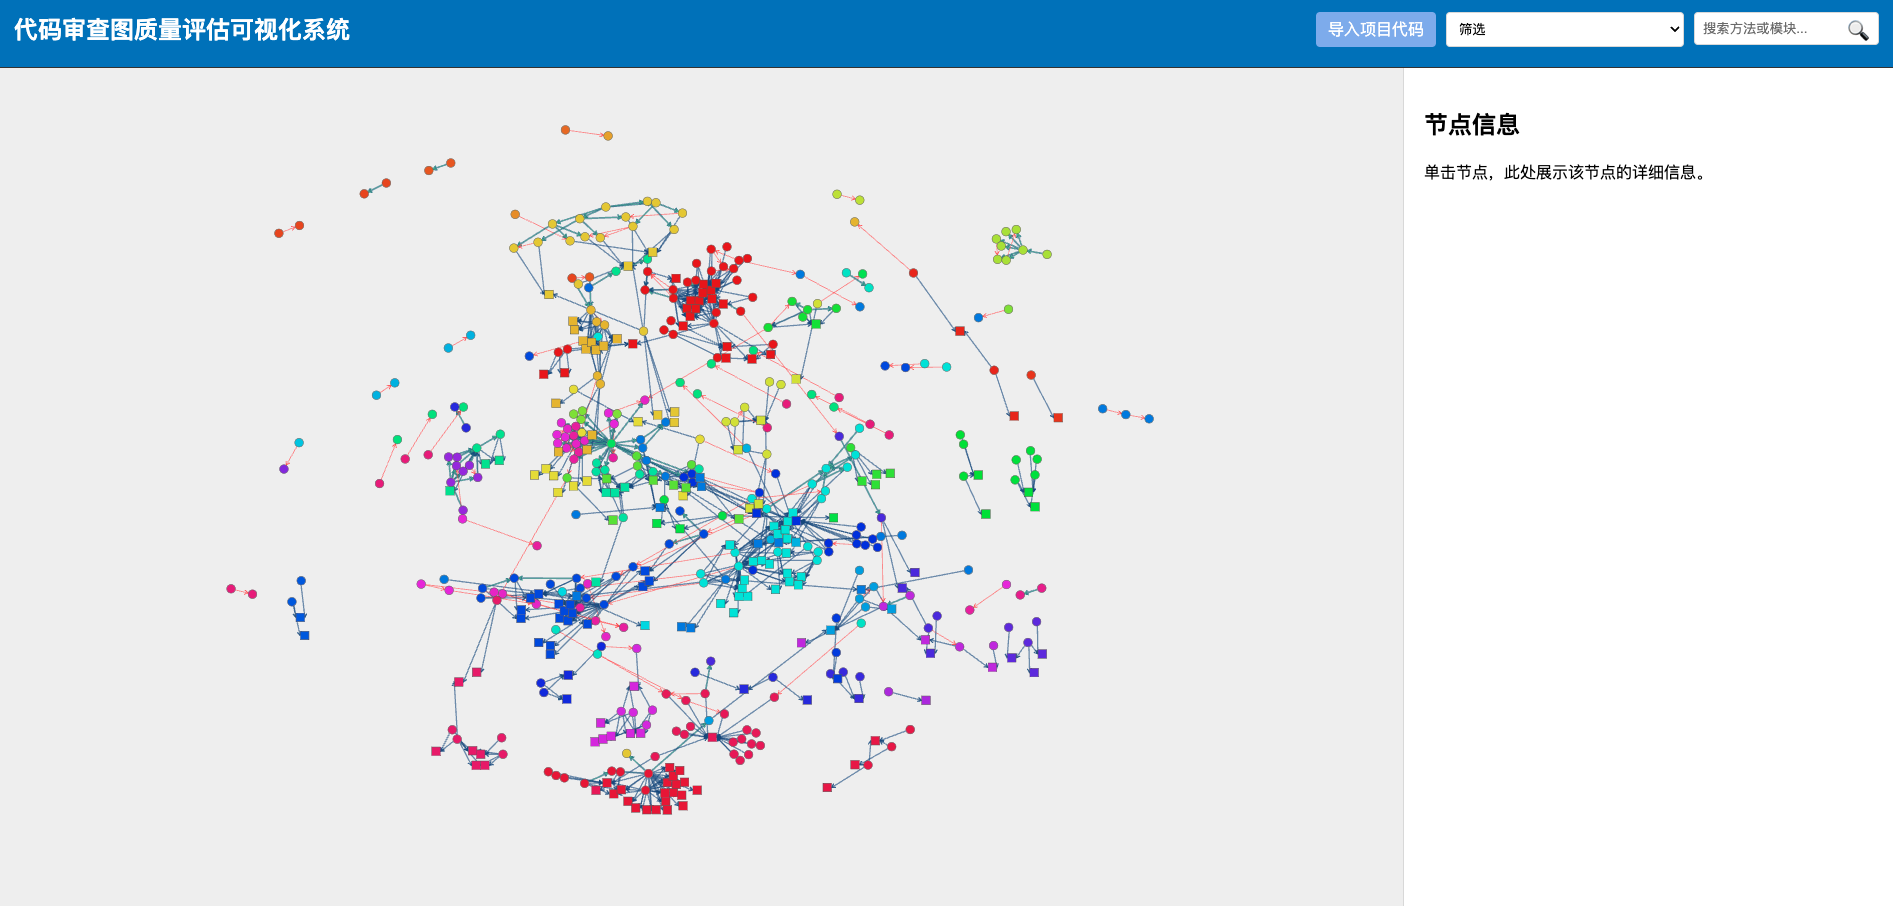
\includegraphics[width = 1.0\textwidth]{应用展示审查图.jpg}
\caption{导入项目生成代码审查图}
\end{figure}

对于开发任务所在的代码上下文,通过搜索方法名找到其在代码审查图中的位置,点击节点查看方法详细信息和质量情况,用户可根据相应的建议进行修改,优化代码质量。

\begin{figure}[h]
\centering
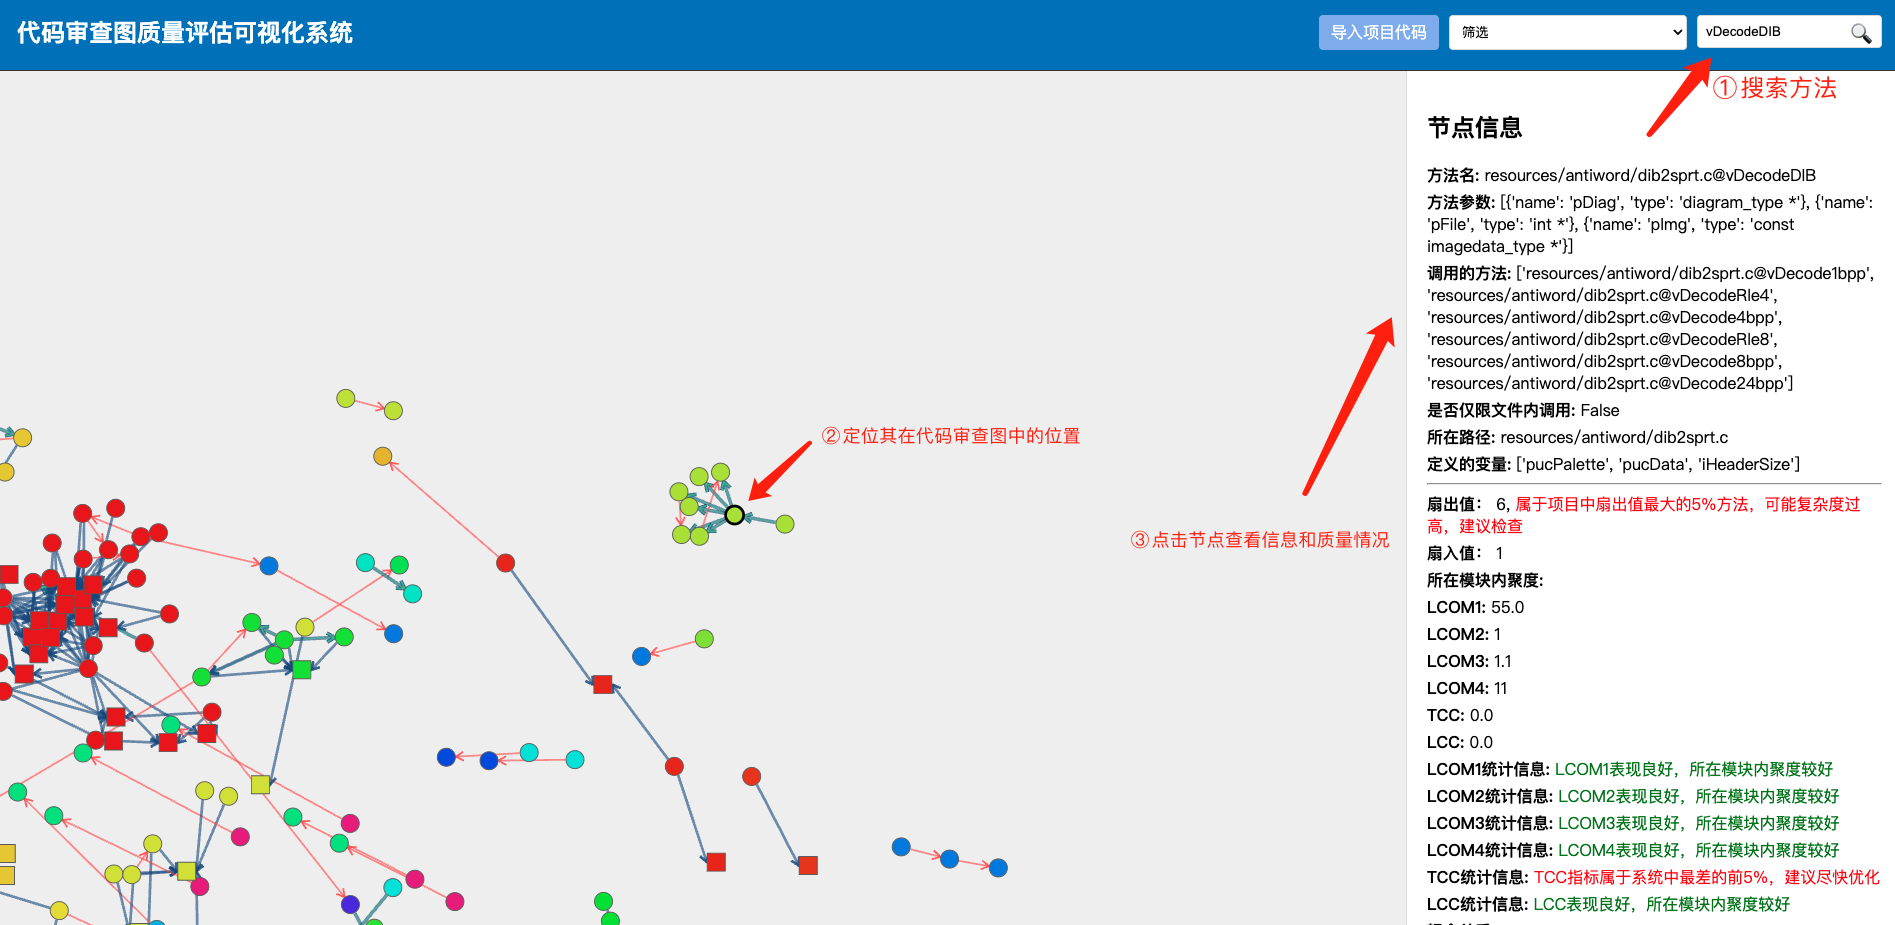
\includegraphics[width = 1.0\textwidth]{应用查看节点信息.jpg}
\caption{定位开发任务涉及的方法,查看质量信息}
\end{figure}

根据代码审查图的边,则可以了解当前代码与其他部分的依赖关系、耦合关系和变更影响关系。尤其是变更影响关系,可以帮助用户在进行变更时,提示其依赖型和逻辑型影响的范围,并根据给出的建议,帮助用户安全变更,解决了用户面对复杂软件难以理解、不敢变更、容易变更不完全的痛点。

\begin{figure}[h]
\centering
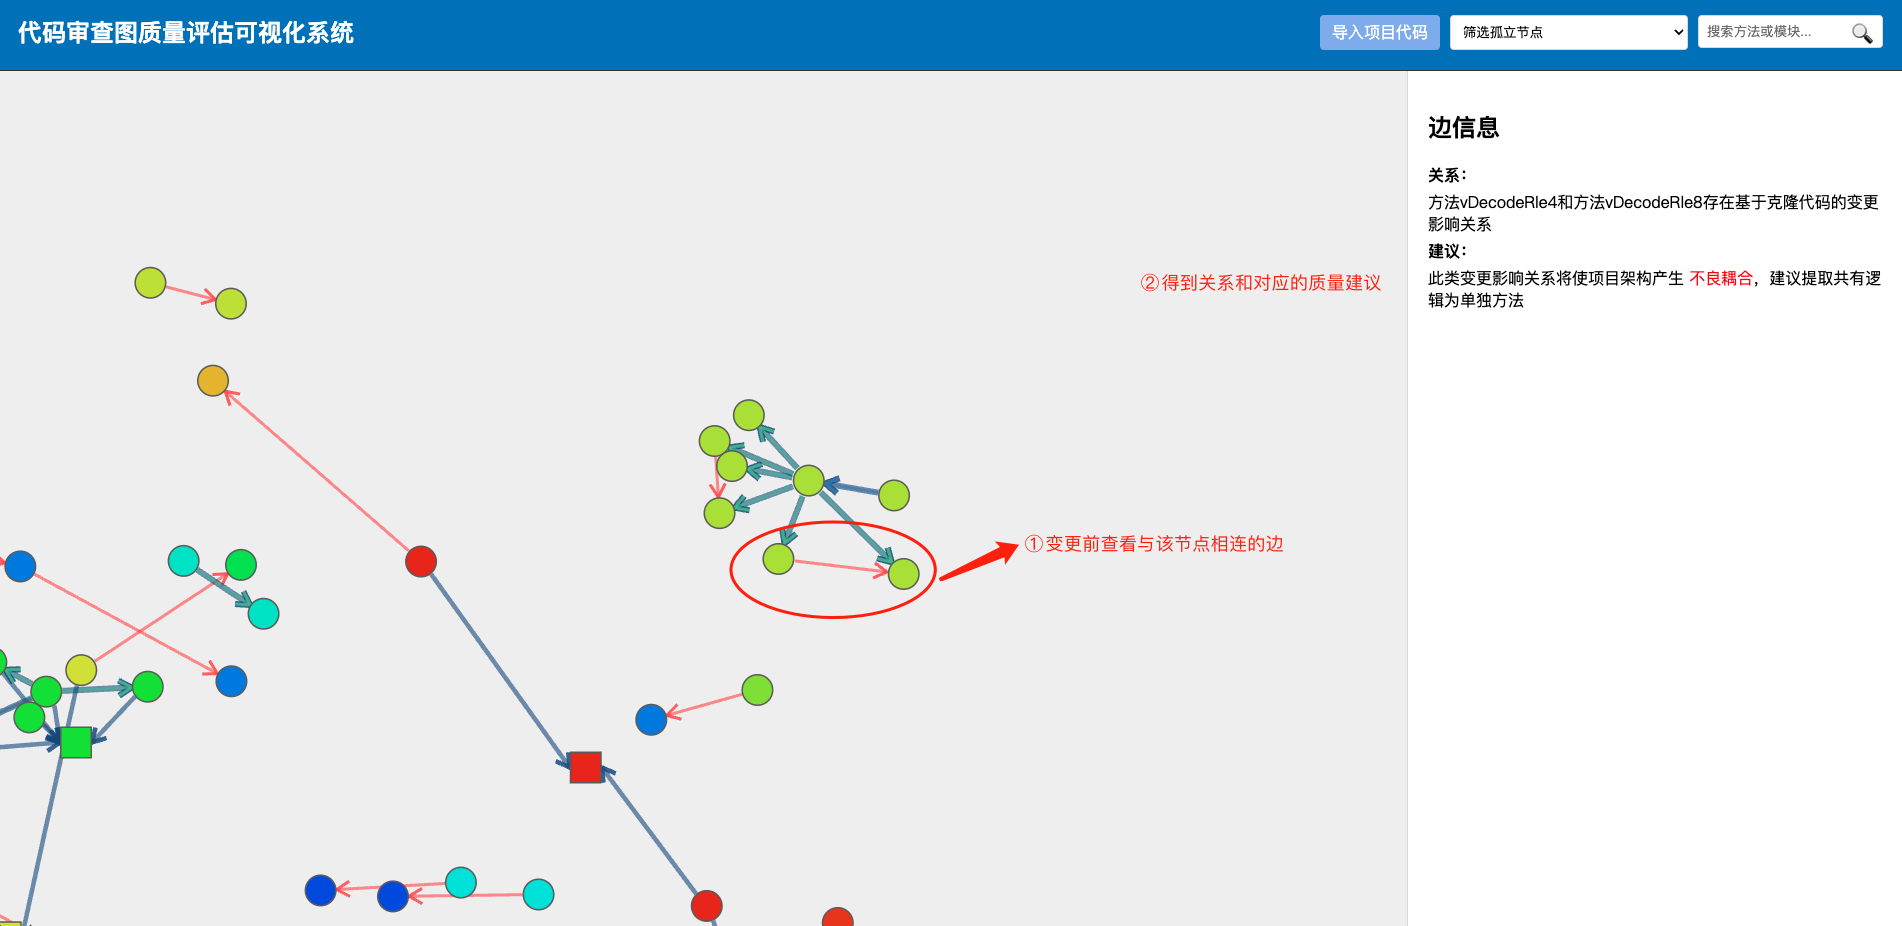
\includegraphics[width = 1.0\textwidth]{应用边信息.jpg}
\caption{查看方法对应边,按建议安全变更}
\end{figure}

\paragraph{作为审查工具帮助审查者进行审查} 当面对审查任务时,审查者可通过搜索代码审查图定位到当前提交所涉及的节点,通过图中的关系迅速了解代码上下文间的调用以及变更影响关系,通过系统的提示,对开发者的变更进行审查,检查其功能逻辑上是否安全变更,检查其变更操作给软件带来的质量影响是恶化还是优化,从而给出对应的审查结果。

\paragraph{作为质量评估工具对软件代码进行整体的评估} 用户可根据代码审查图,观察软件模块划分,也可导出代码质量评估报告,以清单的方式了解项目代码的质量情况。



\section{本章小结}

本章介绍了基于标签生成的方法模块分类,该方法通过大语言模型生成方法的实际标签进行分类,表明模块划分不正确的方法,通过实验证明,该方法具有一定的参考意义。其次介绍了代码审查图,将软件分析结果以图的形式展示给用户,方便用户从宏观的角度了解项目结构,最后介绍了代码质量报告的生成,通过清单式的质量信息报告,方便用户查询和优化。

\backmatter
% !Mode:: "TeX:UTF-8" 
\begin{conclusions}

学位论文的结论作为论文正文的最后一章单独排写,但不加章标题序号。

结论应是作者在学位论文研究过程中所取得的创新性成果的概要总结,不能与摘要混为一谈。博士学位论文结论应包括论文的主要结果、创新点、展望三部分,在结论中应概括论文的核心观点,明确、客观地指出本研究内容的创新性成果(含新见解、新观点、方法创新、技术创新、理论创新),并指出今后进一步在本研究方向进行研究工作的展望与设想。对所取得的创新性成果应注意从定性和定量两方面给出科学、准确的评价,分(1)、(2)、(3)…条列出,宜用“提出了”、“建立了”等词叙述。

\end{conclusions}
   % 结论
\bibliographystyle{gbt7714-numerical}
% \bibliographystyle{hitszthesis} % 深圳校区的同学请使用 hitszthesis 文献样式
%\bibliographystyle{hithesis} %理论上2020最新要求文献样式GB/T 7714—2015,但若院系要求文献英文作者不全大写,可改用hithesis文献样式
%%%%%%%%%%%%%%%%%%%%%%%%%%%%%%%%%%%%%%%%%%%%%%%%%%%%%%%%%%%%%%%%%%%%%%%%%%%%%%%%
%-- 注意:以下本硕博、博后书序不一致 --%
%%%%%%%%%%%%%%%%%%%%%%%%%%%%%%%%%%%%%%%%%%%%%%%%%%%%%%%%%%%%%%%%%%%%%%%%%%%%%%%%
% 本科书序(哈尔滨、深圳校区)
%%%%%%%%%%%%%%%%%%%%%%%%%%%%%%%%%%%%%%%%%%%%%%%%%%%%%%%%%%%%%%%%%%%%%%%%%%%%%%%%
% \bibliography{reference} % 参考文献
% \authorization %授权
% % \authorization[scan.pdf] %添加扫描页的命令,与上互斥
% % !Mode:: "TeX:UTF-8"
\begin{acknowledgements}



\end{acknowledgements}
 %致谢
% \begin{appendix}%附录
% \chapter{外文资料原文}
\label{cha:engorg}

\title{The title of the English paper}

\textbf{Abstract:} As one of the most widely used techniques in operations
research, \emph{ mathematical programming} is defined as a means of maximizing a
quantity known as \emph{bjective function}, subject to a set of constraints
represented by equations and inequalities. Some known subtopics of mathematical
programming are linear programming, nonlinear programming, multiobjective
programming, goal programming, dynamic programming, and multilevel
programming$^{[1]}$.

It is impossible to cover in a single chapter every concept of mathematical
programming. This chapter introduces only the basic concepts and techniques of
mathematical programming such that readers gain an understanding of them
throughout the book$^{[2,3]}$.


\section{Single-Objective Programming}
The general form of single-objective programming (SOP) is written
as follows,
\begin{equation}\tag*{(123)} % 如果附录中的公式不想让它出现在公式索引中,那就请
                             % 用 \tag*{xxxx}
\left\{\begin{array}{l}
\max \,\,f(x)\\[0.1 cm]
\mbox{subject to:} \\ [0.1 cm]
\qquad g_j(x)\le 0,\quad j=1,2,\cdots,p
\end{array}\right.
\end{equation}
which maximizes a real-valued function $f$ of
$x=(x_1,x_2,\cdots,x_n)$ subject to a set of constraints.

\newtheorem{mpdef}{Definition}[chapter]
\begin{mpdef}
In SOP, we call $x$ a decision vector, and
$x_1,x_2,\cdots,x_n$ decision variables. The function
$f$ is called the objective function. The set
\begin{equation}\tag*{(456)} % 这里同理,其它不再一一指定。
S=\left\{x\in\Re^n\bigm|g_j(x)\le 0,\,j=1,2,\cdots,p\right\}
\end{equation}
is called the feasible set. An element $x$ in $S$ is called a
feasible solution.
\end{mpdef}

\newtheorem{mpdefop}[mpdef]{Definition}
\begin{mpdefop}
A feasible solution $x^*$ is called the optimal
solution of SOP if and only if
\begin{equation}
f(x^*)\ge f(x)
\end{equation}
for any feasible solution $x$.
\end{mpdefop}

One of the outstanding contributions to mathematical programming was known as
the Kuhn-Tucker conditions\ref{eq:ktc}. In order to introduce them, let us give
some definitions. An inequality constraint $g_j(x)\le 0$ is said to be active at
a point $x^*$ if $g_j(x^*)=0$. A point $x^*$ satisfying $g_j(x^*)\le 0$ is said
to be regular if the gradient vectors $\nabla g_j(x)$ of all active constraints
are linearly independent.

Let $x^*$ be a regular point of the constraints of SOP and assume that all the
functions $f(x)$ and $g_j(x),j=1,2,\cdots,p$ are differentiable. If $x^*$ is a
local optimal solution, then there exist Lagrange multipliers
$\lambda_j,j=1,2,\cdots,p$ such that the following Kuhn-Tucker conditions hold,
\begin{equation}
\label{eq:ktc}
\left\{\begin{array}{l}
    \nabla f(x^*)-\sum\limits_{j=1}^p\lambda_j\nabla g_j(x^*)=0\\[0.3cm]
    \lambda_jg_j(x^*)=0,\quad j=1,2,\cdots,p\\[0.2cm]
    \lambda_j\ge 0,\quad j=1,2,\cdots,p.
\end{array}\right.
\end{equation}
If all the functions $f(x)$ and $g_j(x),j=1,2,\cdots,p$ are convex and
differentiable, and the point $x^*$ satisfies the Kuhn-Tucker conditions
(\ref{eq:ktc}), then it has been proved that the point $x^*$ is a global optimal
solution of SOP.

\subsection{Linear Programming}
\label{sec:lp}

If the functions $f(x),g_j(x),j=1,2,\cdots,p$ are all linear, then SOP is called
a {\em linear programming}.

The feasible set of linear is always convex. A point $x$ is called an extreme
point of convex set $S$ if $x\in S$ and $x$ cannot be expressed as a convex
combination of two points in $S$. It has been shown that the optimal solution to
linear programming corresponds to an extreme point of its feasible set provided
that the feasible set $S$ is bounded. This fact is the basis of the {\em simplex
  algorithm} which was developed by Dantzig as a very efficient method for
solving linear programming.
\begin{table}[ht]
\centering
  \centering
  \caption*{Table~1\hskip1em This is an example for manually numbered table, which
    would not appear in the list of tables}
  \label{tab:badtabular2}
  \begin{tabular}[c]{|m{1.5cm}|c|c|c|c|c|c|}\hline
    \multicolumn{2}{|c|}{Network Topology} & \# of nodes &
    \multicolumn{3}{c|}{\# of clients} & Server \\\hline
    GT-ITM & Waxman Transit-Stub & 600 &
    \multirow{2}{2em}{2\%}&
    \multirow{2}{2em}{10\%}&
    \multirow{2}{2em}{50\%}&
    \multirow{2}{1.2in}{Max. Connectivity}\\\cline{1-3}
    \multicolumn{2}{|c|}{Inet-2.1} & 6000 & & & &\\\hline
    & \multicolumn{2}{c|}{ABCDEF} &\multicolumn{4}{c|}{} \\\hline
\end{tabular}
\end{table}

Roughly speaking, the simplex algorithm examines only the extreme points of the
feasible set, rather than all feasible points. At first, the simplex algorithm
selects an extreme point as the initial point. The successive extreme point is
selected so as to improve the objective function value. The procedure is
repeated until no improvement in objective function value can be made. The last
extreme point is the optimal solution.

\subsection{Nonlinear Programming}

If at least one of the functions $f(x),g_j(x),j=1,2,\cdots,p$ is nonlinear, then
SOP is called a {\em nonlinear programming}.

A large number of classical optimization methods have been developed to treat
special-structural nonlinear programming based on the mathematical theory
concerned with analyzing the structure of problems.

Now we consider a nonlinear programming which is confronted solely with
maximizing a real-valued function with domain $\Re^n$.  Whether derivatives are
available or not, the usual strategy is first to select a point in $\Re^n$ which
is thought to be the most likely place where the maximum exists. If there is no
information available on which to base such a selection, a point is chosen at
random. From this first point an attempt is made to construct a sequence of
points, each of which yields an improved objective function value over its
predecessor. The next point to be added to the sequence is chosen by analyzing
the behavior of the function at the previous points. This construction continues
until some termination criterion is met. Methods based upon this strategy are
called {\em ascent methods}, which can be classified as {\em direct methods},
{\em gradient methods}, and {\em Hessian methods} according to the information
about the behavior of objective function $f$. Direct methods require only that
the function can be evaluated at each point. Gradient methods require the
evaluation of first derivatives of $f$. Hessian methods require the evaluation
of second derivatives. In fact, there is no superior method for all
problems. The efficiency of a method is very much dependent upon the objective
function.

\subsection{Integer Programming}

{\em Integer programming} is a special mathematical programming in which all of
the variables are assumed to be only integer values. When there are not only
integer variables but also conventional continuous variables, we call it {\em
  mixed integer programming}. If all the variables are assumed either 0 or 1,
then the problem is termed a {\em zero-one programming}. Although integer
programming can be solved by an {\em exhaustive enumeration} theoretically, it
is impractical to solve realistically sized integer programming problems. The
most successful algorithm so far found to solve integer programming is called
the {\em branch-and-bound enumeration} developed by Balas (1965) and Dakin
(1965). The other technique to integer programming is the {\em cutting plane
  method} developed by Gomory (1959).

\hfill\textit{Uncertain Programming\/}\quad(\textsl{BaoDing Liu, 2006.2})

\section*{References}
\noindent{\itshape NOTE: These references are only for demonstration. They are
  not real citations in the original text.}

\begin{translationbib}
\item Donald E. Knuth. The \TeX book. Addison-Wesley, 1984. ISBN: 0-201-13448-9
\item Paul W. Abrahams, Karl Berry and Kathryn A. Hargreaves. \TeX\ for the
  Impatient. Addison-Wesley, 1990. ISBN: 0-201-51375-7
\item David Salomon. The advanced \TeX book.  New York : Springer, 1995. ISBN:0-387-94556-3
\end{translationbib}

\chapter{外文资料的调研阅读报告或书面翻译}

\title{英文资料的中文标题}

{\heiti 摘要:} 本章为外文资料翻译内容。如果有摘要可以直接写上来,这部分好像没有
明确的规定。

\section{单目标规划}
北冥有鱼,其名为鲲。鲲之大,不知其几千里也。化而为鸟,其名为鹏。鹏之背,不知其几
千里也。怒而飞,其翼若垂天之云。是鸟也,海运则将徙于南冥。南冥者,天池也。
\begin{equation}\tag*{(123)}
 p(y|\mathbf{x}) = \frac{p(\mathbf{x},y)}{p(\mathbf{x})}=
\frac{p(\mathbf{x}|y)p(y)}{p(\mathbf{x})}
\end{equation}

吾生也有涯,而知也无涯。以有涯随无涯,殆已!已而为知者,殆而已矣!为善无近名,为
恶无近刑,缘督以为经,可以保身,可以全生,可以养亲,可以尽年。

\subsection{线性规划}
庖丁为文惠君解牛,手之所触,肩之所倚,足之所履,膝之所倚,砉然响然,奏刀騞然,莫
不中音,合于桑林之舞,乃中经首之会。
\begin{table}[ht]
\centering
  \centering
  \caption*{表~1\hskip1em 这是手动编号但不出现在索引中的一个表格例子}
  \label{tab:badtabular3}
  \begin{tabular}[c]{|m{1.5cm}|c|c|c|c|c|c|}\hline
    \multicolumn{2}{|c|}{Network Topology} & \# of nodes &
    \multicolumn{3}{c|}{\# of clients} & Server \\\hline
    GT-ITM & Waxman Transit-Stub & 600 &
    \multirow{2}{2em}{2\%}&
    \multirow{2}{2em}{10\%}&
    \multirow{2}{2em}{50\%}&
    \multirow{2}{1.2in}{Max. Connectivity}\\\cline{1-3}
    \multicolumn{2}{|c|}{Inet-2.1} & 6000 & & & &\\\hline
    & \multicolumn{2}{c|}{ABCDEF} &\multicolumn{4}{c|}{} \\\hline
\end{tabular}
\end{table}

文惠君曰:“嘻,善哉!技盖至此乎?”庖丁释刀对曰:“臣之所好者道也,进乎技矣。始臣之
解牛之时,所见无非全牛者;三年之后,未尝见全牛也;方今之时,臣以神遇而不以目视,
官知止而神欲行。依乎天理,批大郤,导大窾,因其固然。技经肯綮之未尝,而况大坬乎!
良庖岁更刀,割也;族庖月更刀,折也;今臣之刀十九年矣,所解数千牛矣,而刀刃若新发
于硎。彼节者有间而刀刃者无厚,以无厚入有间,恢恢乎其于游刃必有余地矣。是以十九年
而刀刃若新发于硎。虽然,每至于族,吾见其难为,怵然为戒,视为止,行为迟,动刀甚微,
謋然已解,如土委地。提刀而立,为之而四顾,为之踌躇满志,善刀而藏之。”

文惠君曰:“善哉!吾闻庖丁之言,得养生焉。”


\subsection{非线性规划}
孔子与柳下季为友,柳下季之弟名曰盗跖。盗跖从卒九千人,横行天下,侵暴诸侯。穴室枢
户,驱人牛马,取人妇女。贪得忘亲,不顾父母兄弟,不祭先祖。所过之邑,大国守城,小
国入保,万民苦之。孔子谓柳下季曰:“夫为人父者,必能诏其子;为人兄者,必能教其弟。
若父不能诏其子,兄不能教其弟,则无贵父子兄弟之亲矣。今先生,世之才士也,弟为盗
跖,为天下害,而弗能教也,丘窃为先生羞之。丘请为先生往说之。”

柳下季曰:“先生言为人父者必能诏其子,为人兄者必能教其弟,若子不听父之诏,弟不受
兄之教,虽今先生之辩,将奈之何哉?且跖之为人也,心如涌泉,意如飘风,强足以距敌,
辩足以饰非。顺其心则喜,逆其心则怒,易辱人以言。先生必无往。”

孔子不听,颜回为驭,子贡为右,往见盗跖。

\subsection{整数规划}
盗跖乃方休卒徒大山之阳,脍人肝而餔之。孔子下车而前,见谒者曰:“鲁人孔丘,闻将军
高义,敬再拜谒者。”谒者入通。盗跖闻之大怒,目如明星,发上指冠,曰:“此夫鲁国之
巧伪人孔丘非邪?为我告之:尔作言造语,妄称文、武,冠枝木之冠,带死牛之胁,多辞缪
说,不耕而食,不织而衣,摇唇鼓舌,擅生是非,以迷天下之主,使天下学士不反其本,妄
作孝弟,而侥幸于封侯富贵者也。子之罪大极重,疾走归!不然,我将以子肝益昼餔之膳。”


\chapter{其它附录}
前面两个附录主要是给本科生做例子。其它附录的内容可以放到这里,当然如果你愿意,可
以把这部分也放到独立的文件中,然后将其到主文件中。
%本科生翻译论文
% \end{appendix}
%%%%%%%%%%%%%%%%%%%%%%%%%%%%%%%%%%%%%%%%%%%%%%%%%%%%%%%%%%%%%%%%%%%%%%%%%%%%%%%%
% 本科书序(威海校区)
%%%%%%%%%%%%%%%%%%%%%%%%%%%%%%%%%%%%%%%%%%%%%%%%%%%%%%%%%%%%%%%%%%%%%%%%%%%%%%%%
% \authorization %授权
% % \authorization[scan.pdf] %添加扫描页的命令,与上互斥
% \bibliography{reference} % 参考文献
% % !Mode:: "TeX:UTF-8"
\begin{acknowledgements}



\end{acknowledgements}
 %致谢
% \begin{appendix}%附录
% \chapter{外文资料原文}
\label{cha:engorg}

\title{The title of the English paper}

\textbf{Abstract:} As one of the most widely used techniques in operations
research, \emph{ mathematical programming} is defined as a means of maximizing a
quantity known as \emph{bjective function}, subject to a set of constraints
represented by equations and inequalities. Some known subtopics of mathematical
programming are linear programming, nonlinear programming, multiobjective
programming, goal programming, dynamic programming, and multilevel
programming$^{[1]}$.

It is impossible to cover in a single chapter every concept of mathematical
programming. This chapter introduces only the basic concepts and techniques of
mathematical programming such that readers gain an understanding of them
throughout the book$^{[2,3]}$.


\section{Single-Objective Programming}
The general form of single-objective programming (SOP) is written
as follows,
\begin{equation}\tag*{(123)} % 如果附录中的公式不想让它出现在公式索引中,那就请
                             % 用 \tag*{xxxx}
\left\{\begin{array}{l}
\max \,\,f(x)\\[0.1 cm]
\mbox{subject to:} \\ [0.1 cm]
\qquad g_j(x)\le 0,\quad j=1,2,\cdots,p
\end{array}\right.
\end{equation}
which maximizes a real-valued function $f$ of
$x=(x_1,x_2,\cdots,x_n)$ subject to a set of constraints.

\newtheorem{mpdef}{Definition}[chapter]
\begin{mpdef}
In SOP, we call $x$ a decision vector, and
$x_1,x_2,\cdots,x_n$ decision variables. The function
$f$ is called the objective function. The set
\begin{equation}\tag*{(456)} % 这里同理,其它不再一一指定。
S=\left\{x\in\Re^n\bigm|g_j(x)\le 0,\,j=1,2,\cdots,p\right\}
\end{equation}
is called the feasible set. An element $x$ in $S$ is called a
feasible solution.
\end{mpdef}

\newtheorem{mpdefop}[mpdef]{Definition}
\begin{mpdefop}
A feasible solution $x^*$ is called the optimal
solution of SOP if and only if
\begin{equation}
f(x^*)\ge f(x)
\end{equation}
for any feasible solution $x$.
\end{mpdefop}

One of the outstanding contributions to mathematical programming was known as
the Kuhn-Tucker conditions\ref{eq:ktc}. In order to introduce them, let us give
some definitions. An inequality constraint $g_j(x)\le 0$ is said to be active at
a point $x^*$ if $g_j(x^*)=0$. A point $x^*$ satisfying $g_j(x^*)\le 0$ is said
to be regular if the gradient vectors $\nabla g_j(x)$ of all active constraints
are linearly independent.

Let $x^*$ be a regular point of the constraints of SOP and assume that all the
functions $f(x)$ and $g_j(x),j=1,2,\cdots,p$ are differentiable. If $x^*$ is a
local optimal solution, then there exist Lagrange multipliers
$\lambda_j,j=1,2,\cdots,p$ such that the following Kuhn-Tucker conditions hold,
\begin{equation}
\label{eq:ktc}
\left\{\begin{array}{l}
    \nabla f(x^*)-\sum\limits_{j=1}^p\lambda_j\nabla g_j(x^*)=0\\[0.3cm]
    \lambda_jg_j(x^*)=0,\quad j=1,2,\cdots,p\\[0.2cm]
    \lambda_j\ge 0,\quad j=1,2,\cdots,p.
\end{array}\right.
\end{equation}
If all the functions $f(x)$ and $g_j(x),j=1,2,\cdots,p$ are convex and
differentiable, and the point $x^*$ satisfies the Kuhn-Tucker conditions
(\ref{eq:ktc}), then it has been proved that the point $x^*$ is a global optimal
solution of SOP.

\subsection{Linear Programming}
\label{sec:lp}

If the functions $f(x),g_j(x),j=1,2,\cdots,p$ are all linear, then SOP is called
a {\em linear programming}.

The feasible set of linear is always convex. A point $x$ is called an extreme
point of convex set $S$ if $x\in S$ and $x$ cannot be expressed as a convex
combination of two points in $S$. It has been shown that the optimal solution to
linear programming corresponds to an extreme point of its feasible set provided
that the feasible set $S$ is bounded. This fact is the basis of the {\em simplex
  algorithm} which was developed by Dantzig as a very efficient method for
solving linear programming.
\begin{table}[ht]
\centering
  \centering
  \caption*{Table~1\hskip1em This is an example for manually numbered table, which
    would not appear in the list of tables}
  \label{tab:badtabular2}
  \begin{tabular}[c]{|m{1.5cm}|c|c|c|c|c|c|}\hline
    \multicolumn{2}{|c|}{Network Topology} & \# of nodes &
    \multicolumn{3}{c|}{\# of clients} & Server \\\hline
    GT-ITM & Waxman Transit-Stub & 600 &
    \multirow{2}{2em}{2\%}&
    \multirow{2}{2em}{10\%}&
    \multirow{2}{2em}{50\%}&
    \multirow{2}{1.2in}{Max. Connectivity}\\\cline{1-3}
    \multicolumn{2}{|c|}{Inet-2.1} & 6000 & & & &\\\hline
    & \multicolumn{2}{c|}{ABCDEF} &\multicolumn{4}{c|}{} \\\hline
\end{tabular}
\end{table}

Roughly speaking, the simplex algorithm examines only the extreme points of the
feasible set, rather than all feasible points. At first, the simplex algorithm
selects an extreme point as the initial point. The successive extreme point is
selected so as to improve the objective function value. The procedure is
repeated until no improvement in objective function value can be made. The last
extreme point is the optimal solution.

\subsection{Nonlinear Programming}

If at least one of the functions $f(x),g_j(x),j=1,2,\cdots,p$ is nonlinear, then
SOP is called a {\em nonlinear programming}.

A large number of classical optimization methods have been developed to treat
special-structural nonlinear programming based on the mathematical theory
concerned with analyzing the structure of problems.

Now we consider a nonlinear programming which is confronted solely with
maximizing a real-valued function with domain $\Re^n$.  Whether derivatives are
available or not, the usual strategy is first to select a point in $\Re^n$ which
is thought to be the most likely place where the maximum exists. If there is no
information available on which to base such a selection, a point is chosen at
random. From this first point an attempt is made to construct a sequence of
points, each of which yields an improved objective function value over its
predecessor. The next point to be added to the sequence is chosen by analyzing
the behavior of the function at the previous points. This construction continues
until some termination criterion is met. Methods based upon this strategy are
called {\em ascent methods}, which can be classified as {\em direct methods},
{\em gradient methods}, and {\em Hessian methods} according to the information
about the behavior of objective function $f$. Direct methods require only that
the function can be evaluated at each point. Gradient methods require the
evaluation of first derivatives of $f$. Hessian methods require the evaluation
of second derivatives. In fact, there is no superior method for all
problems. The efficiency of a method is very much dependent upon the objective
function.

\subsection{Integer Programming}

{\em Integer programming} is a special mathematical programming in which all of
the variables are assumed to be only integer values. When there are not only
integer variables but also conventional continuous variables, we call it {\em
  mixed integer programming}. If all the variables are assumed either 0 or 1,
then the problem is termed a {\em zero-one programming}. Although integer
programming can be solved by an {\em exhaustive enumeration} theoretically, it
is impractical to solve realistically sized integer programming problems. The
most successful algorithm so far found to solve integer programming is called
the {\em branch-and-bound enumeration} developed by Balas (1965) and Dakin
(1965). The other technique to integer programming is the {\em cutting plane
  method} developed by Gomory (1959).

\hfill\textit{Uncertain Programming\/}\quad(\textsl{BaoDing Liu, 2006.2})

\section*{References}
\noindent{\itshape NOTE: These references are only for demonstration. They are
  not real citations in the original text.}

\begin{translationbib}
\item Donald E. Knuth. The \TeX book. Addison-Wesley, 1984. ISBN: 0-201-13448-9
\item Paul W. Abrahams, Karl Berry and Kathryn A. Hargreaves. \TeX\ for the
  Impatient. Addison-Wesley, 1990. ISBN: 0-201-51375-7
\item David Salomon. The advanced \TeX book.  New York : Springer, 1995. ISBN:0-387-94556-3
\end{translationbib}

\chapter{外文资料的调研阅读报告或书面翻译}

\title{英文资料的中文标题}

{\heiti 摘要:} 本章为外文资料翻译内容。如果有摘要可以直接写上来,这部分好像没有
明确的规定。

\section{单目标规划}
北冥有鱼,其名为鲲。鲲之大,不知其几千里也。化而为鸟,其名为鹏。鹏之背,不知其几
千里也。怒而飞,其翼若垂天之云。是鸟也,海运则将徙于南冥。南冥者,天池也。
\begin{equation}\tag*{(123)}
 p(y|\mathbf{x}) = \frac{p(\mathbf{x},y)}{p(\mathbf{x})}=
\frac{p(\mathbf{x}|y)p(y)}{p(\mathbf{x})}
\end{equation}

吾生也有涯,而知也无涯。以有涯随无涯,殆已!已而为知者,殆而已矣!为善无近名,为
恶无近刑,缘督以为经,可以保身,可以全生,可以养亲,可以尽年。

\subsection{线性规划}
庖丁为文惠君解牛,手之所触,肩之所倚,足之所履,膝之所倚,砉然响然,奏刀騞然,莫
不中音,合于桑林之舞,乃中经首之会。
\begin{table}[ht]
\centering
  \centering
  \caption*{表~1\hskip1em 这是手动编号但不出现在索引中的一个表格例子}
  \label{tab:badtabular3}
  \begin{tabular}[c]{|m{1.5cm}|c|c|c|c|c|c|}\hline
    \multicolumn{2}{|c|}{Network Topology} & \# of nodes &
    \multicolumn{3}{c|}{\# of clients} & Server \\\hline
    GT-ITM & Waxman Transit-Stub & 600 &
    \multirow{2}{2em}{2\%}&
    \multirow{2}{2em}{10\%}&
    \multirow{2}{2em}{50\%}&
    \multirow{2}{1.2in}{Max. Connectivity}\\\cline{1-3}
    \multicolumn{2}{|c|}{Inet-2.1} & 6000 & & & &\\\hline
    & \multicolumn{2}{c|}{ABCDEF} &\multicolumn{4}{c|}{} \\\hline
\end{tabular}
\end{table}

文惠君曰:“嘻,善哉!技盖至此乎?”庖丁释刀对曰:“臣之所好者道也,进乎技矣。始臣之
解牛之时,所见无非全牛者;三年之后,未尝见全牛也;方今之时,臣以神遇而不以目视,
官知止而神欲行。依乎天理,批大郤,导大窾,因其固然。技经肯綮之未尝,而况大坬乎!
良庖岁更刀,割也;族庖月更刀,折也;今臣之刀十九年矣,所解数千牛矣,而刀刃若新发
于硎。彼节者有间而刀刃者无厚,以无厚入有间,恢恢乎其于游刃必有余地矣。是以十九年
而刀刃若新发于硎。虽然,每至于族,吾见其难为,怵然为戒,视为止,行为迟,动刀甚微,
謋然已解,如土委地。提刀而立,为之而四顾,为之踌躇满志,善刀而藏之。”

文惠君曰:“善哉!吾闻庖丁之言,得养生焉。”


\subsection{非线性规划}
孔子与柳下季为友,柳下季之弟名曰盗跖。盗跖从卒九千人,横行天下,侵暴诸侯。穴室枢
户,驱人牛马,取人妇女。贪得忘亲,不顾父母兄弟,不祭先祖。所过之邑,大国守城,小
国入保,万民苦之。孔子谓柳下季曰:“夫为人父者,必能诏其子;为人兄者,必能教其弟。
若父不能诏其子,兄不能教其弟,则无贵父子兄弟之亲矣。今先生,世之才士也,弟为盗
跖,为天下害,而弗能教也,丘窃为先生羞之。丘请为先生往说之。”

柳下季曰:“先生言为人父者必能诏其子,为人兄者必能教其弟,若子不听父之诏,弟不受
兄之教,虽今先生之辩,将奈之何哉?且跖之为人也,心如涌泉,意如飘风,强足以距敌,
辩足以饰非。顺其心则喜,逆其心则怒,易辱人以言。先生必无往。”

孔子不听,颜回为驭,子贡为右,往见盗跖。

\subsection{整数规划}
盗跖乃方休卒徒大山之阳,脍人肝而餔之。孔子下车而前,见谒者曰:“鲁人孔丘,闻将军
高义,敬再拜谒者。”谒者入通。盗跖闻之大怒,目如明星,发上指冠,曰:“此夫鲁国之
巧伪人孔丘非邪?为我告之:尔作言造语,妄称文、武,冠枝木之冠,带死牛之胁,多辞缪
说,不耕而食,不织而衣,摇唇鼓舌,擅生是非,以迷天下之主,使天下学士不反其本,妄
作孝弟,而侥幸于封侯富贵者也。子之罪大极重,疾走归!不然,我将以子肝益昼餔之膳。”


\chapter{其它附录}
前面两个附录主要是给本科生做例子。其它附录的内容可以放到这里,当然如果你愿意,可
以把这部分也放到独立的文件中,然后将其到主文件中。
%本科生翻译论文
% \end{appendix}
%%%%%%%%%%%%%%%%%%%%%%%%%%%%%%%%%%%%%%%%%%%%%%%%%%%%%%%%%%%%%%%%%%%%%%%%%%%%%%%%
% 硕博书序
%%%%%%%%%%%%%%%%%%%%%%%%%%%%%%%%%%%%%%%%%%%%%%%%%%%%%%%%%%%%%%%%%%%%%%%%%%%%%%%%
\bibliography{reference} % 参考文献
% \begin{appendix}%附录
% % -*-coding: utf-8 -*-
%%%%%%%%%%%%%%%%%%%%%%%%%%%%%%%%%%%%%%%%%%%%%%%%%%%%%%%%%
\chapter{带章节的附录}[Full Appendix]%
完整的附录内容,包含章节,公式,图表等

%%%%%%%%%%%%%%%%%%%%%%%%%%%%%%%%%%%%%%%%%%%%%%%%%%%%%%%%%
\section{附录节的内容}[Section in Appendix]
这是附录的节的内容

附录中图的示例:
\begin{figure}[htbp]
\centering
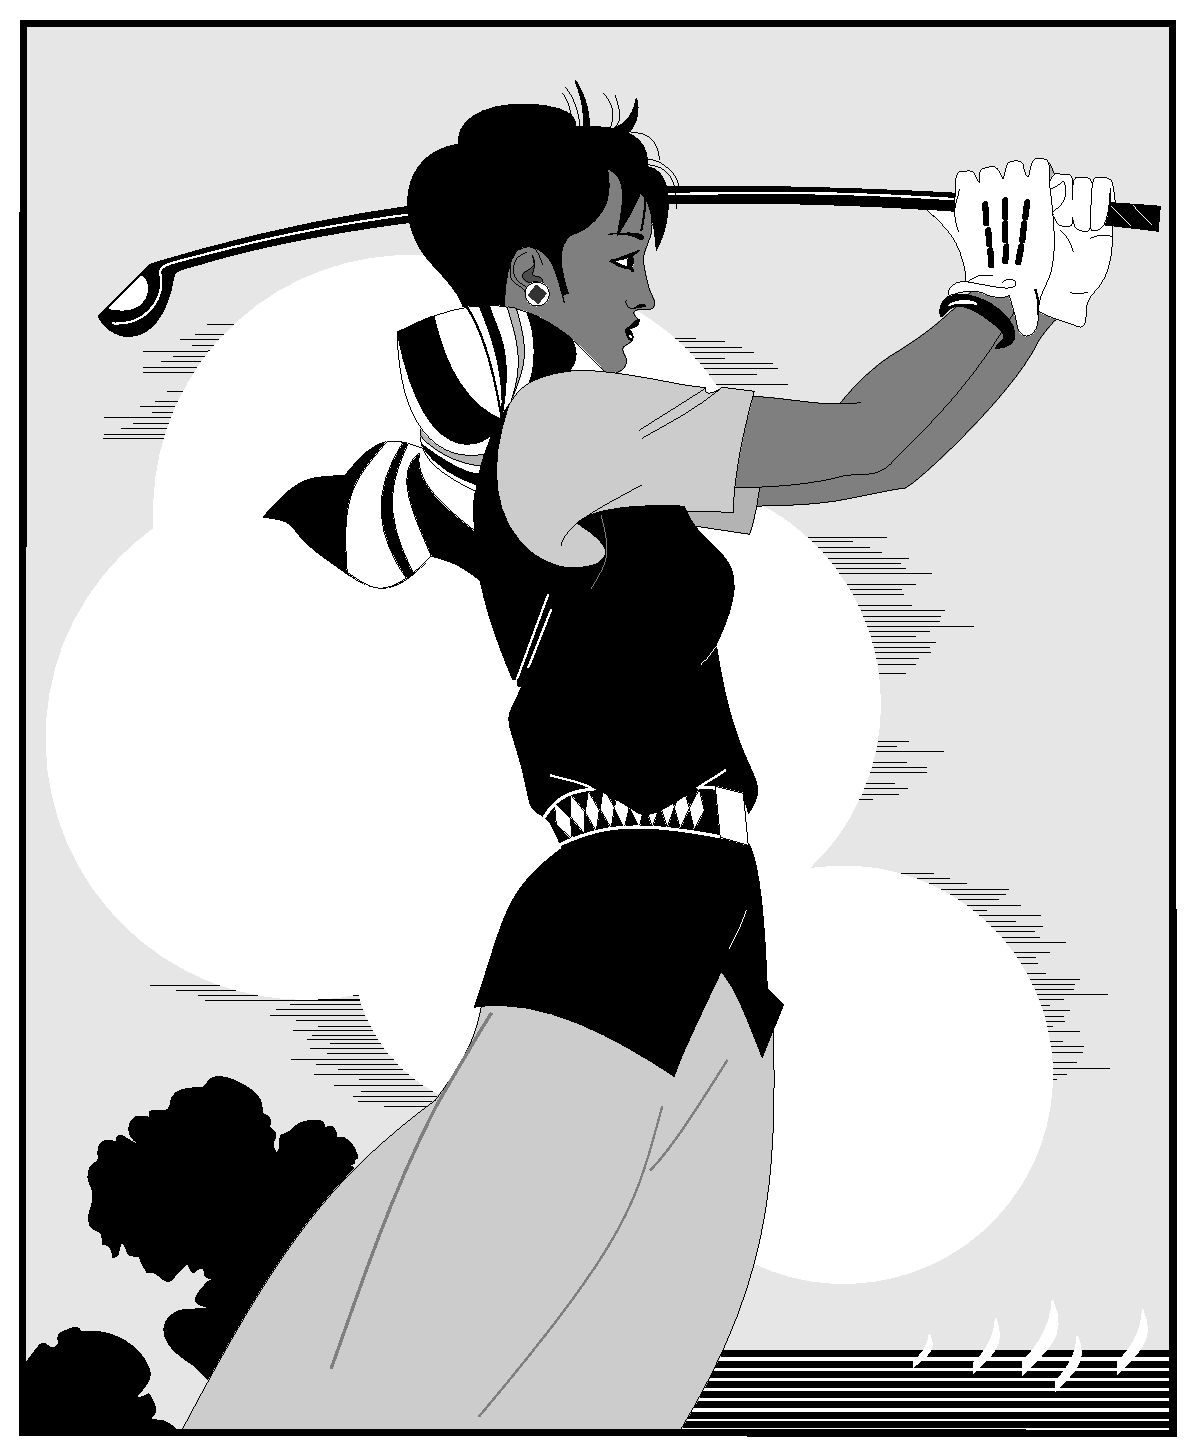
\includegraphics[width = 0.4\textwidth]{golfer}
%\bicaption[golfer5]{}{\xiaosi[0]打高尔夫球的人}{Fig.$\!$}{The person playing golf}\vspace{-1em}
\caption{\xiaosi[0]打高尔夫球的人}
\end{figure}

附录中公式的示例:
\begin{align}
a & = b \times c \\
E & = m c^2
\label{eq}
\end{align}

\chapter{这个星球上最好的免费Linux软件列表}[List of the Best Linux Software in our Planet]
\section{系统}

\href{http://fvwm.org/}{FVWM 自从上世纪诞生以来,此星球最强大的窗口管理器。}
推荐基于FVWM的桌面设计hifvwm:\href{https://github.com/dustincys/hifvwm}{https://github.com/dustincys/hifvwm}。

\subsection{hifvwm的优点}

\begin{enumerate}
	\item 即使打开上百个窗口也不会“蒙圈”。计算机性能越来越强大,窗口任务的管理必须要升级到打怪兽级别。
	\item 自动同步Bing搜索主页的壁纸。每次电脑开机,午夜零点自动更新,用户
		也可以手动更新,从此审美再也不疲劳。
	\item 切换窗口自动聚焦到最上面的窗口。使用键盘快捷键切换窗口时候,减少
		操作过程,自动聚焦到目标窗口。这一特性是虚拟窗口必须的人性化设
		计。
	\item 类似window右下角的功能的最小化窗口来显示桌面的功能此处类似
		win7/win10,实现在一个桌面之内操作多个任务。
	\item 任务栏结合标题栏。采用任务栏和标题栏结合,节省空间。
	\item 同类窗口切换。可以在同类窗口之内类似alt-tab的方式切换。
	\item ……
\end{enumerate}

\section{其他}

\href{https://github.com/goldendict/goldendict}{goldendict 星球最强大的桌面字典。}

\href{https://github.com/yarrick/iodine}{iodine,“HIT-WLAN + 锐捷”时代的福音。}

\href{http://www.aircrack-ng.org/}{aircrack,Wifi“安全性评估”工具。}

\href{https://www.ledger-cli.org/}{ledger,前“金融区块链”时代最好的复式记账系统。}

\href{https://orgmode.org/}{orgmode,最强大的笔记系统,从来没有之一。}

\href{https://www.jianguoyun.com/}{坚果云,国内一款支持WebDav的云盘系统,国内真正的云盘没有之一。}

\href{http://www.mutt.org/}{mutt, ``All mail clients suck. This one just sucks less.''}

\section{vim}
实现中英文每一句一行,以及实现每一句折叠断行的简单正则式,tex源码更加乖乖。
\begin{lstlisting}
vnoremap <leader>fae J:s/[.!?]\zs\s\+/\="\r".matchstr(getline('.'), '^\s*')/g<CR>
vnoremap <leader>fac J:s/[。!?]/\=submatch(0)."\n".matchstr(getline('.'), '^\s*')/g<CR>
vnoremap <leader>fle :!fmt -80 -s<CR>
\end{lstlisting}

% \end{appendix}
% % !Mode:: "TeX:UTF-8" 
\begin{publication}
\noindent\textbf{发表的相关论文}
\begin{publist}
\item	XXX,XXX. Static Oxidation Model of Al-Mg/C Dissipation Thermal Protection Materials[J]. Rare Metal Materials and Engineering, 2010, 39(Suppl. 1): 520-524.(SCI~收录,IDS号为~669JS,IF=0.16)
\item XXX,XXX. 精密超声振动切削单晶铜的计算机仿真研究[J]. 系统仿真学报,2007,19(4):738-741,753.(EI~收录号:20071310514841)
\item XXX,XXX. 局部多孔质气体静压轴向轴承静态特性的数值求解[J]. 摩擦学学报,2007(1):68-72.(EI~收录号:20071510544816)
\item XXX,XXX. 硬脆光学晶体材料超精密切削理论研究综述[J]. 机械工程学报,2003,39(8):15-22.(EI~收录号:2004088028875)
\item XXX,XXX. 基于遗传算法的超精密切削加工表面粗糙度预测模型的参数辨识以及切削参数优化[J]. 机械工程学报,2005,41(11):158-162.(EI~收录号:2006039650087)
\item XXX,XXX. Discrete Sliding Mode Cintrok with Fuzzy Adaptive Reaching Law on 6-PEES Parallel Robot[C]. Intelligent System Design and Applications, Jinan, 2006: 649-652.(EI~收录号:20073210746529)
\end{publist}

\noindent\textbf{(二)申请及已获得的专利(无专利时此项不必列出)}
\begin{publist}
\item XXX,XXX. 一种温热外敷药制备方案:中国,88105607.3[P]. 1989-07-26.
\end{publist}

\noindent\textbf{(三)参与的科研项目及获奖情况}
\begin{publist}
\item	XXX,XXX. XX~气体静压轴承技术研究, XX~省自然科学基金项目.课题编号:XXXX.
\item XXX,XXX. XX~静载下预应力混凝土房屋结构设计统一理论. 黑江省科学技术二等奖, 2007.
\end{publist}
%\vfill
%\hangafter=1\hangindent=2em\noindent
%\setlength{\parindent}{2em}
\end{publication}
    % 所发文章
% \begin{ceindex}
  %如果想要手动加索引,注释掉以下这一样,用wordlist环境
\printsubindex*
\end{ceindex}
    % 索引, 根据自己的情况添加或者不添加,选择自动添加或者手工添加。
\authorization %授权
%\authorization[scan.pdf] %添加扫描页的命令,与上互斥
% !Mode:: "TeX:UTF-8"
\begin{acknowledgements}



\end{acknowledgements}
 %致谢
% % !Mode:: "TeX:UTF-8" 

\begin{resume}
XXXX~年~XX~月~XX~日出生于~XXXX。

XXXX~年~XX~月考入~XX~大学~XX~院(系)XX~专业,XXXX~年~XX~月本科毕业并获得~XX~学学士学位。

XXXX~年~XX~月------XXXX~年~XX~月在~XX~大学~XX~院(系)XX~学科学习并获得~XX~学硕士学位。

XXXX~年~XX~月------XXXX~年~XX~月在~XX~大学~XX~院(系)XX~学科学习并获得~XX~学博士学位。

获奖情况:如获三好学生、优秀团干部、X~奖学金等(不含科研学术获奖)。

工作经历:

\textbf{( 除全日制硕士生以外,其余学生均应增列此项。个人简历一般应包含教育经历和工作经历。)}
\end{resume}
          % 博士学位论文有个人简介
%%%%%%%%%%%%%%%%%%%%%%%%%%%%%%%%%%%%%%%%%%%%%%%%%%%%%%%%%%%%%%%%%%%%%%%%%%%%%%%%
% 博后书序
%%%%%%%%%%%%%%%%%%%%%%%%%%%%%%%%%%%%%%%%%%%%%%%%%%%%%%%%%%%%%%%%%%%%%%%%%%%%%%%%
% \bibliography{reference} % 参考文献
% % !Mode:: "TeX:UTF-8"
\begin{acknowledgements}



\end{acknowledgements}
 %致谢
% % !Mode:: "TeX:UTF-8" 

\begin{doctorpublication}
\noindent\textbf{(一)发表的学术论文}
\begin{publist}
\item	XXX,XXX. Static Oxidation Model of Al-Mg/C Dissipation Thermal Protection Materials[J]. Rare Metal Materials and Engineering, 2010, 39(Suppl. 1): 520-524.(SCI~收录,IDS号为~669JS,IF=0.16)
\item XXX,XXX. 精密超声振动切削单晶铜的计算机仿真研究[J]. 系统仿真学报,2007,19(4):738-741,753.(EI~收录号:20071310514841)
\item XXX,XXX. 局部多孔质气体静压轴向轴承静态特性的数值求解[J]. 摩擦学学报,2007(1):68-72.(EI~收录号:20071510544816)
\item XXX,XXX. 硬脆光学晶体材料超精密切削理论研究综述[J]. 机械工程学报,2003,39(8):15-22.(EI~收录号:2004088028875)
\item XXX,XXX. 基于遗传算法的超精密切削加工表面粗糙度预测模型的参数辨识以及切削参数优化[J]. 机械工程学报,2005,41(11):158-162.(EI~收录号:2006039650087)
\item XXX,XXX. Discrete Sliding Mode Cintrok with Fuzzy Adaptive Reaching Law on 6-PEES Parallel Robot[C]. Intelligent System Design and Applications, Jinan, 2006: 649-652.(EI~收录号:20073210746529)
\end{publist}

\noindent\textbf{(二)申请及已获得的专利(无专利时此项不必列出)}
\begin{publist}
\item XXX,XXX. 一种温热外敷药制备方案:中国,88105607.3[P]. 1989-07-26.
\end{publist}

\noindent\textbf{(三)参与的科研项目及获奖情况}
\begin{publist}
\item	XXX,XXX. XX~气体静压轴承技术研究, XX~省自然科学基金项目.课题编号:XXXX.
\item XXX,XXX. XX~静载下预应力混凝土房屋结构设计统一理论. 黑江省科学技术二等奖, 2007.
\end{publist}
%\vfill
%\hangafter=1\hangindent=2em\noindent
%\setlength{\parindent}{2em}
\end{doctorpublication}
    % 所发文章
% % !Mode:: "TeX:UTF-8" 
\begin{publication}
\noindent\textbf{发表的相关论文}
\begin{publist}
\item	XXX,XXX. Static Oxidation Model of Al-Mg/C Dissipation Thermal Protection Materials[J]. Rare Metal Materials and Engineering, 2010, 39(Suppl. 1): 520-524.(SCI~收录,IDS号为~669JS,IF=0.16)
\item XXX,XXX. 精密超声振动切削单晶铜的计算机仿真研究[J]. 系统仿真学报,2007,19(4):738-741,753.(EI~收录号:20071310514841)
\item XXX,XXX. 局部多孔质气体静压轴向轴承静态特性的数值求解[J]. 摩擦学学报,2007(1):68-72.(EI~收录号:20071510544816)
\item XXX,XXX. 硬脆光学晶体材料超精密切削理论研究综述[J]. 机械工程学报,2003,39(8):15-22.(EI~收录号:2004088028875)
\item XXX,XXX. 基于遗传算法的超精密切削加工表面粗糙度预测模型的参数辨识以及切削参数优化[J]. 机械工程学报,2005,41(11):158-162.(EI~收录号:2006039650087)
\item XXX,XXX. Discrete Sliding Mode Cintrok with Fuzzy Adaptive Reaching Law on 6-PEES Parallel Robot[C]. Intelligent System Design and Applications, Jinan, 2006: 649-652.(EI~收录号:20073210746529)
\end{publist}

\noindent\textbf{(二)申请及已获得的专利(无专利时此项不必列出)}
\begin{publist}
\item XXX,XXX. 一种温热外敷药制备方案:中国,88105607.3[P]. 1989-07-26.
\end{publist}

\noindent\textbf{(三)参与的科研项目及获奖情况}
\begin{publist}
\item	XXX,XXX. XX~气体静压轴承技术研究, XX~省自然科学基金项目.课题编号:XXXX.
\item XXX,XXX. XX~静载下预应力混凝土房屋结构设计统一理论. 黑江省科学技术二等奖, 2007.
\end{publist}
%\vfill
%\hangafter=1\hangindent=2em\noindent
%\setlength{\parindent}{2em}
\end{publication}
    % 所发文章
% % !Mode:: "TeX:UTF-8" 

\begin{resume}
XXXX~年~XX~月~XX~日出生于~XXXX。

XXXX~年~XX~月考入~XX~大学~XX~院(系)XX~专业,XXXX~年~XX~月本科毕业并获得~XX~学学士学位。

XXXX~年~XX~月------XXXX~年~XX~月在~XX~大学~XX~院(系)XX~学科学习并获得~XX~学硕士学位。

XXXX~年~XX~月------XXXX~年~XX~月在~XX~大学~XX~院(系)XX~学科学习并获得~XX~学博士学位。

获奖情况:如获三好学生、优秀团干部、X~奖学金等(不含科研学术获奖)。

工作经历:

\textbf{( 除全日制硕士生以外,其余学生均应增列此项。个人简历一般应包含教育经历和工作经历。)}
\end{resume}
          % 博士学位论文有个人简介
% % !Mode:: "TeX:UTF-8"
\begin{correspondingaddr}
  \heiti\xiaosi
  \noindent 永久通讯地址: \par
  \noindent email: \par
  \noindent 电话: \par
\end{correspondingaddr}
 %通信地址
%%%%%%%%%%%%%%%%%%%%%%%%%%%%%%%%%%%%%%%%%%%%%%%%%%%%%%%%%%%%%%%%%%%%%%%%%%%%%%%%
\end{document}
% Local Variables:
% TeX-engine: xetex
% End:
